%   ,
%    ,   |\ ,__
%    |\   \/   `.
%    \ `-.:.     `\
%     `-.__ `\=====|
%        /=`'/   ^_\
%      .'   /\   .=)
%   .-'  .'|  '-(/_|
% .'  __(  \  .'`
%/_.'`  `.  |`
%    jgs  \ |
%          |/
  
%%%%%%%%%%	TITULO
\date{}
\title{
    \huge{
		\vspace*{-30mm}
	\resizebox{160mm}{28mm}{\color{black}{ABC}}
	\\
	\vspace{8mm}
	\resizebox{160mm}{20mm}{\color{black}\textbf{da Inform\'{a}tica}}
	\\
	\vspace{10mm}
%	\resizebox{260mm}{8mm}{\color{black}{Um Guia do BNCC para Professores Desesperados}}
%	\\
	\vspace{10mm}
	\resizebox{300mm}{14mm}{\color{black}{Sistema para Gerenciamento de Aulas}}
	\\
	\vspace{6mm}
	\resizebox{300mm}{14mm}{\color{black}{em Laborat\'{o}rios de Inform\'{a}tica}}
%\\
%\vspace{2mm}
%\resizebox{160mm}{4mm}{\color{black}{Escola Municipal Professor Paulista - Tabatinga - SP}}
%		\\
%		\vspace{2mm}
%		\resizebox{80mm}{6mm}{\color{black}{Latinoware 2021}}
%		\vspace{5mm}
    }
}

\author {\Huge \\\vspace{2mm}\resizebox{160mm}{10mm}
	{
	\color{black}\Huge Smith{ {\LARGE \&\&} 
%		\Huge D\"{o}rr{ {\LARGE \&\&}
			 {\Huge Aravecchia} {\LARGE \&\&} {\Huge all}}
	}}
%}
%%%%%%%%%%	DOCUMENTCLASS
\documentclass[18pt]{book}
%\usepackage[paperwidth=33cm,paperheight=15cm]{geometry}

%%%%%%%%%%	PAGINA
\newcommand{\papelX}{343mm}
\newcommand{\papelY}{194mm}
\newcommand{\cabecalho}{15mm}
\newcommand{\margem}{20mm}
\newcommand{\rodape}{5mm}
\newcommand{\letra}{5mm}
\newcommand{\distancia}{8mm}
\newcommand{\largura}{\textwidth}
\newcommand{\altura}{\textheight}
\newcommand{\alturaA}{\altura}
\newcommand{\alturaB}{\alturaA-\distancia}
\newcommand{\alturaC}{\alturaB-\distancia}
\newcommand{\alturaD}{\alturaC-\distancia}
\newcommand{\alturaE}{\alturaD-\distancia}
\newcommand{\alturaF}{\alturaE-\distancia}
\newcommand{\alturaG}{\alturaF-\distancia}
\newcommand{\alturaH}{\alturaG-\distancia}
\newcommand{\alturaI}{\alturaH-\distancia}
\newcommand{\alturaJ}{\alturaI-\distancia}
\newcommand{\alturaK}{\alturaJ-\distancia}
\newcommand{\alturaL}{\alturaK-\distancia}
\newcommand{\alturaM}{\alturaL-\distancia}
\newcommand{\alturaN}{\alturaM-\distancia}
\usepackage[portrait, top=\cabecalho,left=\margem,right=\margem,bottom=\rodape, paperwidth=\papelX,paperheight=\papelY]{geometry}

%\setlength{\textwidth}{\largura-\margem}

\setlength{\parindent}{\margem} % indent, o espaçamento inicial horizontal no início um parágrafo
\setlength{\parskip}{3mm plus 10mm} % espaçamento entre um parágrafo e outro

% \setlength{\oddsidemargin}{0mm}
% \setlength{\marginparwidth}{0mm}
\setlength{\topmargin}{-20mm}

%  \setlength{\leftmargin}{-20mm}
\setlength{\headsep}{10mm}
%\setlength{\footskip}{-100mm}
%\setlength{\footnoterule}{50mm}



% Parametros para multicolunas
%\setlength{\premulticols}{1mm}
%\setlength{\postmulticols}{1mm}
%\setlength{\multicolsep}{1mm}
\setlength{\columnsep}{\margem}
\setlength{\textheight}{155mm}
%%%%%%%%%%%%%%%%%%%%%%%%%%%%%%%%%%%%%%%%%%%

%FANCY
\usepackage{fancyhdr}
\pagestyle{fancy}

\lhead{\large \sffamily Sistema de Gerenciamento para Laboratorios de Informatica}

\chead {\large \sffamily \href{https://flisol.info/Brasil}{FLISoL}
\includegraphics[height=7mm]{./IMG/FLISoL-2015-simples.png}}
%\chead{\large \sffamily
%		}
%	
%\lhead{\large \sffamily \blue \textbf{\leftmark}}
\cfoot{\large \sffamily \LaTeX}
\rhead{\large \sffamily Smith, Aravecchia et all}
%\rfoot{\large \sffamily \blue SUA MARCA AQUI}

\rfoot{\Large \sffamily \thepage}
%\rfoot{\normalsize \sffamily \blue \thepage}
\renewcommand{\headrulewidth}{1pt}
\renewcommand{\footrulewidth}{1pt}

%Parametros linguisticos
\pagenumbering{arabic}
\fontencoding{T1}
\usepackage[utf8]{inputenc}
\usepackage[brazil]{babel}

% Define comando BibTeX
\def\BibTeX{{\rm B\kern-.05em{\sc i\kern-.025em b}\kern-.08em
	T\kern-.1667em\lower.7ex\hbox{E}\kern-.125emX}}

% N\~ao imprime numero de se\c c\~ao
%\setcounter{secnumdepth}{0}

\usepackage{multicol}
\usepackage{vwcol}
\usepackage{calc}
\usepackage{ifthen}
\usepackage{graphicx}% Usado para outros tipos de imagens
\usepackage{color}

\usepackage{amsfonts}
\usepackage{amssymb}
\usepackage{float} % Usado para posicionamento de imagens
\usepackage{svg}  % Eis o pacote que queremos.

\usepackage[
colorlinks=true
,linkcolor=blue
,anchorcolor=blue
,urlcolor=blue
]
{hyperref}
\hypersetup{pdftitle={Alexandre Aravecchia}}

\usepackage{calc}
\usepackage{ifthen}
\usepackage{cite}
\usepackage{lipsum}
\usepackage{tikz}
\usepackage{wrapfig}
\usepackage{sidecap}
\usepackage{wallpaper}
\usepackage{lipsum}
\usepackage{xcolor}
\usepackage{tgheros}
\usepackage{amsmath}
\usepackage{amsthm}
\usepackage{textcomp}
\usepackage{enumerate}
\usepackage{pdfpages} % Para inserir páginas de um pdf externo no documento
\usepackage{media9} % Para inserir media no documento


%\usepackage{fontspec} % Para mudar o estilo de todas as fontes (indice, por exemplo).
%\setmainfont{OpenSans} % Altera o estilo de fonte para o corpo do texto.
%\setindexfont{Arial} % Para alterar o estilo de fonte do índice.

\renewcommand{\labelitemi}{$\bullet$}
\renewcommand{\labelitemii}{$\cdot$}
\renewcommand{\labelitemiii}{$\diamond$}
\renewcommand{\labelitemiv}{$\ast$}

\usepackage{enumitem}
\usepackage{courier}
\usepackage{listings}
\usepackage{setspace}
\usepackage{fixme}
\usepackage{csvsimple}

%_______________________________________ LATEXDRAW
\usepackage[usenames,dvipsnames]{pstricks}
\usepackage{epsfig}
\usepackage{pst-grad}
\usepackage{pst-plot}
\usepackage{pgf}
\usepackage{tikz}
\usepackage{pgfplots}
\usepackage{pstricks-add}
\usepackage{tikz-3dplot}
\usepackage{tkz-euclide}
%\usepackage[pdftex]{hyperref}

\usetikzlibrary{arrows, arrows.meta, automata, backgrounds, calendar, chains, matrix, mindmap, patterns, petri, shadows, shapes.geometric, shapes.misc, spy, trees}

\usepackage[european]{circuitikz}

\tikzset{>=latex, %melhor aparência para as setas
    inner sep=0pt,outer sep=0pt %sem separação entre os nós
}

%%%%%% DEFINICAO DE CORES
\definecolor{black}{rgb}{0,0,0}
\definecolor{white}{rgb}{1,1,1}
\definecolor{red}{rgb}{1,0,0}
\definecolor{green}{rgb}{0,1,0.1}
\definecolor{blue}{rgb}{0,0,1}
\definecolor{lightblue}{rgb}{.75,.75,1}
\definecolor{darkblue}{rgb}{0,0,.57}
\definecolor{skyblue}{rgb}{.9,.9,1}
\definecolor{orange}{rgb}{1,.33,0}
\definecolor{gold}{rgb}{1, 0.8, 0.2}
\definecolor{gray}{rgb}{.5,.5,.5}

\pagecolor{white} 
\color{black}
%CHAMADA DE CONFIGURACOES PARA CÓDIGO-FONTE EM ARDUINO
% Template for documenting your Arduino projects
% Author:   Luis Jose Salazar-Serrano
%           totesalaz@gmail.com / luis-jose.salazar@icfo.es
%           http://opensourcelab.salazarserrano.com

%%%%% Template based in the template created by Karol Koziol (mail@karol-koziol.net)

%\linespread{1.3}

\lstdefinestyle{ArduinoStyle}{
	language=C,
	fillcolor=\color{white},
	backgroundcolor=\color{white},
	basicstyle=\small\ttfamily,
	breakatwhitespace=false,
	breaklines=true,
	captionpos=b,
	commentstyle=\color{gray},
	deletekeywords={...},
	escapeinside={\%*}{*)},
	extendedchars=true,
	frame=single,
	keepspaces=true,
	keywordstyle=\bfseries\color{orange},
	morekeywords={*,...},
	numbers=left,
	numbersep=2mm,
	numberstyle=\footnotesize\color{darkgray},
	rulecolor=\color{black},
	rulesepcolor=\color{black},
	showspaces=false,
	showstringspaces=false,
	showtabs=false,
	stepnumber=1,
	stringstyle=\color{orange},
	tabsize=3,
	title=\lstname,
	emphstyle=\bfseries\color{blue},
	framexleftmargin=0mm,
	framextopmargin=1mm
}

%CHAMADA DE CONFIGURACOES PARA CÓDIGO-FONTE EM PYTHON
% Template for documenting your Arduino projects
% Author:   Luis Jose Salazar-Serrano
%           totesalaz@gmail.com / luis-jose.salazar@icfo.es
%           http://opensourcelab.salazarserrano.com

%%%%% Template based in the template created by Karol Koziol (mail@karol-koziol.net)

%\linespread{1.3}

\lstdefinestyle{PythonStyle}{
	language=Python,
	fillcolor=\color{white},
	backgroundcolor=\color{white},
	basicstyle=\small\ttfamily,
	breakatwhitespace=false,
	breaklines=true,
	captionpos=b,
	commentstyle=\color{gray},
	deletekeywords={...},
	escapeinside={\%*}{*)},
	extendedchars=true,
	frame=single,
	keepspaces=true,
	keywordstyle=\bfseries\color{orange},
	morekeywords={*,...},
	numbers=left,
	numbersep=2mm,
	numberstyle=\footnotesize\color{darkgray},
	rulecolor=\color{black},
	rulesepcolor=\color{black},
	showspaces=false,
	showstringspaces=false,
	showtabs=false,
	stepnumber=1,
	stringstyle=\color{orange},
	tabsize=3,
	title=\lstname,
	emphstyle=\bfseries\color{blue},
	framexleftmargin=0mm,
	framextopmargin=1mm
}

%SHELL
% Template for documenting your Arduino projects
% Author:   Luis Jose Salazar-Serrano
%           totesalaz@gmail.com / luis-jose.salazar@icfo.es
%           http://opensourcelab.salazarserrano.com

%%%%% Template based in the template created by Karol Koziol (mail@karol-koziol.net)

%\linespread{1.3}
\lstdefinestyle{C}{
	language=sh,
	fillcolor=\color{white},
	backgroundcolor=\color{white},
	basicstyle=\small\ttfamily,
	breakatwhitespace=false,
	breaklines=true,
	captionpos=b,
	commentstyle=\color{gray},
	deletekeywords={...},
	escapeinside={\%*}{*)},
	extendedchars=true,
	frame=single,
	keepspaces=true,
	keywordstyle=\bfseries\color{orange},
	morekeywords={*,...},
	numbers=left,
	numbersep=2mm,
	numberstyle=\footnotesize\color{darkgray},
	rulecolor=\color{black},
	rulesepcolor=\color{black},
	showspaces=false,
	showstringspaces=false,
	showtabs=false,
	stepnumber=1,
	stringstyle=\color{orange},
	tabsize=3,
	title=\lstname,
	emphstyle=\bfseries\color{blue},
	framexleftmargin=0mm,
	framextopmargin=1mm
}

%\usepackage{npn, ground, vcc, vin, vout, ci, legenda, transistorA, transistorB, transistorC, relay,  ssr, quedadetensao, motorA, motorB, triac, moc, kirchhoff, malha}
%____________________________________________CODIGOS
%lstset{language=Python,
%morecomment={[s][{color{azul}}]{sequencia de 1}{sequencia de caracteres 2}, %diz
%	que todo o texto entre a sequencia de caracteres 1 e a sequencia de caracteres 2 sera um comentario e
%	sera pintada do tipo de cor 1
%	morecomment={[l][{color{tipo de cor 2}}]{sequencia de caracteres}}, % diz que todo o texto a partir da
%	sequencia de caracteres até a o final da linha sera considerado um comentario e sera pintado com tipo de
%	cor 2
%	keywordstyle=[1]color{tipo de cor 3}, %diz que todas as palavras reservadas da linguagem serão
%	pintatadas com o tipo de cor 3.
%
%}
\usepackage{mdframed}%complemento para wallpaper
%'\makeindex
\begin{document}
    \setlength{\footskip}{-10mm}
    \ThisCenterWallPaper{.8}{./IMG/FLISoL-2015-simples.png}
%\ThisULCornerWallPaper{.9}{./IMG/flisol-logo-capa.jpg}
    %\noindent
    \setstretch{1.25} %espacamento entre linhas
    %	\singlespacing % Para um espaçamento simples
    %	\onehalfspacing % Para um espaçamento de 1,5
    %	\doublespacing % Para um espaçamento duplo
    \sffamily
    \pagecolor{white} 
    \color{black}
    \maketitle
%	\CenterWallPaper{1.1}{./IMG3D/MAKER_02.png}		
    %	\CenterWallPaper{1.25}{./IMG/wallpaper.png}
    %			\noindent
    %		\end{itemize}
    %\makebox[235mm][c]{{\includegraphics[height=50mm,width=230mm]{./IMG_2018/FB_IMG_15320316603844789.jpg}}}	\end{itemize}
    %		\makebox[235mm][c]{	\raisebox{-\totalheight}[0mm][0pt]		{\includegraphics[height=\altura-\dXa,width=\largura]{./IMG_2018/FB_IMG_15320316603844789.jpg}}}	
%    \pagebreak
%\pagecolor{black} 
\begin{multicols}{2}

\tableofcontents
\end{multicols}

%    \tableofcontents
%	\CenterWallPaper{1.1}{./IMG3D/MAKER_02.png}	
%    \pagebreak
%\chapter[ Apresentação]{Apresentação}
%\begin{multicols}{2}
%	\begin{multicols}{2}
{\small	Alô meninos e meninas!

Eu sou o Alexandre Aravecchia, designer, desenvolvedor, professor de computação, nerd convito, fui diagnosticado com altas habilidades) ainda na escola primária, eu sou nerd mesmo, raiz!, e, como muitos de vocês, eu sou um sobrevivente.

Eu quero falar uma coisa importante prá vocês, que pode parecer meio óbvia, mas gente \textbf{filha da puta} existe em todo lugar, infelizmente.

Em casa, na família, no trabalho, na escola, na igreja, no círculo de amizades, ao longo de toda sua vida, não é a maioria, mas sempre nós vamos ter que lidar com pessoas que não querem nada além de ver o nosso pescoço pendurado numa forca, ou de preferência numa prisão, onde esta pessoa é o carcereiro e você não consegue sair, por mais que você tente ou se esforce prá fazer tudo bonitinho...

Sempre vai estar faltando alguma coisa práquele tão sonhado prêmio prometido, não é assim?

Você sabe que é.

Acontece que existe uma brecha aí nessa prisão, que o carcereiro esqueceu de fechar, e neste trabalho eu quero mostrar pra vocês uma saída prá essa armadilha.

Curto e grosso:

É a gaiola financeira a primeira coisa que um narcisista vai utilizar contra você, afinal, abra seus olhos:

Ele está sempre em posição de superioridade frente a você, tanto socialmente quanto financeiramente: seja uma mãe ou um pai narcisistas, um marido abusivo ou um chefe aproveitador, ele geralmente é quem manda, e na maior parte do tempo usa contra você uma coisa que ele tem, e você não: dinheiro!

Dentre todas as armadilhas narcisistas que nós podemos cair, acho que a pior de todas é a financeira.

Pense comigo: sem uma colocação profissional, um emprego, um trabalho que coloque dinheiro na tua conta todo mês, como você vai fazer para fugir do cativeiro, e estabelecer o tão sonhado contato zero? Morando na rua?

Acho que não é boa idéia!

Como vai conseguir fazer uma terapia, então? Mesmo que consiga pelo SUS, vocês acham que o narcisista vai deixar você ir assim, sem infernizar sua vida até que você desista?

Então, ao invés de dizer para você trabalhar duro ou lutar como uma fera, para conseguir só ser acorrentado mais e mais, proponho uma coisa: ao invés de trabalhar duro, vamos desta vez usar a cabeça!

Sigam-me os bons!
}
\vfill\null
\pagebreak

\end{multicols}
%\end{multicols}
%section[Apresentação]{Apresentação}
%\begin{multicols}{2}
%	Bora lá?

Somos eu e você, professora, colegas de trabalho, geralmente amigos, e muitas vezes até parentes, então podemos ser sinceros?

O que vou dizer é constrangedor, mas, pergunte a uma criança de 8 anos se ela gosta da escola.

No fundo ela dirá que não, e saberá por quê. Não discuta, ou você irá perder.

Pergunte a ela oq ela não gosta na escola, e você terá um vislumbre do quê é ter 8 anos numa escola publica.

%\end{multicols}
\pagebreak
\color{black}

	\chapter{\sffamily Sobre o Efestus}
	\large \begin{multicols}{2}
Todo Laboratório de Informática de Escola tem um problema: ninguém sabe direito o que fazer ali!

É uma realidade que está mexendo com a vida de todo mundo, não só dos pais e professores.

Isso está colocando em risco o futuro dos nossos jovens (e eu estou falando de futuro prá daqui a \textbf{2 anos}) e compromentendo o funcionamento da própria sociedade como um todo.

Quanta gente não passou aperto durante a pandemia, porque não achava um sobrinho que soubesse fazer um documento online, por exemplo?

E o que dizer dos empregos que esses jovens terão acesso, então?

O problema é que as escolas, muitas vezes, não fazem a menor idéia do que deve ser ensinado sobre Computação para as crianças, principamente nos anos iniciais da alfabetização, que são os mais importantes, porque é na primeira infância que os conceitos básicos de \textbf{lógica} podem ser ensinados corretamente.

\begin{itemize}
\item Joãozinho, pegue uma \{camiseta verde \textbf{e} vermelha\}.

\item Joãozinho, pegue uma \{camiseta verde \textbf{ou} vermelha\}.

	\item Joãozinho, pegue \{1 camiseta verde\} \textbf{e} \{1 camiseta vermelha\}.
	
		\item Joãozinho, pegue \{1 camiseta verde\} \textbf{ou} \{1 camiseta vermelha\}.
\end{itemize}

Notou a diferença, professor(a)?

Pensa comigo:

\begin{itemize}
	\item Você que ralou e estudou 4 anos de pedagogia, letras, história, biologia, sabe mesmo o fazer, pra sua turma de 4\textordmasculine\space ano:

		\begin{itemize}
			\normalsize
		\item entrar no google
	\item pesquisar sobre um determinado assunto
	\item baixar 4 ou 5 imagens pro HD
	\item colocar tudo isso num editor de texto
	\item escrever um texto
	\item diagramar o documento
	\item colocar tipos e tamanhos de fontes, margens, espaçamentos, etc.
	\item salvar o documento do aluno num lugar onde você possa encontrar depois
	\item imprimir 20 documentos
	\end{itemize}
\end{itemize}

Você consegue mesmo ensinar tudo isso, em \textbf{50 minutos}?

E você, \textbf{coordenador}, sabe dizer detalhadamente, qual o conteúdo de Computação que precisa ser ensinado, do 1\textordmasculine\space ao 9\textordmasculine\space ano, e quais são as ferramentas digitais que o Laboratório de Informática precisa disponibilizar pros alunos, aula por aula?

As escolas:

\begin{itemize}
	\item não conhecem as ferramentas que têm à disposição
	\item não sabem que essas ferramentas são todas gratuitas
	\item não têm um plano de aulas pro professor seguir
	\item não têm uma estratégia de ensino de computação
	\item não sabem lidar com a questão da cyber-segurança
	\item mal têm um planejamento (quando têm), que se adequa à realidade dos alunos e ao equipamento da escola
 \item e principalmente: não têm uma \textbf{ferramenta}, um software que organize toda essa informação, e gerencie as atividades no computador de cada aluno.
\end{itemize}

Além disso, nossos professores não tiveram o devido preparo prá lidar com a tecnologia computacional, na escala que nós enfrentamos hoje.

Não tem como um professor, que ralou e estudou 4 anos de licenciatura em História, por exemplo, saber o mínimo de HTML (assim como eu também não sei nada sobre Vigotsky).

E não basta a escola ter um plano de aulas de Computação.

Hoje nós já estamos melhor, temos o \textbf{BNCC de Tecnologia}, que é um plano metodológico, mas \textbf{ainda não é um plano de aulas}.

É uma \textbf{orientação metodológica}: na prática, serve para que a escola possa criar seu plano de aulas, adaptado à sua própria realidade, conforme a legislação disponível \href{http://portal.mec.gov.br/index.php?option=com_docman&view=download&alias=241671-rceb001-22&category_slug=outubro-2022-pdf&Itemid=30192}{neste link}.

Além desse plano de aulas, para que ele funcione, a escola precisa de um \textbf{software prá gerenciar tudo isso}, no computador que está na mão de cada aluno!

Por isso, o professor \textbf{Ole Smith}, da UFG, me propôs este desafio: criar um banco de dados que a escola pudesse utilizar, para montar seu próprio plano de aulas pro Laboratório de Informática, que o próprio aluno pudesse acessar, do seu computador.

E que ainda o professor não precisasse se desesperar, prá fazer sua aula, num ambiente que ele não está acostumado, onde ele não foi devidamente treinado nem orientado prá trabalhar, que é o Laboratórios de Informática.

Assim surgiu o \textbf{ABC da Informática}, um plano de aulas de Computação, que eu venho desenvolvendo com crianças do Ensino Fundamental, e adaptando conforme as diretrizes do BNCC a cada faixa etária, há mais de 10 anos.

Não é um plano de aulas perfeito, nem está completo ainda, mas é um plano de aulas que funcionou prá mim e pros meus alunos, e ficarei feliz se ele servir de ponto de partida para outros professores e instrutores de Informática.

Mas não é apenas é um documento, é também um banco de dados, que qualquer Escola pode copiar, modificar, e adaptar livremente, à sua própria realidade e ao seu projeto pedagógico.

Basta o coordenador ou cada professor preencher sua lista de atividades em formato texto TXT, o instrutor ou técnico de TI converter para \LaTeX, e o script gera tanto um arquivo PDF, que o professor leva no celular, como uma pagina HTML, que vai para o servidor Apache da escola.

Assim, disponibilizando todas as atividades na rede local da escola, como página inicial de todos os computadores dos alunos, o professor entra com os alunos no Laboratório, e a atividade já está lá, numa lista préviamente preparada para cada aula individual, do 1\textordmasculine ao N\textordmasculine ano, aula por aula, o ano todo.

O \textbf{Sistema Efestus} serve prá gerenciar tudo isso, e fazer com que cada atividade chegue pra cada aluno, automaticamente, e na hora certa.

O professor têm à mão uma biblioteca inteira de textos, imagens links para diversas atividades, aplicativos, programas, tudo o que ele precisar para servir de apoio à sua aula.

O projeto é todo disponibilizado em \textbf{Software Livre}, com licença não comercial, e você pode baixá-lo neste link \href{https://github.com/aravecchia/HEFESTUS/blob/main/HEFESTUS.pdf}{\textbf{\Large aqui}}.

Lá você vai encontrar um PDF com toda a descrição do projeto, e um plano de aulas para Computação, do 1\textordmasculine\space ao 5\textordmasculine\space ano fundamental, que é a faixa etária que eu trabalho.

Mas você pode adaptá-lo a qualquer faixa etária, e também para qualquer disciplina, como Letras ou História, por exemplo, se sua escola tiver um técnico que conheça \href{https://www.latex-project.org}{\LaTeX}, HTML, Apache e Linux.

Também você vai encontrar diversos links para atividades, o código-fonte de todo o projeto, textos da Wikipedia, imagens, diagramas, códigos de programação, tudo o que você mesmo escolher, prá você ensinar pros seus alunos, esquemas de experimentos com robótica educacional, e mais um monte de materiais que serão úteis, prá você ensinar computação pros seus alunos da maneira \textbf{certa}: a maneira do \textbf{Software Livre}, ensinando as bases do pensamento computacional.

Fique a vontade prá baixar o projeto, copiar, distribuir e modificar.

Mostre para o seu cordenador, para o diretor da sua escola e, se puder, compartilhe com outros professores, porque você já vai estar contribuindo muito com o ensino de Tecnologia na sua escola!

	\begin{center}
	
	
\includegraphics[width=.4\linewidth]{./IMG-GIT/tux.png}

\end{center}
\vfill
\end{multicols}

\pagebreak
\section{\sffamily LEIA-ME.tex}


\LARGE Manual de Instrucões.

		\begin{multicols}{2}
	
	\normalsize	De forma geral, o sistema é muito simples: uma página HTML, gerada em \LaTeX, e disponibilizado  numa página do servidor Apache local.
	
	Então configuramos todos os computadores dos alunos, para que abram esta página automaticamente, através do navegador, logo na inicialização do seu Desktop Linux favorito.
	
	É uma tarefa que pode ser realizada por qualquer técnico ou profissional de TI, que tenha acesso à senha root do sistema, alguns conhecimentos em redes, HTML, Apache, e saiba usar minimamente o terminal, habilidades mínimas para qualquer instrutor de Informática.
	
	Quanto à linguagem \LaTeX, você não terá dificuldades em aprender o básico, rápidamente.
	
	Desta forma, basta o Instrutor ligar os computadores e, e em poucos minutos, os alunos terão na tela um índice de todas as aulas e atividades, de todos  os bimestres, de todos os anos letivos, e o professor terá não somente um guia de aulas, mas todo o Universo que quiser criar em hipertexto, desde aulas expositivas, imagens, videos, jogos, simuladores espaciais, tudo o que é necessario para transformar aquilo que seria só mais uma aula chata, numa grande viagem de exploração pelo universo digital!
	
	E fazemos isso de forma simples, automática, rápida, eficiente, pedagogicamente correta, livre de pirataria e ainda sem custos adicionais para a Escola, pois todo o sistema é desenvolvido em Software Livre.
	
	As atividades escritas por mim, que constam neste documento, foram testadas ao longo de 10 anos, em sala de aula, em turmas de 15 a 20 alunos, de 6 a 15 anos, mas é cruxial lembrar que o BNCC permite que cada Escola, professor ou instrutor encontre sua própria metodologia, e desenvolva seu próprio roteiro de aulas, de acordo com as necessidades de cada turma ou Escola.
	
	Justamente por este motivo, este documento é liberado sob licença Creative Commons, em formato de código aberto: para que as aulas sejam editáveis por qualquer escola, professor ou instrutor que queira fazê-lo.
	
	Sinta-se a vontade para copiar, alterar e distribuir cópias, observando a licença \textbf{Creative Commons Não Comercial}.
	
	Um ano letivo tem aproximadamente 8 meses, com 4 aulas cada um. Ou seja, 32 aulas anuais, para cada ano de ensino. Se temos uma escola de 5 anos, resulta num total de 160 aulas, independente do número de alunos.
	
	Então são 160 arquivos em formato texto editaveis, um para cada aula.
	
	No \LaTeX, estes arquivos podem ser tanto um texto, como podem carregar imagens, ou ate uma biblioteca inteira de imagens, assim como links para diversas atividades, como aplicativos, programas, páginas web ou arquivos salvos na máquina local, ou mesmo num servidor externo.
	
	Utilizando \LaTeX, criamos um arquivo HTML, que pode ser lido em qualquer celular que esteja conectado à rede local da escola, propiciando ainda mobilidade ao professor, ja que também pode leva-lo para casa, no formato PDF.
	
	Este mesmo PDF e transformado em formato HTML, através de um script simples.
	
	%Para isso, primeiro e necessario instalar o pacote poppler-utils:
	%
	%\begin{lstlisting}
	%	apt install poppler-utils
	%\end{lstlisting}
	
Se você é iniciante em Linux, a primeira coisa que precisa aprender a fazer é \textbf{usar o terminal}.

Não se assuste, com o tempo e um pouco de prática, você pega o jeito.

Vamos lá: mantenha pressionada a tecla Alt no teclado e aperte F2. Vai aparecer uma janela parecida com essa: 

\begin{center}
	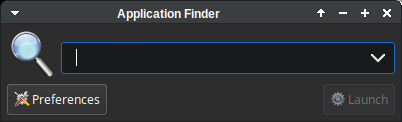
\includegraphics[width=\linewidth]{./IMG-GIT/Screenshot_20231222_142820.png}
\end{center}

Ali, digite \textbf{xterm} (tudo em letras minúsculas) e aperte \textbf{Enter}.

Vai aparecer uma janela, mais ou menos assim:


\begin{center}
	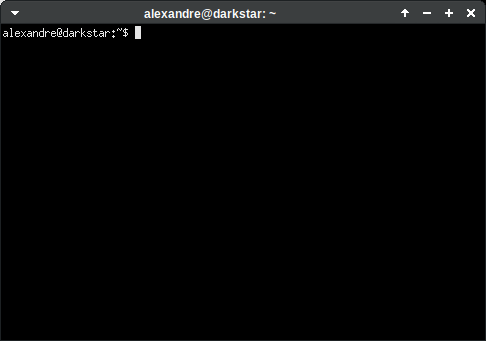
\includegraphics[width=\linewidth]{./IMG-GIT/Screenshot_20231222_143805.png}
\end{center}

	Bem vindo ao maravilhoso mundo de \textbf{/bin/bash}, que é como nós chamamos o terminal, o \textbf{ambiente hacker} propriamente dito.
	
	Sabe \textbf{aquela tela preta que você vê nos filmes}? É isso!
	
	Prá nós entendermos, de um jeito simples, veja que está escrito \textbf{alexandre@darkstar:$\sim\$$}.
	
	Se você tem um \textbf{e-mail}, vai ver que ele sempre é um \textbf{nome de usuário + um servidor}, ou seja, é você, em algum um computador, em algum lugar do mundo.
	
	O meu, por exemplo:
	
	\begin{center}
		{\large aravecchia@gmail.com}
	\end{center}

\textbf{aravecchia} é meu \textbf{nome de usuário} no computador (servidor) \textbf{gmail.com}.

No meu computador, meu nome de usuário é \textbf{alexandre}, e o nome do computador é \textbf{darkstar}, ou seja, \textbf{alexandre@darkstar}.

No computador da escola, meu nome de usuário é \textbf{professor}, e o nome do computador central é \textbf{servidor}, então meu usuário naquele computador é \textbf{professor@servidor}.

O importante é que temos sempre \textbf{usuario@computador}, é simples.

Agora vamos nos tornar um usuário especial: \textbf{root}, também chamado de superusuário, ou simplesmente \textbf{DEUS} (porque ele pode fazer tudo o que quiser)\footnote{\begin{multicols}{2}{Acostume-se às piadas sarcásticas ca computação, professor(a). Elas podem ser chatas, e algumas vezes muito inconvenientes, mas também são muito úteis didaticamente, para que os alunos lembrem-se de conceitos básicos importantes da computação. Responta rápido: Qual a diferença entre \textit{software} e \textit{hardware}?}
		content...
\end{multicols}}.

Para isso, vamos digitar desta forma no terminal:

	\lstinputlisting[style=C, label=lst:CCode]
{./SCRIPTS-GIT/passwd.sh}

Perceba que, quando você digita a senha, no Linux, nenhum caractere aparece no terminal. Não se preocupe, isto é pra garantir a segurança da tua senha.

Prefira uma senha fácil de lembrar, combinando letras e números, e não perca \textbf{nunca}! Ou você estará em sérios apuros!

Agora digite:

	\lstinputlisting[style=C, label=lst:CCode]
{./SCRIPTS-GIT/su.sh}

Pronto!

Agora você é \textbf{root}, o superusuário, senhor do seu próprio destino, guardião e comandante do terminal.

Você não é mais um simples usuário!

\begin{center}
	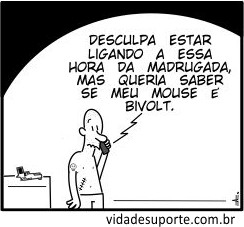
\includegraphics[width=.4\linewidth]{./IMG-GIT/Suporte_643.jpg}
\end{center}	

	Agora olhe novamente para a última linha do seu terminal, e você verá algo parecido com isto:
	
	\begin{center}
		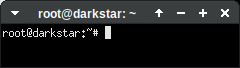
\includegraphics[width=.6\linewidth]{./IMG-GIT/Screenshot_20231222_155332.png}
	\end{center}	

Você é o usuário \textbf{root}, supremo comandante do computador \textbf{darkstar}.

Agora vamos instalar algumas coisinhas, e brincar com as permissões de acesso ao sistema.


	\begin{lstlisting}
		pdf2htmlEX PROJETO.pdf index.html
		
		pdftohtml [options] [pdf source file] [html output file]
		
		pdftohtml -v PROJETO.pdf index.html
	\end{lstlisting}
	
	
	O HTML resultante vai para a página Apache do servidor local, e todos os outros computadores são direcionados a ela, na inicialização.
	
	\begin{lstlisting}
sudo passwd root\\
(digite 2x a nova senha de root)
		
su -\\
Password:
		
apt update
		
apt -f install openssh-server openssh-client apache tomcat9 arduino frozen-bubble debian-junior gcompriz...
		
chown -vR professor /var/lib/tomcat9/webapps/ROOT/index.html
		
chown -vR professor /var/www/html/index.html
	\end{lstlisting}
	
	\begin{lstlisting}
pdf2htmlEX PROJETO.pdf index.html
		
cp -v index.html /var/lib/tomcat9/webapps/ROOT/index.html
		
cp -v index.html /var/www/html/index.html
	\end{lstlisting}
	
\end{multicols}



%SHELL
% Template for documenting your Arduino projects
% Author:   Luis Jose Salazar-Serrano
%           totesalaz@gmail.com / luis-jose.salazar@icfo.es
%           http://opensourcelab.salazarserrano.com

%%%%% Template based in the template created by Karol Koziol (mail@karol-koziol.net)

%\linespread{1.3}
\lstdefinestyle{C}{
	language=sh,
	fillcolor=\color{white},
	backgroundcolor=\color{white},
	basicstyle=\small\ttfamily,
	breakatwhitespace=false,
	breaklines=true,
	captionpos=b,
	commentstyle=\color{gray},
	deletekeywords={...},
	escapeinside={\%*}{*)},
	extendedchars=true,
	frame=single,
	keepspaces=true,
	keywordstyle=\bfseries\color{orange},
	morekeywords={*,...},
	numbers=left,
	numbersep=2mm,
	numberstyle=\footnotesize\color{darkgray},
	rulecolor=\color{black},
	rulesepcolor=\color{black},
	showspaces=false,
	showstringspaces=false,
	showtabs=false,
	stepnumber=1,
	stringstyle=\color{orange},
	tabsize=3,
	title=\lstname,
	emphstyle=\bfseries\color{blue},
	framexleftmargin=0mm,
	framextopmargin=1mm
}


\begin{multicols}{2}
	\normalsize
	
	Supondo que você sabe instalar um sistema operacional GNU de Kernel Linux, sugerimos utilizar uma distribuição baseada em Debian, Ubuntu, ou, de preferência um a distro especializada em educação, como Linux Educacional, Zorin.
	
	Ubuntu Studio revelou-se uma distribuição uma distribuição muito leve, estável e customizável.
	
	Distribuicões que utilizam Desktops mais leves, como Xubuntu ou Lubuntu, são indicadas para computadores mais antigos, de forma a aproveitar melhor os recursos de memória e processamento.
	
	Escolhida a distribuição, a primeira coisa a fazer é, óbviamente, instalar o sistema operacional, criando um usuário \textit{professor}, com privilégios de \textit{sudoer} ou \textit{admin}.
	
	Feito isto, instalado o sistema \textit{default}, vamos trocar a senha de \textit{root}, para facilitar nosso trabalho.
	
	No computador central do Laboratório (servidor, escolha aquele que tiver mais poder de processamento e memória, pois é nele que você vai passar os próximos anos da sua vida):
	
	Acesse sua área de trabalho, com a senha de usuário administrador (usuário "professor", criada durante a instalação), e abra o terminal, utilizando o atalho Alt+F2.
	
	Na caixa que aparecer na tela, digite \textit{xterm} ou \textbf{terminal}, e aperte Enter.
	
	A próxima janela é o terminal, não precisa ter medo dele! Na verdade, com o tempo, você vai passar a gostar muito dele!
	
	Digite no terminal, nesta ordem:



	Repare que, ao digitar a senha, nenhum caractere é escrito no terminal. Isto serve para proteger a nova senha de olhares maliciosos.
	
	Pronto. Agora você é ROOT, tem poderes supremos sobre a máquina.
	
	Por enquanto, vamos nos divertir com os novos super-poderes. Digite:
	
	
	Aperte Enter, digite sua senha de \textit{root} e confirme, apertando ENTER.
	
	Ótimo, agora você tem controle total do servidor!
	
\textbf{Bem vindo ao mundo Linux, Padawan!}
	
Lembre-se, daqui por diante: \textbf{com grandes poderes, grandes responsabilidades você terá}!
	
	O próximo passo é instalar todos os aplicativos didáticos que os alunos utilizarão, bem como todas as ferramentas administrativas e protocolos de rede. Este script deve ajudá-lo:
	
	\lstinputlisting[style=C, label=lst:CCode]
{./SCRIPTS-GIT/install.sh}
	
	Reinicie o servidor, afim de que todos os novos serviços e protocolos instalados sejam carregados corretamente.
	
	Repita esta operação em \textbf{todos os computadores, de todos os alunos}.
	
\textbf{\Large Segue o link para o Github do projeto:}

(Baixe o arquivo ZIP e descompacte na sua pasta Home)
\end{multicols}

\begin{center}
	\Huge	\href{https://github.com/aravecchia/HEFESTUS}{https://github.com/aravecchia/HEFESTUS}
\end{center}

\vfill\null

\pagebreak

\begin{multicols}{2}
\Large Conhecimentos necessarios:
%
%txt $\rightarrow$ tex $\rightarrow$ html $\rightarrow$ apache $\rightarrow$ crontab $\rightarrow$ firefox $\rightarrow$ localhost $\rightarrow$ ssh


	\large
	\begin{itemize}
		\item Shell
		\item \LaTeX
		\item HTML
		\item Apache
		
		\vfill \null
		\columnbreak
		
		\Large Conhecimentos desejaveis:
		
		\item Python
		\item Eletrônica
		\item Arduino
	\end{itemize}
	
\end{multicols}
	\vfill \null
	\pagebreak

\begin{center}
	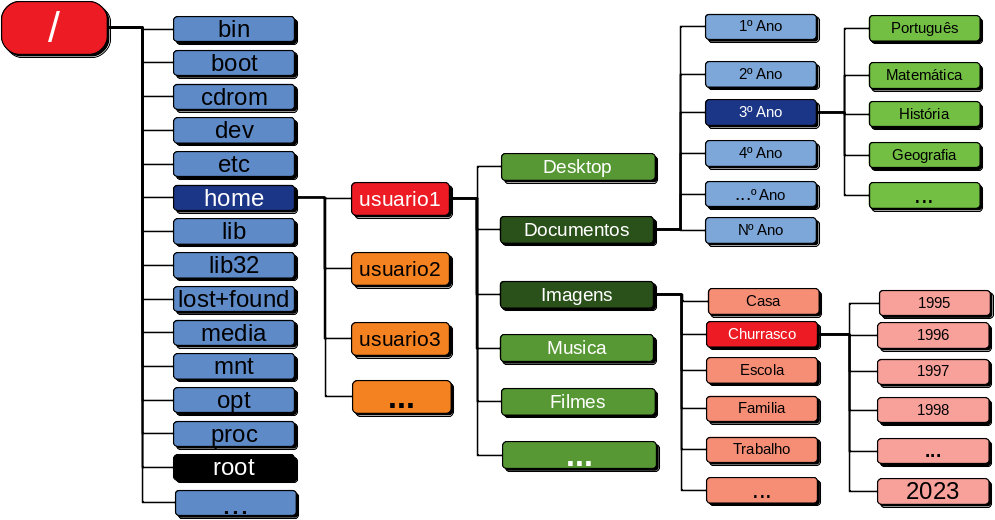
\includegraphics[height=\textheight]{./IMG-GIT/SVG/DIAGRAMAS.png}
\end{center}
\pagebreak

\begin{center}
	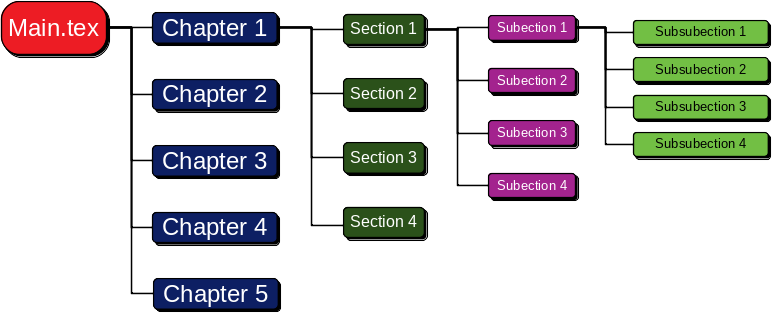
\includegraphics[width=\linewidth]{./IMG-GIT/SVG/DIAGRAMAS2.png}
\end{center}
\pagebreak


\begin{center}
	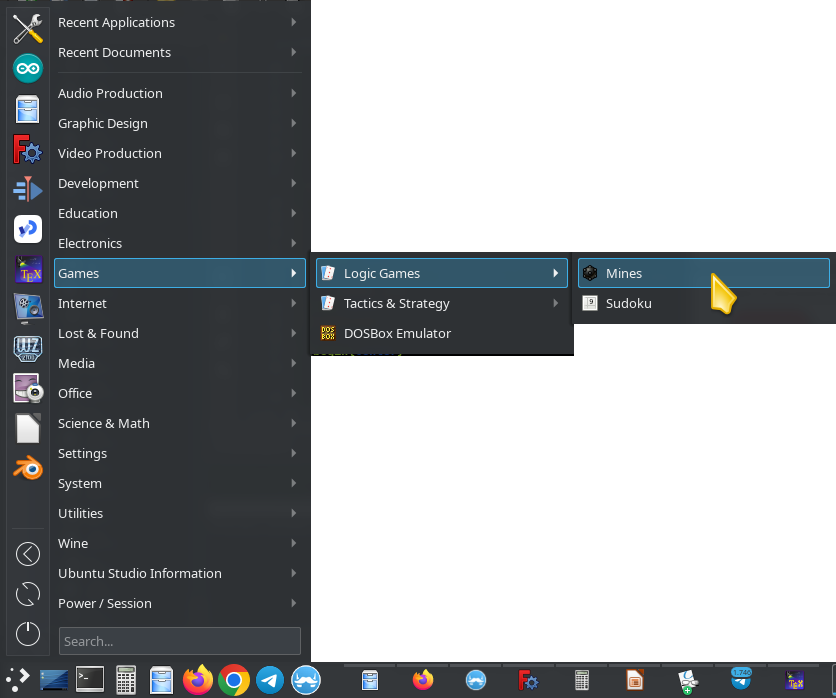
\includegraphics[height=\textheight]{./IMG-GIT/menu.png}
\end{center}
\pagebreak

{\Huge \LaTeX}
\begin{center}
	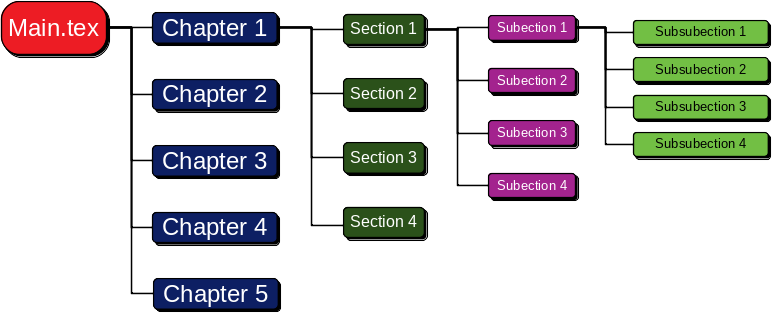
\includegraphics[width=\linewidth]{./IMG-GIT/SVG/DIAGRAMAS2.png}
\end{center}
\pagebreak

\begin{center}
	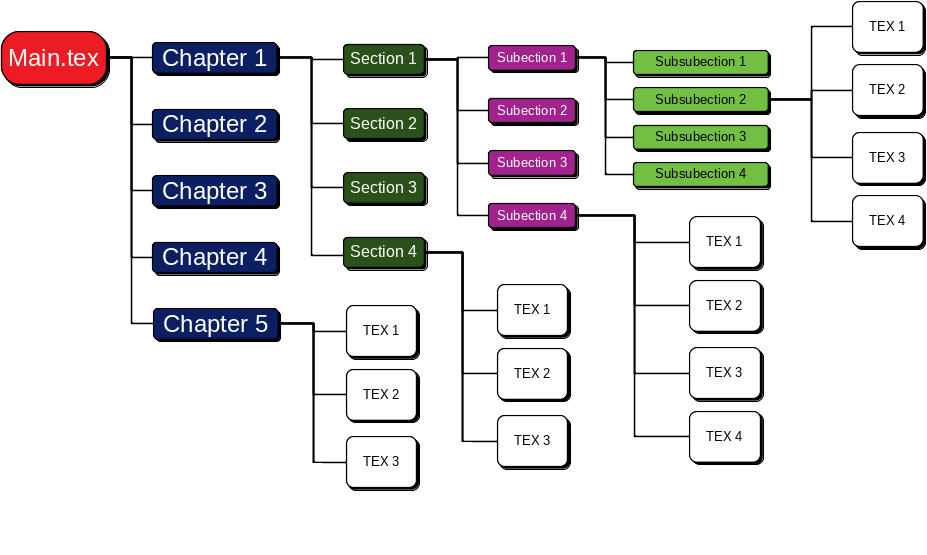
\includegraphics[height=\textheight]{./IMG-GIT/SVG/DIAGRAMAS3.png}
\end{center}
\pagebreak

\begin{center}
	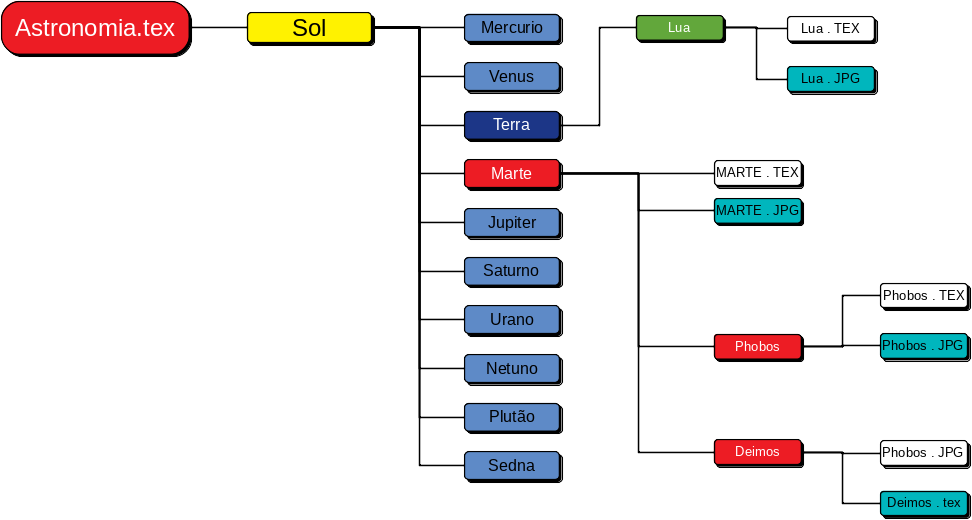
\includegraphics[height=\textheight]{./IMG-GIT/SVG/DIAGRAMAS4.png}
\end{center}
\pagebreak

\begin{center}
	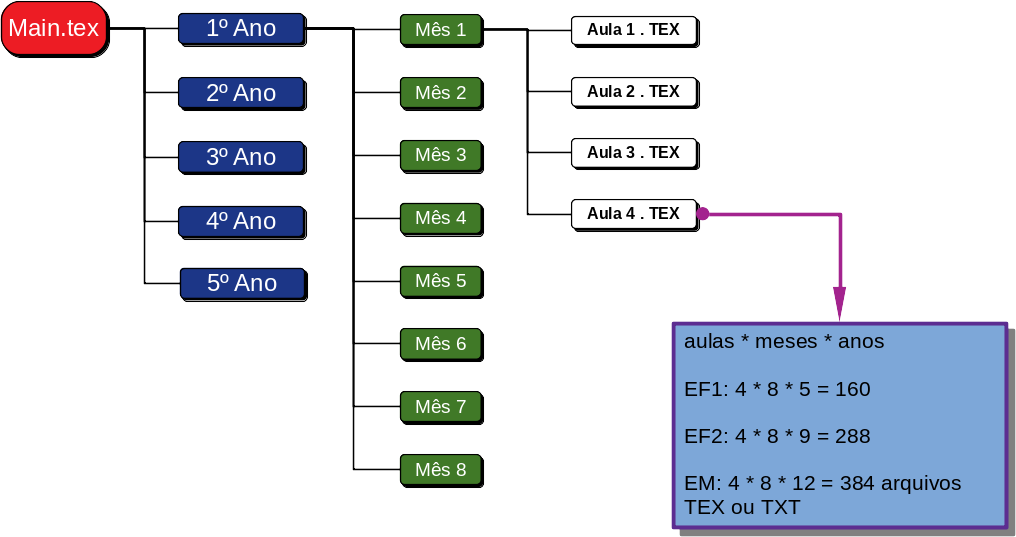
\includegraphics[height=\textheight]{./IMG-GIT/SVG/DIAGRAMAS5.png}
\end{center}
\pagebreak

\begin{center}
	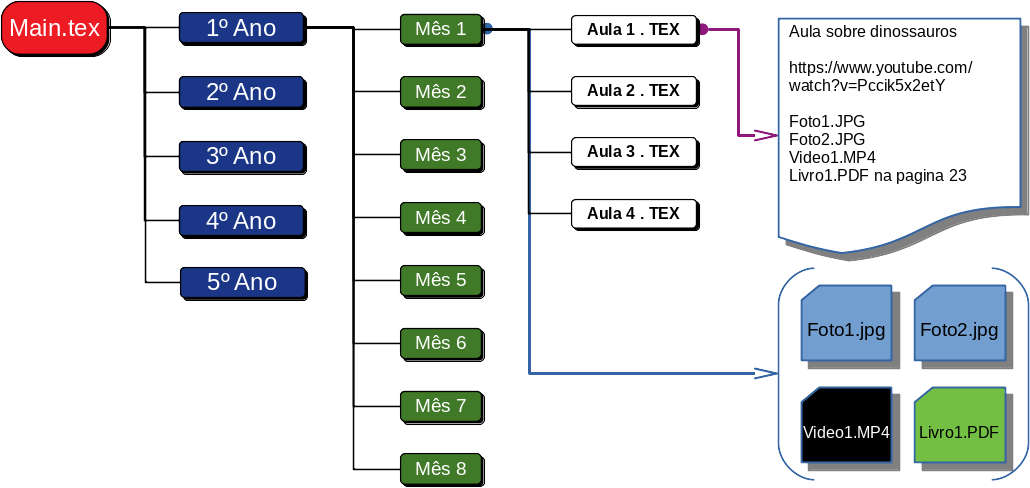
\includegraphics[width=\linewidth]{./IMG-GIT/SVG/DIAGRAMAS6.png}
\end{center}
\pagebreak


\begin{center}
	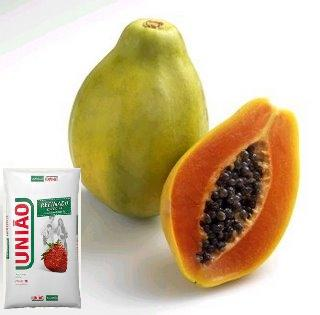
\includegraphics[height=\textheight]{./IMG-GIT/mamao.jpg}
\end{center}
\pagebreak

\begin{multicols}{2}
	\LARGE	 \textbf{Coisas que não vao acontecer}:
	
	\vspace*{10mm}
	\Large \textbf{Querido instrutor}:
	\large
	\begin{itemize}
		\item Quero um video sobre \nobreak dinossauros.
		
		\item Qual video, 'fessora?
		
		\item Não sei, coloca qualquer um.
		
		\item \textbf{Depois}: Mas não foi isso que eu pedi!
		
		\item Esse video não tem nada a ver com o projeto pedagógico da escola...
		
	\end{itemize}
	\vfill\null
	\columnbreak
	
	\begin{center}
		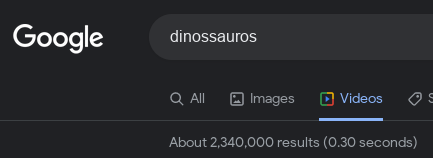
\includegraphics[width=\linewidth]{./IMG-GIT/dinossauros.png}
	\end{center}
	
	\textbf{Link}:
	\large
	\begin{itemize}
		\item https://www.youtube.com/watch?v=Pccik5x2etY
		\item \verb|\href{URL}{Dinossauros}|
		\item \href{https://www.youtube.com/watch?v=Pccik5x2etY}{Dinossauros}
	\end{itemize}
	
	
	\vfill\null
	\columnbreak
	
	\begin{center}5
		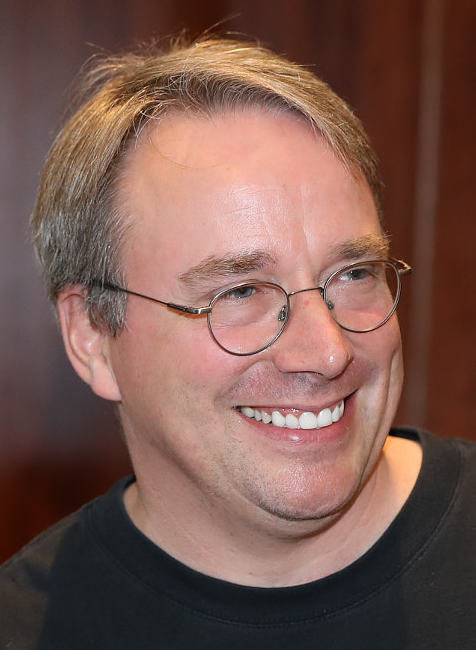
\includegraphics[height=.8\textheight]{./IMG-GIT/linus.jpeg}
	\end{center}
	
	\columnbreak
	\Large \textbf{AULAS que não vao acontecer}:
	
	\vspace*{5mm}
	
	\Large S. Alexandre, preciso fazer uma \nobreak atividade no Word:
	
	\large
	\begin{itemize}
		\item Baixar uma imagem do Google.
		\item Importar para um documento.
		\item Escrever um texto no Frontwork.
		\item Salvar o documento.
		\item Imprimir.
		\item Criancas de 9 anos, iniciantes.
		\item \textbf{50 minutos}.
	\end{itemize}
	
	%Com um tema, d ́a-se maior sentido a inser ̧c ̃ao de se ̧c ̃oes, pois al ́em de serem destacadas nos slides, podemos
	%transitar de uma para outra conforme queiramos.
	%2.5 Organiza ̧c ̃ao das informa ̧c ̃oes na lˆamina
	%A partir dos temas, podemos come ̧car a trabalhar com outras ferramentas importantes para a organiza ̧c ̃ao da
	%apresenta ̧c ̃ao.
	%2.5.1 Blocos
	%Um recurso interessante de organiza ̧c ̃ao de informa ̧c ̃oes  ́e a cria ̧c ̃ao de blocos dentro dos frames, o qual permite
	%criar um conjunto de informa ̧c ̃oes separadas com um t ́ıtulo. Isto  ́e feito atrav ́es dos seguintes comandos:
	%\frame{
		%	\begin{block}{T ́ıtulo do bloco}
			%		...
			%	\end{block}
		%	Estes blocos ser ̃ao separados em caixas que, na lˆamina, aparecer ̃ao em destaque.
		%	Exemplo 8 Utilizando o preˆambulo que foi constru ́ıdo no Exemplo 7, vamos inserir dois blocos em um frame.
		%	\begin{document}
			%		\frame{
				%			\frametitle{Exemplo 8}
				%			\begin{block}{Exemplo de bloco 1}
					%				Aqui escrevemos o texto do bloco 1.
					%			\end{block}
				%			\begin{block}{Exemplo de bloco 2}
					%				Aqui escrevemos o texto do bloco 2.
					%			\end{block}
				%		}

			\vfill \null
			\columnbreak
			
			\begin{center}
%				\vspace{20mm}
				\resizebox{\linewidth}{.3\textheight}{\color{black}\textbf{404}}
				\\
				\vspace*{5mm}
				{\Huge Aula não encontrada}
			\end{center}

	\vfill\null
	\columnbreak
	
	\begin{itemize}
				\item Pagina offline
				\item Sistema desatualizado ou incompatível
				\item Eu peguei no site do MEC, procura lá...
				\item É um video que tem o dinossauro subindo a montanha pra beber água numa cachoeira...
				\item Tá aqui no livro...
				\item Quando chegar o dia a gente vê...
				\item \textbf{Me ajuda, eu tô desesperado(a)!}
				\item \textbf{Eu não sei o que é pra fazer...}
			\end{itemize}
			
		\end{multicols}
	
			
	\vfill
	\pagebreak
		
		\vspace*{30mm}
	\begin{center}
			{\Huge \color{blue} Se a atividade não for programada, não tem atividade!}
	\end{center}
		
		\vfill\null
		\pagebreak
		
		\begin{center}
			
\includegraphics[height=.7\textheight]{./IMG-GIT/anjo.jpg}
			
			\resizebox{\linewidth}{20mm}{\color{magenta}\textbf{Não tem aula de Informática!}}
			
		\end{center}
		\vfill
		\pagebreak
		
		\ThisCenterWallPaper{1.2}{./IMG-GIT/enchente.jpg}
		\begin{center}
			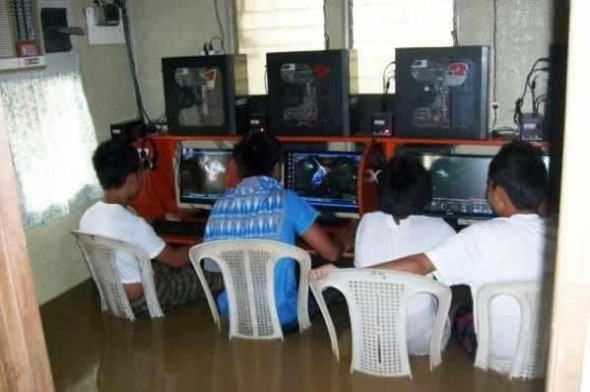
\includegraphics[height=.9\textheight]{./IMG-GIT/enchente.jpg}
		\end{center}
		
		\vfill
		\pagebreak
		
		\begin{frame}
			
			\centering % Para centralizarmos o vídeo
			\includemedia[
			label=nome-qualquer, % ! Importante para linkar o vídeo ao botao (ver abaixo)
			width=0.8\linewidth, height=0.5\linewidth, % Dimensões
			addresource=./MP4-GIT/VOGON.mp4, % ESTE É O SEU ARQUIVO DE VÍDEO (mesmo dir.)
			transparent, % Opcões para que o player tenha transparência
			activate=pageopen, % Se você deseja que o vídeo esteja "carregado" ao abrir a página
			flashvars={
				source=./MP4-GIT/VOGON.mp4
				&loop=false % Se você quer que o vídeo repita automaticamente 
				&scaleMode=letterbox % Manter proporcões (dimensionais) do vídeo
			}
			]{}{./MP4-GIT/VOGON.mp4}
			\vspace{1cm} % Espacamento entre vídeo e botao
			
			% Agora, você cria o botao para dar play/pause. Neste caso, o botao e apenas a letra "pi".
			
			%	\mediabutton[
			%	mediacommand=nome_qualquer:playPause,
			%	overface=\color{black}{{\strut $\pi$}},
			%	downface=\color{gray}{{\strut $\pi$}}
			%	]{{\strut $\pi$}}
			
			
		\end{frame}
		
		\vfill
		\pagebreak
		
		
		\begin{multicols}{3}	
			\begin{center}
				
\includegraphics[height=.5\textheight]{./IMG-GIT/fada.jpeg}
			\end{center}
			\begin{flushright}
				
\includegraphics[height=15mm]{./IMG-GIT/whatsapp.png}
			\end{flushright}
			
			\vfill	
			\columnbreak
			
			\begin{center}
				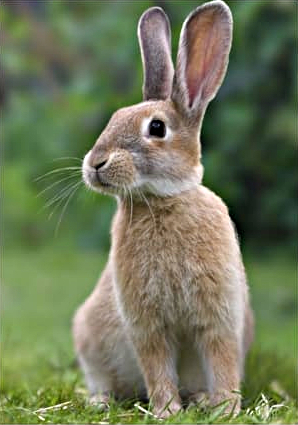
\includegraphics[height=.5\textheight]{./IMG-GIT/coelhinho.jpeg}
			\end{center}
			\begin{flushright}
				
\includegraphics[height=15mm]{./IMG-GIT/whatsapp.png}
			\end{flushright}
			
			\vfill	
			\columnbreak
			
			\begin{center}
				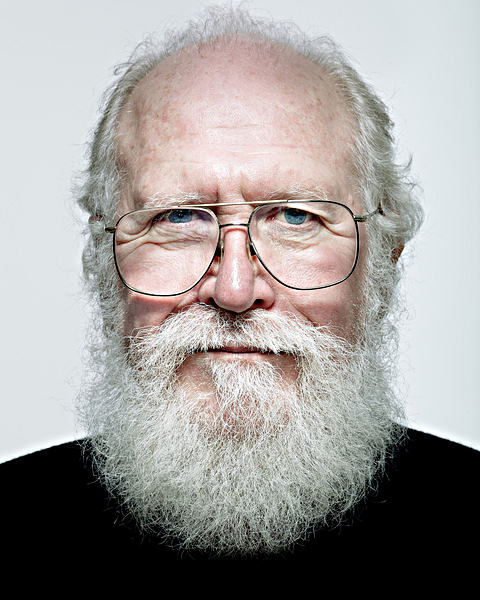
\includegraphics[height=.5\textheight]{./IMG-GIT/maddog.jpg}
			\end{center}
			\begin{flushright}
				
\includegraphics[height=15mm]{./IMG-GIT/whatsapp.png}
			\end{flushright}
		\end{multicols}	
		
		\vfill
		\pagebreak
		
		\begin{center}
			
\includegraphics[height=.7\textheight]{./IMG-GIT/anjo.jpg}
			
			\resizebox{.8\linewidth}{25mm}{\color{magenta}\textbf{É fácil!}}
			
		\end{center}
		\vfill
		\pagebreak
		
		\begin{center}
			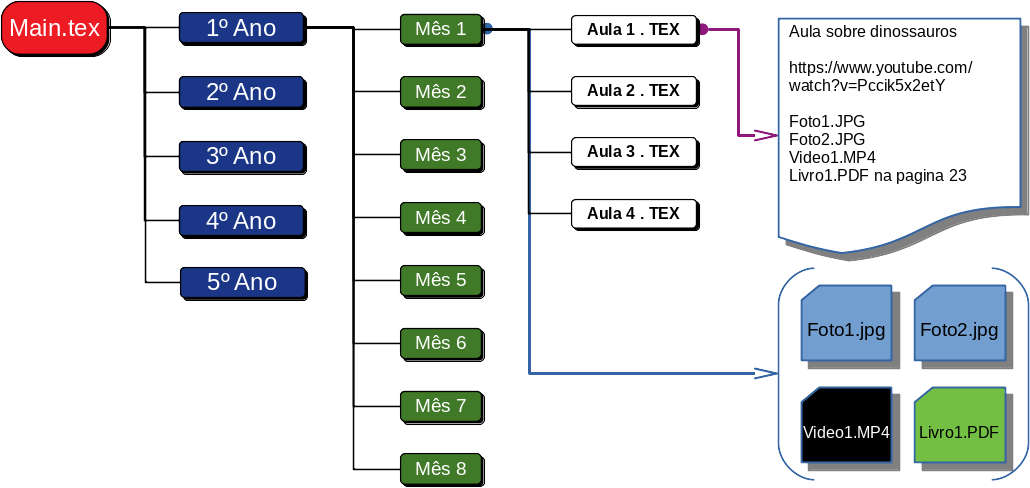
\includegraphics[width=\linewidth]{./IMG-GIT/SVG/DIAGRAMAS6.png}
		\end{center}
		\pagebreak
		
		\begin{center}
			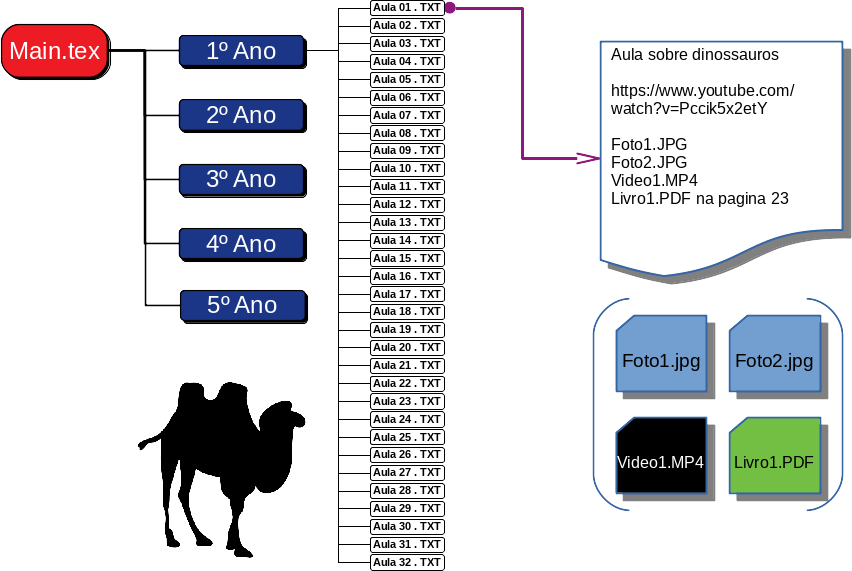
\includegraphics[height=\textheight]{./IMG-GIT/SVG/DIAGRAMAS7.png}
		\end{center}
		\pagebreak
		
		\begin{center}
			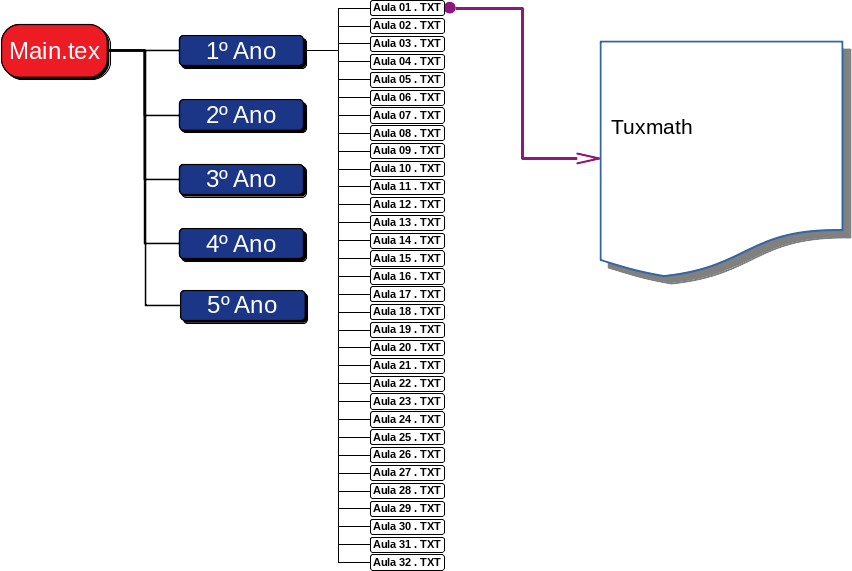
\includegraphics[height=\textheight]{./IMG-GIT/SVG/DIAGRAMAS8.png}
		\end{center}
		\pagebreak
		
		\begin{center}
			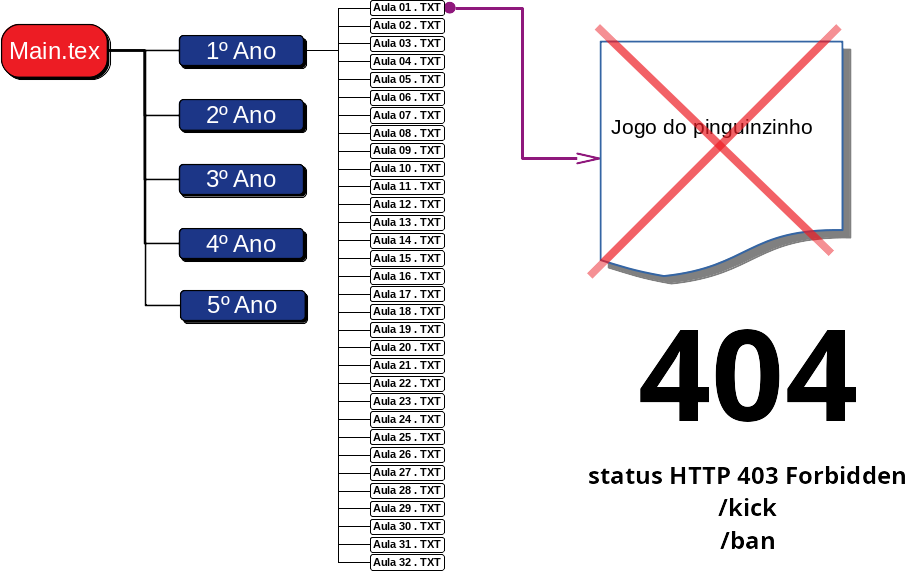
\includegraphics[height=.\textheight]{./IMG-GIT/SVG/DIAGRAMAS9.png}
		\end{center}
		
		\null
		\pagebreak


\section{\sffamily Sobre a versão 1.0}
\begin{multicols}{2}
	{\normalsize
		Esta versão do Código Viking acrescenta diversas melhorias.
		
		O preâmbulo está bem mais enxuto e organizado, foram eliminados todos os pacotes redundantes ou conflitantes. Também foram organizados conforme categorias e receberam os devidos comentários, explicando a função básica de cada um, afim de facilitar estudos mais aprofundados.
		
		Também troquei todas as fontes por OpenSans (sugestão do Cadunico), melhorei as proporções entre tamanho de fonte, margens e distâncias em geral, em relação ao tamanho da página, que agora é proporcional ao tamanho das telas de notebook e celular.
		
		Os tamanhos e proporções escolhidos também geram menos problemas, se caso for necessário ajustar a pagina às pressas, para uso em uma tela mais antiga, como é comum em palestras em lugares onde você nunca esteve (e por isso não conhece o equipamento). Ou ainda imprimir os documentos em papel A4, por exemplo, e precisar diminuir o tamanho das fontes, para economizar papel.
		
		Este mesmo preâmbulo será utilizado em 3 documentos que considero importantes: 
		
		1. \textbf{Be-A-Ba da Informática}: um guia para aulas de informática.
		
		As melhorias desta versão permitem o uso de iteração, provas lógicas, conversão de números binários para decimais e importação de códigos em C, Shell e Python.
		
		Desta forma, o Be-a-Bá da  Informática poderá fazer o que se propôs, quando publicado originalmente na Revista Espirito Livre: ensinar código binário e o básico de Ciência da Computação para crianças, através de recursos gráficos simples.
		
		2.\textbf{ EFESTUS}: Sistema de Gerenciamento para Laboratórios de Informática.
		
		Feito para atender especialmente escolas públicas, um sistema que funciona como um livro didático interativo, em formato hipertexto, onde a escola pode automatizar o cronograma de atividades em seus Laboratórios de Informática, conforme seu próprio planejamento, de acordo com os parâmetros do BNCC, bastando que tenha um Instrutor de Informática ou técnico familiarizado com LaTeX, HTML, GNU-Linux e Apache (fácil).
		
		Conforme a escola adiciona ou altera o arquivo relacionado a um dia letivo qualquer (por exemplo, AULA-5-23.TEX, referente a 23a. aula do 5o. ano), o sistema Efestus gera automaticamente um HTML no servidor local Apache da escola.
		
		Quando o aluno liga o computador, é direcionado para esta página, onde pode buscar a atividade numa lista, seja ela um texto, imagem, apresentação de slides, video, aplicativo na máquina local ou qualquer página web, a escolha do professor.
		
		3. \textbf{Qualquer documento} para apresentação de projetos, palestras ou aulas em geral.
		
		Divirtam-se, nobres guerreiros!}
\end{multicols}

\null
\pagebreak


\section{\sffamily Contribuições}
\begin{multicols}{2}
{
\large
O \textbf{Sistema Efestus} foi escrito com base no \textbf{Código Viking}, projeto iniciado em 2015, durante o \textbf{Fórum \nobreak Goiano de Software Livre} (FGSL), por iniciativa minha, a partir do trabalho e das idéias do prof. \textbf{Dr. Ole Peter Smith}, da Universidade Federal de Goiania, com a generosa contribuição da Comunidade Latino Americana de Software Livre, e a finalidade de potencializar o \textbf{ABC da Informática}, outro projeto relacionado ao ensino de Computação, cujas bases haviam sido lançadas na \textbf{Revista Espirito Livre}, alguns anos antes.

Naquele encontro - \textbf{FGSL 2015} - manifestei meu descontentamento em relação à linguagem HTML, quando o professor Ole Smith me apresentou o \textbf{\LaTeX}.

Pude então ver de perto os códigos-fonte que a Universidade Federal de Goiania utiliza para gerenciar não só o processo educacional, como também o controle de frequência e as notas dos alunos.

Tudo de forma simples, rápida, fácil e automática.

Falamos exaustivamente também das dificuldades de se implantar o ensino de Computação em todas as escolas públicas do Brasil.

Então observei que, se um sistema em \LaTeX\space pode gerenciar os cursos de uma Universidade do tamanho da UFG, por quê não um simples Laboratório de Informática de uma escola municipal? 

Afinal, seria um sistema muito mais simples, com a vantagem de poder ser aplicado em larga escala: se resolvêssemos para o Laboratório de uma escola, resolveríamos para todos os Laboratórios de todas as escolas Brasil.

Por quê ninguem havia pensado nisso antes? - perguntei.

Resposta: o professor Ole havia pensado, há muito tempo.

Porém, dadas as dificuldades de se fazer Educação neste país, simplesmente ninguém havia ainda conseguido escrever este código.

Em 2018, tive a honra de reencontrar o professor Ole Smith na \textbf{Latinoware} - Fórum Latino Americano de Software Livre e Tecnologias Abertas, às vesperas da aprovação do BNCC de Tecnologia.

Na ocasião, pude apresentar ao \textbf{prof. Dr. Julio Cesar Neves}, o pai do Ensino de Computação no Brasil, o notável desenvolvimento dos alunos da Escola Professor Paulista, utilizando o \textbf{ABC da Informática}, gerenciado pelo \textbf{Sistema Efestus}.

Discutia-se, na época, se os Laboratórios de Informática deveriam ensinar Ciência da Computação, ou ser apenas mais um apêndice no processo de alfabetização.

Os alunos do Professor Paulista provaram, na ocasião, que crianças não apenas são capazes de dominar os computadores muito melhor e mais rápido que os adultos, mas também podem aprender programação em linguagem Shell e Python, além de fazer isso brincando!

Exercitando o \textbf{pensamento educacional} da maneira correta e nas fases corretas do desenvolvimento infantil, não só foram capazes de se alfabetizar alguns meses mais cedo, como também dominar a matemática muito melhor e mais rápido, do que se fossem estimuladas apenas pelos métodos tradicionais.

Melhor ainda: o aprendizado se tornou uma atividade divertida para as crianças, uma brincadeira, tanto quanto a Educação Física!

Diversas outras pessoas e comunidades contribuiram para que tais resultados fossem obtidos, e destaco aqui os professores Tiago Sodré, Jefer Dörr, Karina Menezes, Daniel Basconcelos, Débora Garofalo, Ana Diniz e Zoraide Sgarbi.

Também merecem destaque as contribuições do C3SL-UFPR, Hacker Club Cascavel, Raul Hacker Club, Portal Embarcados, Portal Labirito, Laboratório de Garagem, comunidade Debian-BR, comunidade \LaTeX-BR, Instituto Newton Braga e toda a Communidade Latinoware.}
\end{multicols}

\vfill
\pagebreak

\section{\sffamily Licença}
\begin{center}
	
\includegraphics[width=\linewidth]{./IMG-GIT/Cc_by-nc_icon.svg.png}


\href{https://creativecommons.org}{\Huge Creative Commons Atribuída e Não-Comercial}

\end{center}
\vfill\null
\pagebreak

\section{\sffamily O Código Viking}
\large
\begin{multicols}{2}
	A ideia do Código Viking é ser a base \LaTeX \space de trabalho para qualquer professor, tanto para organizar seu plano de trabalho, como para preparar suas aulas, escrever seus livros e artigos, ou desenvolver suas palestras, de forma rápida, fácil, com uma diagramação perfeita, digna de um bom professor.

Assim, surgiu também a idéia do \textbf{Sistema Efestus}, que incorpora scripts Shell e Python ao sistema operacional, para disponibilizar o plano de aulas numa rede local e organizar o trabalho nos Laboratórios de Informática, em escolas públicas de todo o Brasil.

Ja o \textbf{ABC da Informática} é um plano de aulas pessoal, meu, que incorporei a este documento, como exemplo do funcionamento do Código Viking, e para testar o Sistema Hefestus em sala de aula.

Você pode utilizá-lo a vontade, para fins não comerciais, como ponto de partida para criar seu próprio plano de aulas ou gerenciar o Laboratório da sua escola.

Sinta-se à vontade para enviar dúvidas ou sugestões para aravecchia@gmail.com.

Copie, modifique (mantendo os direitos autorais), divulgue e compartilhe!

\vfill\null
\columnbreak

\subsection[Preâmbulo]{Preâmbulo}

\lstinputlisting[basicstyle=\ttfamily, style=LaTeXStyle, label=lst:LaTeXCode]{./HEFESTUS.tex}

\vfill
\columnbreak

\subsection[Capítulo]{Capítulo}

\lstinputlisting[style=LaTeXStyle, label=lst:LaTeXCode]{./CAPITULOS-HEFESTUS.tex}

\subsection[Pacote Listings para códigos-fonte]{Pacote Listings para códigos-fonte}

\begin{verbatim}
	\lstinputlisting[style=LaTeXStyle, label=lst:ArduinoCode]
	{./TeX-git/ARDUINO-CODE.tex}

\lstinputlisting[style=LaTeXStyle, label=lst:ShellCode]
{./TeX-git/SHELL-CODE.tex}

\lstinputlisting[style=LaTeXStyle, label=lst:LaTeXCode]
{./TeX-git/LATEX-CODE.tex}

\lstinputlisting[style=LaTeXStyle, label=lst:LaTeXCode]
{./TeX-git/PYTHON-CODE.tex}
\end{verbatim}

\subsection[Exemplos de códigos-fonte em pacote Listings]{Exemplos de códigos-fonte em pacote Listings}


\lstinputlisting[style=ArduinoStyle, label=lst:ArduinoCode]
{./TeX-git/Arduino-CODE.tex}

\lstinputlisting[style=C, label=lst:CCode]
{./TeX-git/C-CODE.tex}

\lstinputlisting[style=LaTeXStyle, label=lst:LaTeXCode]
{./TeX-git/LaTeX-CODE.tex}

\lstinputlisting[style=PythonStyle, label=lst:PythonCode]
{./TeX-git/Python-CODE.tex}

\end{multicols}

\vfill\null
\pagebreak



		\chapter{\sffamily Querido(a) professor(a):}

%		\begin{multicols}{2}
{\small	Alô meninos e meninas!

Eu sou o Alexandre Aravecchia, designer, desenvolvedor, professor de computação, nerd convito, fui diagnosticado com altas habilidades) ainda na escola primária, eu sou nerd mesmo, raiz!, e, como muitos de vocês, eu sou um sobrevivente.

Eu quero falar uma coisa importante prá vocês, que pode parecer meio óbvia, mas gente \textbf{filha da puta} existe em todo lugar, infelizmente.

Em casa, na família, no trabalho, na escola, na igreja, no círculo de amizades, ao longo de toda sua vida, não é a maioria, mas sempre nós vamos ter que lidar com pessoas que não querem nada além de ver o nosso pescoço pendurado numa forca, ou de preferência numa prisão, onde esta pessoa é o carcereiro e você não consegue sair, por mais que você tente ou se esforce prá fazer tudo bonitinho...

Sempre vai estar faltando alguma coisa práquele tão sonhado prêmio prometido, não é assim?

Você sabe que é.

Acontece que existe uma brecha aí nessa prisão, que o carcereiro esqueceu de fechar, e neste trabalho eu quero mostrar pra vocês uma saída prá essa armadilha.

Curto e grosso:

É a gaiola financeira a primeira coisa que um narcisista vai utilizar contra você, afinal, abra seus olhos:

Ele está sempre em posição de superioridade frente a você, tanto socialmente quanto financeiramente: seja uma mãe ou um pai narcisistas, um marido abusivo ou um chefe aproveitador, ele geralmente é quem manda, e na maior parte do tempo usa contra você uma coisa que ele tem, e você não: dinheiro!

Dentre todas as armadilhas narcisistas que nós podemos cair, acho que a pior de todas é a financeira.

Pense comigo: sem uma colocação profissional, um emprego, um trabalho que coloque dinheiro na tua conta todo mês, como você vai fazer para fugir do cativeiro, e estabelecer o tão sonhado contato zero? Morando na rua?

Acho que não é boa idéia!

Como vai conseguir fazer uma terapia, então? Mesmo que consiga pelo SUS, vocês acham que o narcisista vai deixar você ir assim, sem infernizar sua vida até que você desista?

Então, ao invés de dizer para você trabalhar duro ou lutar como uma fera, para conseguir só ser acorrentado mais e mais, proponho uma coisa: ao invés de trabalhar duro, vamos desta vez usar a cabeça!

Sigam-me os bons!
}
\vfill\null
\pagebreak

\end{multicols}

\ThisCenterWallPaper{1}{./IMG/marvin.jpg}

\begin{multicols}{2}
\huge Não entre em pânico!

\vfill\null
\pagebreak

\normalsize

Eu sei dos tempos sombrios e caminhos tortuosos você trilhou, até chegar aqui, professor/professor(a)!

Sei também das tempestades que se apresentam no horizonte, e conheço o mal que aflige seu coração:

A chegada do novo \textbf{BNCC de Tecnologia}, que impõe o \textbf{ENSINO de COMPUTAÇÃO} em todas as escolas, a partir de 2023. (Leia \href{http://portal.mec.gov.br/index.php?option=com_docman&view=download&alias=241671-rceb001-22&category_slug=outubro-2022-pdf&Itemid=30192}{\textbf{aqui}}).

\vfill\null
\columnbreak

Mas não entre em pânico: você não está sozinho(a)!

Este material veio para te ajudar a enfrentar os desafios que a tecnologia colocou em seu caminho!

\textbf{Eu sei, eu sei, eu sei...}

Ja sei de tudo o que você vai dizer, professor(a).

Decor e salteado!

Sei que você vai reclamar da vida, do Universo e tudo mais, todo dia, na cabeça do instrutor de Informática... 

Mas o medo leva à raiva, e a raiva leva ao caminho sombrio da Força.

Você só vai encontrar dor e sofrimento, se continuar por aí, professor(a).

Computadores só funcionam de um jeito, pelo menos neste Universo:  por meio de códigos binários, \textbf{zero e um}, ponto.

\textbf{Simples assim}!

%Por isso, aquele "\textbf{jeitinho}", que as pessoas estão muitas vezes acostumadas a encontrar, em muitas situacões adversas, no dia-a-dia, este jeitinho simplesmente \textbf{não existe}, quando falamos de computadores.

O computador não é como um carro, que pode andar com o pneu quase cheio.

No computador, o "pneu"\space está \textbf{cheio} ou \textbf{não}!

Não existe meio termo, ou margem para negociação, nem jeitinho, muito menos norma burocrática maliciosa que possa mudar isso.

A menos que você possa alterar as leis da Física.

%Computadores só entendem código binario, e ponto: não têm desejos, emocões, nem qualquer tipo de empatia ou desprezo pela nossa mísera existência mortal.
%
%Seres fascinantes!
%
%Pois eles têm um lado sublime: são máquinas! Se não têm desejos ou sentimentos, portanto, são confiaveis e precisos, de uma forma que nenhum ser humano jamais sera!

%Não foi à tôa, que Sarah Connor confiou a segurança de seu filho John ao esterminador do futuro.

%E estão ficando cada vez mais espertos, muito espertos e incrivelmente rápidos!
%
%Talvez, justamente por isso, despertem tanto fascínio e horror em nós, humanos, demasiadamente humanos.

Computadores são máquinas, cujo funcionamento deve ser sempre muito preciso, e devidamente programado, \textbf{previamente}.

Eles respondem \textbf{somente} da forma que foram \textbf{programados} para responder.

Não espere um bolo de laranja ali, se você o alimentou com bananas!

E alguém ainda tem que programar a receita \textbf{antes} de ligar o "forno", \textbf{e por escrito}, ou também não tem "bolo" \space nenhum.

\textbf{A brincadeira acaba aí, com uma turma de crianças frustradas, e um(a) professor(a) desesperado(a), reclamando do Instrutor de Informática} que, acredite ou não, e o único que ainda está ali tentando te ajudar.

Mas nesta hora, professor(a), você só pode \textbf{reclamar com o Universo}, porque é assim que ele funciona.

Não mate o mensageiro: é assim que os elétrons se movem pelo tecido espaco-tempo, pelo menos neste Universo, \textbf{a menos que você possa alterar as leis da Física}.

Lhamento!

Funciona assim: \textbf{se} a professor(a) quer uma aula, esta aula tem necessariamente que ser programada por \textbf{alguém}, de um jeito ou de outro, e pasmem: \textbf{por escrito}!

Não é programar "qualquer joguinho": você tem que programar \textbf{UM} determinado jogo (ou UMA determinada atividade didatica ESPECÍFICA), todo dia, para cada fase de aprendizado, cada aula, numa sequencia precisa.

Fazendo as contas, são \textbf{384 aulas}, se considerarmos do 1\textordmasculine\space ano Fundamental ao 3\textordmasculine\space ano do ensino Médio.

\textbf{Boa sorte, coordenador(a)!}

\textbf{Divirta-se}!

Mas lembre-se de que, se é muito trabalho escrever o resumo de 384 aulas, mesmo que seja \textbf{copiando da caderneta}, digitar 2 milhões de linhas de código é trabalho \textbf{impossível}, por mais qualificado, nerd, gênio ou superdotado que seja o instrutor de Informática!

Mas calma, professor(a): \textbf{é para isso que os computadores servem}!
 
Desde que você os trate com carinho e o devido respeito, eles são capazes de fazer coisas incríveis, que farão os olhinhos dos seus alunos brilharem!
 
 Garanto: sua aula nunca mais será a mesma!

Pois bem, \textbf{é disTRo que trata este material}:

\textbf{Um Sistema de Gerenciamento para Laboratórios de Informática, que pode ser adaptado a qualquer disciplina, com qualquer Projeto Pedagógico, de qualquer Escola, nos termos do BNCC, e que sirva para criar, editar, gerenciar e distribuir todas as atividades didaticas, pela própria rede local da escola, de maneira facil, rápida, livre, gratuita, segura e \underline{automática}.
}

E tem que ser automático, seu Alexandre?

Tem, professor(a): não existe outro meio, mas é justamente aí que a mágica acontece!

É aí que uma turminha, mesmo aquela considerada das mais fracas, consegue se alfabetizar alguns meses mais cedo que a média, e dispara as notas no IDEB, contando a tabuada "nos dedinhos".

É o que fazem as grandes instituicões de ensino, na essência: criam uma lista, com todo o material didatico, e o disponibilizam de maneira organizada, numa página WEB.

\textbf{Simples assim!}

Parece complicado, mas qualquer instrutor de Informática de escola pública consegue implementar este sistema. 

A coordenação, o corpo de professores e a direção da Escola só precisam dizer quais recursos precisam, para cada aula, e escrever uma listinha resumida, copiando da caderneta mesmo, das 32 atividades anuais que são realizadas no Laboratório de Informática.

\textbf{E só precisa fazer isso uma única vez}!

Por exemplo: se são 32 semanas letivas ao longo do ano, a escola tem turmas do 1\textordmasculine ao 5\textordmasculine, e leva seus alunos para o Laboratório 1 vez por semana, \textbf{32 x 5 = 160 atividades}, certo?

Então, basta escrever uma lista, uma descrição curtinha do que o professor vai precisar em cada aula, junto com as imagens, links, textos ou o nome do aplicativo, que serão trabalhados em cada aula.

O instrutor de Informática só precisa daí "traduzir" \space essa lista para linguagem \LaTeX.

Ah! mas o instrutor disse que não sabe \LaTeX!

Tranquilo, se ele aprendeu HTML, Apache e um pouco de Shell Linux, vai tirar \LaTeX\space de letra.

O computador faz o resto: quando o instrutor chegar de manhã, basta ligar os computadores e pegar seu café, enquanto a professora busca os alunos.

Quando os alunos chegarem, a atividade de cada aula ja estará lá, prontinha para o professor(a) começar sua aula.

O \textbf{Sistema Efestus} oferece ao professor um catalogo gigantesco de atividades, bem \textbf{detalhadas e personalizadas}, que vai funcionar perfeitamente, mesmo numa escola pequena e com poucos recursos, e nos horários certos.

E não vai apenas criar um cronograma detalhado de aulas, mas gerenciar uma vasta coleção de imagens, arquivos, aplicativos, videos e links para internet.

Basta apertarmos o botão \textbf{power} de todos os PCs, logo pela manhã, e esperar que \textbf{/bin/bash} faca o restante.

Em 10 minutos, todos os computadores estarão prontos, e a aula programada para \textbf{hoje} estará a um clique de distância de todos os alunos, de todas as turmas.

E ainda sobrou tempo pro "tio"\space tomar um café.

Viram como é fácil?

\vfill\null
\columnbreak

\textbf{Obrigado, Comunidade Software Livre}!
%Pessoalmente, optei por utilizar \LaTeX e conjunto com HTML, C, Python e, óbviamente, Shell. 

A tecnologia entrou na escola sem pedir licença, da mesma forma que o fez em todas as outras esferas da sociedade.

E temos que lidar com ela: gostemos ou não, ela esta aí, em todos os lugares.

\textbf{Reclamem com Alan Turing}.

É um caminho sem volta: a datilografia não vai voltar para o curriculum, o mimeógrafo já está no museu, e a caderneta está prestes a ser aposentada.

Eu sei que isso te assusta, professor(a), afinal, você não foi preparado(a) para este mundo digital, que estamos vendo hoje.

Mas eu tenho um segredo pra te contar: \textbf{eu também não}!

Nasci em 1974, a escola que frequentei me preparou para um mundo industrial, mecânico, burocrático.

Tínhamos que decorar a tabuada, e usar a calculadora era uma heresia, punida com 50 chibatadas.

Afinal, quem poderia imaginar, nos anos 80, que hoje teríamos práticamente um computador em cada residência, e mais: no bolso de cada pessoa!?

Aliás, pouquíssimas pessoas da nossa geração de professores tiveram acesso à computação, antes de chegar na Faculdade, por um motivo simples: não havia computadores, naquela época.

E mesmo os professores mais jovens, que tinham um computador em casa, durante a infância, não tiveram o ensino formal de computação, não aprenderam sequer os rudimentos do \textbf{pensamento computacional}, durante sua alfabetização.

Isso nos coloca um grande problema: \textbf{como vamos ensinar aquilo que não aprendemos}?

%Pois encaremos os fatos: os poucos professores de hoje, no ensino fundamental e medio, que aprenderam o básico sobre computação, o fizeram por caminhos experimentais, incorretamente atrelados a uma determinada marca comercial de software, e geralmente na idade adulta.
%

Ou pior: aprendemos pela lógica errada, do jeito errado, com as ferramentas erradas, e na hora errada!

Certas habilidades só podem ser efetivamente desenvolvidas, como sabemos, na infância.

E o \textbf{pensamento computacional} é uma delas: você até pode aprender a programar, na fase adulta. Mas dificilmente chegará ao mesmo nível de alguém que aprendeu sobre algoritmos na infância.

Depois, quando seu vizinho vem reclamar "dessa juventude que não trabalha, não estuda e só fica o dia inteiro com o celular na mao", só posso dizer: \textbf{é claro}!

Só posso sair em defesa dos jovens \textbf{padawans}, afinal, não são eles que espalham virus e fake news, nem soltam \textit{nudes} nos grupinhos de família! 


%Estranho seria se não ficassem! Mas pelo menos eles não mandam nudes por engano no grupo de família (momento para risada do gênio do mal)!
%
%Nem avisam pro mundo inteiro que a casa esta desprotegida, não perdem as senhas, e sempre deixam o GPS compartilhado com alguém conhecido, quando estão fora de casa. 

Os mais jovens, os adolescentes de hoje, pelo menos, conseguem se virar relativamente bem, no mundo digital, mesmo não tendo tido quase nenhum ensino formal, em computação.

Poderia ser melhor, e verdade, se os "adultos"\space soubessem brincar...

Pois é! Acharam que eu não iria falar isso?

Os "adultos"\space são o grande problema, quando falamos do ensino de tecnologia nas escolas, especialmente nos anos fundamentais!

Quem está na faixa de 30 anos ou mais, geralmente não teve contato com a tecnologia tão cedo, mas hoje são professores e gestores escolares, dos mais variados níveis e... surpresa!

Responsáveis por implementar o ensino de tecnologia nas escolas, ensinar aquilo que não aprenderam!

Sobrou (novamente) para o professor!

E também o coordenador, o diretor, o gestor, o supervisor \textbf{mas}, no final das contas, e o \textbf{instrutor de Informática} quem "tem que dar um jeito".

Como se ele fosse a fada dos dentes!

Só que, como eu expliquei lá atras, quando falamos de computadores, só existe \textbf{um jeito}: programando da forma correta.

Não tem "jeitinho", lembram? O computador não pode andar com o pneu "meio cheio".

\textbf{Lhamento}.

Na prática, o instrutor de Informática é quem tem que resolver o problema, sempre de última hora, mal remunerado e sob as condicões mais adversas possíveis (prá não dizer absurdas).

Então, este material é também (e especialmente) para o instrutor de Informática que, acredito, tera grande prazer em abrir o nano em \textbf{/bin/bash}, editar uns arquivos em \LaTeX ou \textbf{Python}, e dizer:

"Não se desespere, professor(a)!

Não entre em pânico."

\textbf{Cuide bem deste arquivo, padawan.}

\textbf{Lembre-se: Saber é poder! Mas, com grandes poderes, jovem Padawan, grandes responsabilidades você terá.}
	
\textbf{E que a Força esteja com você!}

\vfill 
\columnbreak

Quando falamos de computação e tecnologia, dentro das escolas, não se trata apenas de ensinar o que é um bit ou um Byte, e sim uma \textbf{forma de pensar}, que não se pode aprender adequadamente, senão na infância.

Responda rápido: você tinha um Atari na mesa da sala, em casa, quando tinha 10 anos de idade?

Nem eu, mas vi o Atari chegar e conquistar toda uma geração de \textbf{nerds}.

Sim, o nerd, lembra dele?

Aquele garoto esquisito, sozinho no páteo da escola, que lidava com \textit{bullying} diariamente, sabem o nerd da escola?

Pois bem, o nerd já imaginava, lá nos anos 80, um mundo cheio de computadores. Queríamos carros voadores e naves espaciais, também.

Assim como você, o nerd também cresceu, mas aprendeu a gostar de computadores, e muitos nerds daquele tempo se tornaram professores de computação, ou instrutores de Informática, com a inglória tarefa de ajudar a Escola nessa travessia, de um método de ensino burocrático, para um método digital.

Só que o video-game deixou de ser coisa de nerd: hoje está nas mãos de quase toda criança, gostemos disso ou não.

Redes sociais, celulares, comércio eletrônico, documentos digitais, vigilância automatizada, reconhecimento de imagens, interligência artificial, carros autônomos, comércio global, tudo isso ja é rotina.

A indústria já vem ubstituindo seus funcionários por robôs e programas de computador, há um bom tempo.

Alguém aí conhece alguma datilógrafa? Pois bem, a profissão nem existe mais!

O site \href{www.code.org}{Code.org}, com cerca de 30 professores, tem 30 milhões de alunos, e avalia todos automaticamente, um por um, e no instante em que o aluno responde uma questão.

É uma nova Revolução Industrial, muito maior e assustadoramente mais rápida!

Portanto o tempo é curto, e o futuro dos jovens está sendo tracado agora, neste exato momento, numa velocidade antes inimaginável: TeraBytes por segundo.

\textbf{Bem vindos ao século 21}!

Estamos falando de computação quântica e inteligência artificial, portanto não há mais tempo a perder.

Este trabalho, o \textbf{Sistema Efestus}, se tornou necessário ha alguns anos, quando percebi que é impossível, do ponto de vista técnico, que um Laboratório de Computação,seja administrado segundo padrões e métodos do tempo das nossas bisavós, como ainda é hoje, na maioria das escolas.

Acontece que orientar nossos jovens, quanto à esta nova realidade que se impõe, é dever da Escola, e é tarefa pra ontem!

Porque os avanços tecnológicos estão cada vez mais rápidos, e as mudanças na sociedade também.

Desde costumes até o mercado de trabalho estão sofrendo mudanças cada vez mais rápidas, e quem não as acompanhar terá muitos problemas, num futuro próximo!

E, quando digo próximo, não estamos falando mais de décadas ou sequer de anos, como nas gerações passadas.

Meses podem fazer muita diferença no futuro dos nossos jovens, como vimos na epidemia de Covid, que não teria sido contida, não fossem pesados investimentos em educação tecnológica, de países como China, Alemanha e Suécia.

E, quando digo Escola, sabemos nas costas de quem a bomba tinha que cair, amiguinhos: nas nossas, claro, porque tudo cai nas costas do professor, sempre!

Mas como falei: não se desespere, não entre em pânico! Porque este material foi desenvolvido para ajuda-lo nessa travessia, do mundo burocrático para o digital.

É mais que um livro didático sobre Informática: é um sistema digital para o gerenciamento de todo tipo de aulas, seja de Computação, Artes, Letras ou Ciências.

Qualquer escola pode baixar, instalar em seus computadores e adaptar à sua realidade ou ao seu próprio projeto pedagógico.

Foi desenvolvido para ser uma simples página web na rede interna da escola, coisa que qualquer instrutor de Informática tem habilidades para montar, editar e administrar.

E, como foi desenvolvido em \LaTeX, fica fácil o professor ou cordenador enviar um arquivo texto para o instrutor, com o planejamento de cada aula, e em poucos minutos qualquer material pedagógico estará a distancia de um clique, disponível na tela de cada aluno, com dia e hora agendados.

\vfill

\pagebreak

\end{multicols}


\section{\sffamily Uma pergunta simples.}

%%\normalsize

%%	Resumidamente: se uma Escola primaria tem turmas do 1\textordmasculine\space ao 5\textordmasculine\space ano, são 8 meses letivos por ano, 4 semanas por mês, se levarmos os alunos 1 vez por semana ao Laboratório de Informática, entao são 5 x 8 x 4 = 160 atividades didaticas, que precisam ser defindas por escrito, apenas uma vez.

\ThisCenterWallPaper{1}{./IMG-GIT/marvin.jpg}

\Large

\begin{itemize}
	\item Professor
	\item Coordenador
	\item Diretor
	\item Secretario de Educação
	\item Supervisor
\end{itemize}

\vfill
\pagebreak

\ThisCenterWallPaper{1}{./IMG-GIT/marvin.jpg}


		
%		\begin{itemize}
%			\LARGE 	\item 1\textordmasculine\space dia de aula
%			\Large	\item 1\textordfeminine\space ano
%			\item 1\textordfeminine\space aula no Lab de Informática
%			\item 1\textordfeminine\space contato com o computador!
%			\LARGE	\item Qual atividade?
%		\end{itemize}
	
	{	\LARGE
		
		\begin{itemize}
			\item Laboratório de Informática
			\Large\item  Próxima 2\textordfeminine\space feira: 
		\subitem 3\textordmasculine\space ano B
			\subitem Qual atividade EXATAMENTE?
		\subsubitem Programa?
		\subsubitem Imagens?
		\subsubitem Arquivos?
		\subsubitem Projetor?
		\subsubitem Equipamentos e materiais adicionais?
		\subsubitem Links?
		\end{itemize}


\vfill
\pagebreak

	
\begin{multicols}{2}
\begin{itemize}
	\LARGE
	 	\item {\LARGE Escola primária}
	\item 1\textordmasculine\space$\rightarrow$ 5\textordmasculine\space anos
	\item ate 400 alunos
	\item 21 máquinas == 20 alunos / aula
    \item 1 aula / turma $\ast$ semana 	\item 8 meses letivos por ano
    \item 4 semanas / mês
    \item 4 turmas / dia
    \item 8 $\ast$ 4 == 32 aulas / ano $\ast$ turma
    \item 20 turmas / semana
    \item 20 turmas * 32 semanas == 
    \item  {\LARGE \textbf{640} atividades}
    
    \vfill\null
    \columnbreak
    \item {\LARGE Por escrito!}
    		\begin{itemize}
    	{\Large  	
    		\item Quem
    		\item Como
    		\item Quando
    		\item Onde
    	\item O quê
    	}
    \end{itemize}
\end{itemize}   

\begin{center}
	\begin{center}
		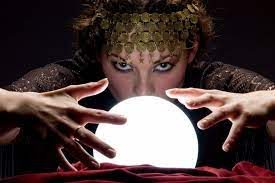
\includegraphics[width=\linewidth]{./IMG-GIT/cristal.jpg}
	\end{center}
\end{center}

\end{multicols}   

\vfill\null
\pagebreak

\begin{center}
	
\includegraphics[height=.7\textheight]{./IMG-GIT/anjo.jpg}
	
		\resizebox{\linewidth}{20mm}{\color{magenta}\textbf{Não tem aula de Informática!}}
\end{center}

   \vfill
\pagebreak

%\begin{center}
%	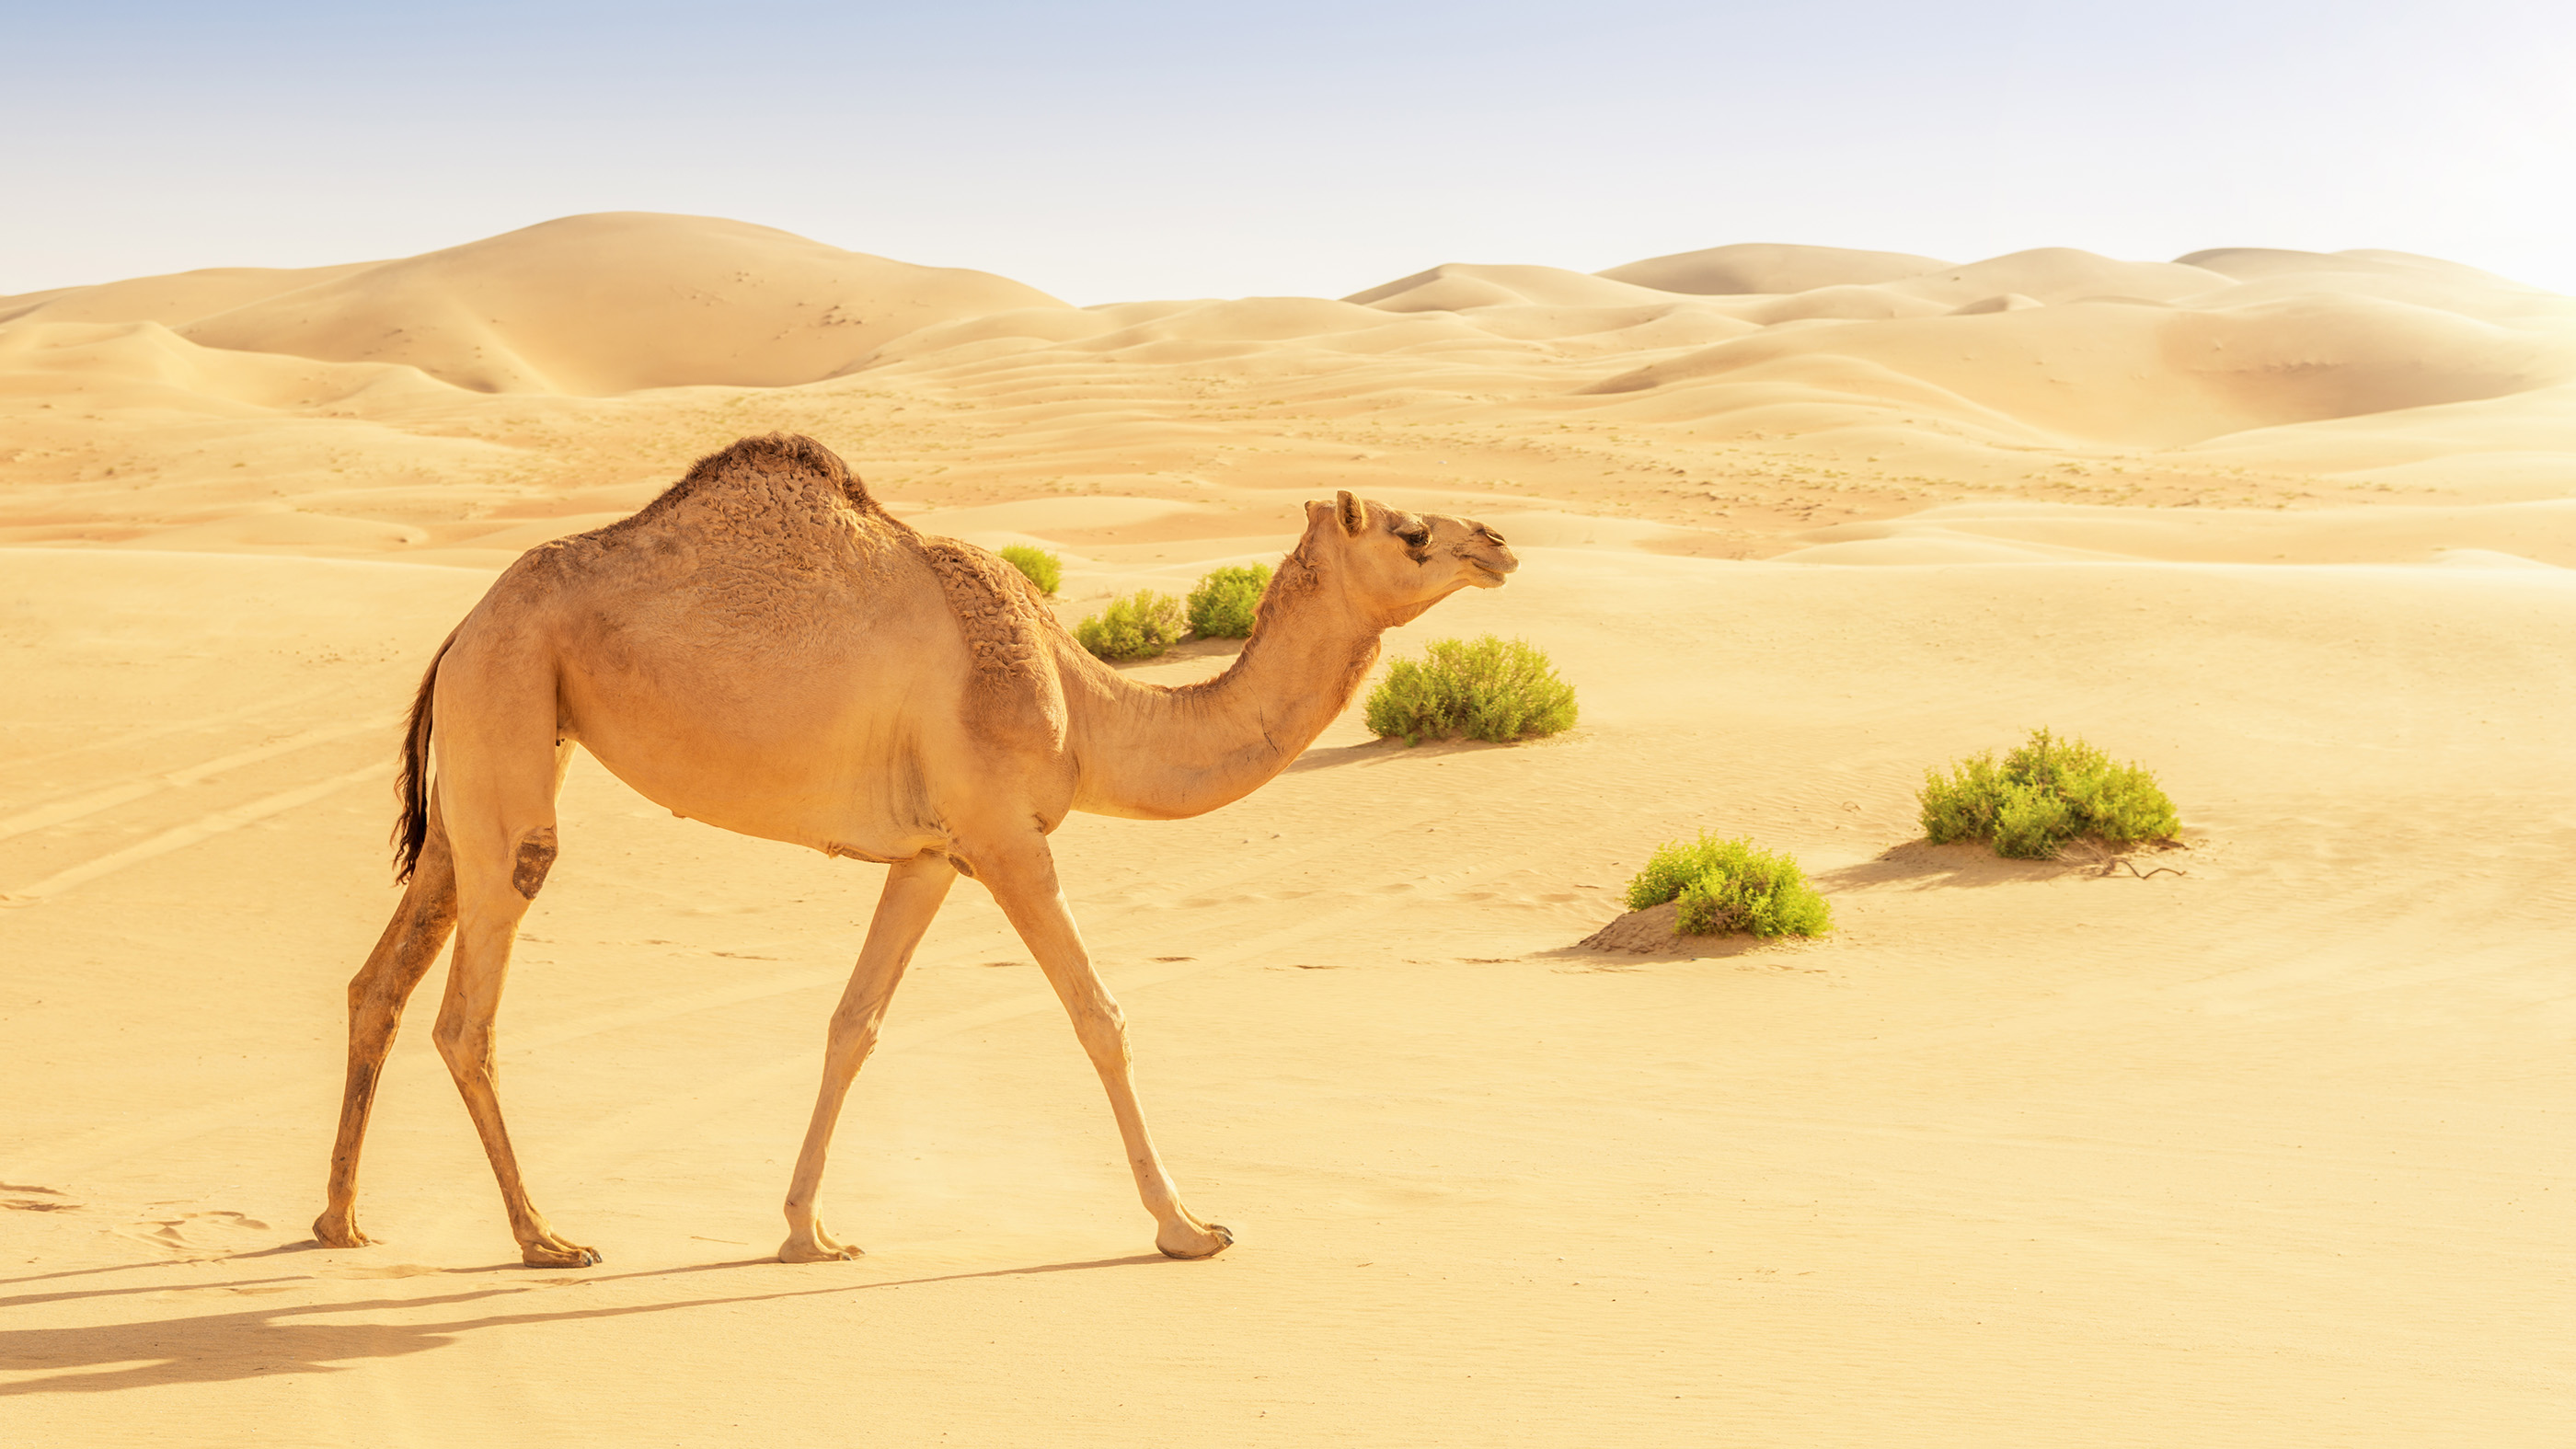
\includegraphics[height=.9\textheight]{./IMG-GIT/camel.jpg}
%\end{center}
%
%   \vfill
%\pagebreak



	\begin{itemize}
		\item  {\LARGE 640 atividades}	
		\item  640 atividades $\ast$ 20 alunos == \textbf{12.800 atividades individuais}.
		\item \textbf{5 linhas de código Shell}
		\item 5 $\ast$ 12.800 == \textbf{64.000} linhas/ano
		\item \textbf{400} linhas/dia
		\item Por escrito.
		\item Em código Shell.
		\item if (hora \textbf{$\geq$ 7:50} da manhã)	
	\end{itemize}

   \vfill
\pagebreak

\vspace*{15mm}
\begin{center}
			\resizebox{.5\linewidth}{.5\textheight}{\color{black}\textbf{8:00}}
\end{center}
		
		   \vfill
		\pagebreak

\ThisCenterWallPaper{1.2}{./IMG-GIT/enchente.jpg}
\begin{center}
	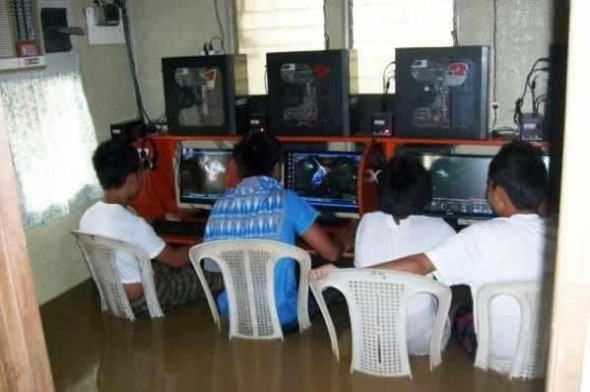
\includegraphics[height=.9\textheight]{./IMG-GIT/enchente.jpg}
\end{center}


\vfill
\pagebreak

\begin{center}
	
\includegraphics[height=.7\textheight]{./IMG-GIT/anjo.jpg}
	
	\resizebox{\linewidth}{20mm}{\color{magenta}\textbf{Não tem aula de Informática!}}
\end{center}

\vfill
\pagebreak


\begin{multicols}{2}
	
	\begin{center}
		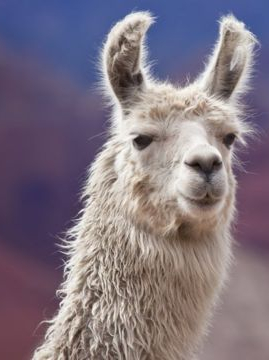
\includegraphics[height=\textheight]{./IMG-GIT/lhama.jpg}
		
		\resizebox{\linewidth}{15mm}{\color{black}\textbf{Lhamento!}}
	\end{center}		
	
	\begin{itemize}
		
		\large
		\item Servico Público.
		\item Jurisprudência.
		\item O que e falado, não tem valor jurídico.
		\item \textbf{Jarvis} não esta previsto no orcamento.
		\item \textbf{Se a Escola não solicitar a atividade, a atividade não foi solicitada!}
		\item Abriu chamado?
		\item Sem "papel", sem atividade!
	\end{itemize}
\end{multicols}

\begin{center}
	\begin{center}
		\LARGE Sua atividade não chegou!
		
		\vspace*{2mm}
		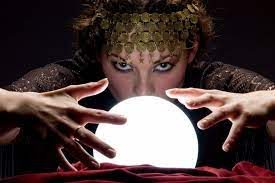
\includegraphics[height=.9\textheight]{./IMG-GIT/cristal.jpg}
	\end{center}
\end{center}

\vfill
\pagebreak

\ThisCenterWallPaper{1}{./IMG-GIT/marvin.jpg}
\LARGE   
\textbf{Planejamento}


	\begin{itemize}
		\Large
		\item \textbf{Projeto Pedagógico}	
		\item Lista de atividades
		\item Descrição de atividades
		\item Cronograma	
		%\begin{itemize}
		%	\LARGE
		%  		\item EF1: 160 atividades
		%  		\item EF2: 128 
		%  		\item EM: 96
		%\end{itemize}
		\item \textbf{Por escrito!}
		\item if (\textbf{!}escrito)
		\subitem \{\textbf{!}programado \&\& {!}executado\}
		%	\subitem \normalsize TEX ou TXT.
	\end{itemize}

	\vfill	
\pagebreak

\begin{center}
	
\includegraphics[height=.7\textheight]{./IMG-GIT/anjo.jpg}
	
	\resizebox{\linewidth}{20mm}{\color{magenta}\textbf{Não tem aula de Informática!}}
	
\end{center}
\vfill
\pagebreak

\begin{multicols}{2}
		
	\begin{flushright}
			{
	\LARGE
	Deseja obter ajuda dos \\Vogons?\\
	{\LARGE Vogosfera Alpa-Centauri\\10 anos luz}
}
	
	
\includegraphics[width=.6\linewidth]{./IMG-GIT/yes-no.png}		
	\end{flushright}	

	\vfill
	\columnbreak
	
	\begin{center}
		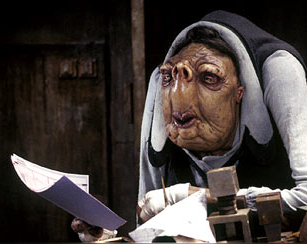
\includegraphics[width=\linewidth]{./IMG-GIT/vogons2.jpg}
\end{center}
\end{multicols}

\begin{frame}
	
	\centering % Para centralizarmos o vídeo
	\includemedia[
	label=nome-qualquer, % ! Importante para linkar o vídeo ao botao (ver abaixo)
	width=0.8\linewidth, height=0.5\linewidth, % Dimensões
	addresource=./MP4-GIT/VOGON.mp4, % ESTE É O SEU ARQUIVO DE VÍDEO (mesmo dir.)
	transparent, % Opcões para que o player tenha transparência
	activate=pageopen, % Se você deseja que o vídeo esteja "carregado" ao abrir a página
	flashvars={
		source=./MP4-GIT/VOGON.mp4
		&loop=false % Se você quer que o vídeo repita automaticamente 
		&scaleMode=letterbox % Manter proporcões (dimensionais) do vídeo
	}
	]{}{./MP4-GIT/VOGON.mp4}
	\vspace{1cm} % Espacamento entre vídeo e botao
	
	% Agora, você cria o botao para dar play/pause. Neste caso, o botao e apenas a letra "pi".
	
%	\mediabutton[
%	mediacommand=nome_qualquer:playPause,
%	overface=\color{black}{{\strut $\pi$}},
%	downface=\color{gray}{{\strut $\pi$}}
%	]{{\strut $\pi$}}
	
	
\end{frame}



\vfill
\pagebreak

\begin{center}
	
\includegraphics[height=.7\textheight]{./IMG-GIT/anjo.jpg}
	
	\resizebox{\linewidth}{20mm}{\color{magenta}\textbf{Continua sem Informática!}}
	
\end{center}

%\vfill
%\pagebreak
%Mas agora tem musiquinha de elevador ou poesia vogon...
%
%Se vc não se importa com oq acontece ao seu redor, o problema e seu!


\vfill
\pagebreak


{\LARGE Deseja tentar outro canal de atendimento?}	

\begin{multicols}{3}	
\begin{center}
	
\includegraphics[height=.5\textheight]{./IMG-GIT/fada.jpeg}
\end{center}
\begin{flushright}
	
\includegraphics[height=20mm]{./IMG-GIT/whatsapp.png}
\end{flushright}

\vfill	
\columnbreak

\begin{center}
	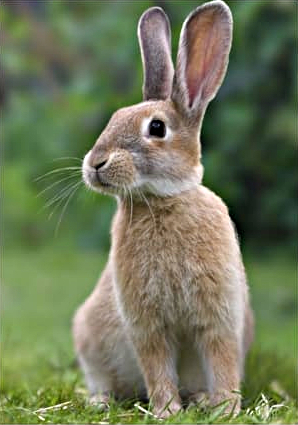
\includegraphics[height=.5\textheight]{./IMG-GIT/coelhinho.jpeg}
\end{center}
\begin{flushright}
	
\includegraphics[height=20mm]{./IMG-GIT/whatsapp.png}
\end{flushright}

	\vfill	
	\columnbreak

\begin{center}
	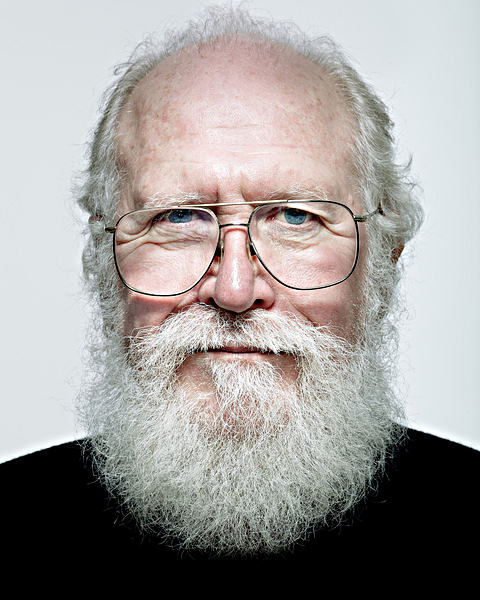
\includegraphics[height=.5\textheight]{./IMG-GIT/maddog.jpg}
\end{center}
\begin{flushright}
	
\includegraphics[height=20mm]{./IMG-GIT/whatsapp.png}
\end{flushright}
\end{multicols}	

\vfill
\pagebreak

    \ThisCenterWallPaper{1}{./IMG-GIT/ANDROMEDA.jpg}
    
\begin{multicols}{2}    
\begin{center}
	\includegraphics[height=1.15\textheight]{./IMG-GIT/lhama.png}
	
%\vspace*{-5mm}
\vfil
\columnbreak

	\resizebox{\linewidth}{15mm}{\color{white}\textbf{Lhamento!}}

%\vspace*{-15mm}	
	{\color{white}\LARGE É assim que computadores funcionam !}
\end{center}

\begin{flushright}	
	{\color{white}
		\Large
		Deseja reiniciar o Universo?
		
		\includegraphics[width=.6\linewidth]{./IMG-GIT/yes-no.png}		
	}
\end{flushright}
\vfill
\end{multicols}


\pagebreak

 \ThisCenterWallPaper{1.05}{./IMG-GIT/spacex.jpg}

{\LARGE \color{white}Aproveite a viagem!}
	
	\vfill
	\pagebreak	
	
	\ThisCenterWallPaper{1.05}{./IMG-GIT/spacex.jpg}
	
	{\LARGE \color{white}Não esqueca sua toalha!}
		
\vfill
\pagebreak

\ThisCenterWallPaper{1}{./IMG-GIT/PALESTRANTES/flisol-latino.jpg}

{\huge Não entre em pânico!}

\vfill
\pagebreak
%\begin{multicols}{3}
%	
%	\begin{center}
%		\includegraphics[width=\linewidth]{./IMG-GIT/PALESTRANTES/julio.jpg}
%
%	\includegraphics[width=\linewidth]{./IMG-GIT/PALESTRANTES/junit.jpg}
%
%	\includegraphics[width=\linewidth]{./IMG-GIT/PALESTRANTES/ole.jpg}
%
%	\includegraphics[width=\linewidth]{./IMG-GIT/PALESTRANTES/pedrohenriquefreecad.jpg}
%	
%	\includegraphics[width=\linewidth]{./IMG-GIT/PALESTRANTES/bispo.jpg}
%	
%	\includegraphics[width=\linewidth]{./IMG-GIT/PALESTRANTES/mazoni.jpg}
%
%\end{center}
%
%\end{multicols}

\vfill
\pagebreak

%\ThisCenterWallPaper{1}{./IMG-GIT//PALESTRANTES/aravecchia.jpg}
%
%\vfill
%\pagebreak

\ThisCenterWallPaper{1}{./IMG-GIT/SVG/DIAGRAMAS10.png}

\vspace*{.75\textheight}
{\Huge Efestus}
 \vfill
\pagebreak


%\ThisCenterWallPaper{1}{./IMG-GIT/marvin.jpg}
%
%\vspace*{2mm}
%\begin{minipage}{\linewidth}
%	\begin{minipage}[c]{0.5\linewidth}
%		
%\begin{center}
%		\includegraphics[width=\linewidth]{./IMG-GIT/CAPA.png}
%		
%		{\LARGE 15 de abril}
%		
%%				\includegraphics[width=.5\linewidth]{./IMG-GIT/flisol-logo.jpg}
%				
%			\resizebox{.7\linewidth}{8mm}{\color{black}sugep.ifg.edu.br}
%\end{center}
%	\end{minipage}
%	\begin{minipage}[t]{0.3\linewidth}
%%		Conteúdo da segunda minipage
%	\end{minipage}
%\end{minipage}
% 
\vfill
\pagebreak

\ThisCenterWallPaper{1}{./IMG-GIT/dontpanic.jpg}

	\Large
	
\begin{enumerate}
	\item Computadores são mais inteligentes que vogons!
	\item Armazenam e processam uma quantidade absurdamente maior de \nobreak documentos!
	\item Sao absurdamente mais rápidos!
	\item Sao honestos, confiaveis e precisos!
	\item Escrevem poesias melhores.
\end{enumerate}
	
	\vfill
	\pagebreak	
	
\begin{multicols}{2}
	\Huge Planejamento

\vfill\null
\columnbreak

			\includepdf[pages=1,height=1.5\textheight]{./PDF-GIT/RESOLUCAO-001_22.pdf}
		
\end{multicols}
		\vfill
		\pagebreak

\begin{center}
			\includegraphics[height=\textheight]{./IMG-GIT/ano-1-e-2.jpeg}
\end{center}


\vfill
\pagebreak


\begin{multicols}{2}
	
\begin{itemize}	
\Large \item \textbf{Secretaria de Educação}
\item\textbf{Escola}

\large
\begin{itemize}
 	\item Direção
	\item Coordenação
	\item Conselho
\end{itemize}


\large	\item \textbf{Lista de atividades}:
\begin{itemize}
	\item EF1: 160 
	\item EF2: 128
	\item EM: 96 atividades.
\end{itemize}
\end{itemize}

\vfill\null
\columnbreak

\Large
	\begin{enumerate}
		\item Descrição sumaria da atividade
		\item Recurso computacional desejado
\begin{itemize}
		\item Texto
\begin{itemize}
	\large \item Links
	\item Aplicativos
\end{itemize}
	\item Documentos anexos:
	\begin{itemize}
		\large \item imagens
		\item videos
		\item arquivos
		\item slides
		\item musica
	\end{itemize} 
\end{itemize}
	\end{enumerate}

\vfill\null
\columnbreak

\Large
	\textbf{Laboratório de Informática}:

\begin{itemize}
	\Large
	\item \textbf{Servidor}:
	\Large 	\begin{enumerate}
\item Incorporar a Lista de Atividades ao MAIN.tex
		\item Gerar PDF com \LaTeX.
		\item Exportar de hora em hora para \textit{index.html}.
	\end{enumerate}

\vfill\null
\columnbreak

\Large
\item \textbf{Cliente}:
	\begin{enumerate}
\Large
	\item Inicialização automática do usuario aluno.
	\item Inicialização automática do navegador.
	\item Página inicial no \href{www.localhost}{\textbf{servidor}}.
	\vfill\null
	\columnbreak
		\item Diversão:
\begin{itemize}
	 \large
	 \item Scripts diversos.
	\item Acesso remoto: SSH.
	\item Horarios: \textbf{crontab}.	
	\item Liberar INDEX.html local para os alunos.
	\item Sistema de log.
	\item Gamificação.
	\item ...
\end{itemize}
\end{enumerate}
\end{itemize}
   
   \vfill\null
   \columnbreak
   
   \begin{center}
   	\includegraphics[height=.7\textheight]{./IMG-GIT/linus.jpeg}
   \end{center}

\Large \begin{enumerate}
	\item Não fale.
\item Mostre o código
\end{enumerate}

\end{multicols}

\vfill\null
\pagebreak






\color{black}
\begin{multicols}{2}
\chapter[ 1\textordmasculine\space Ano: o Be-A-Bá]{1\textordmasculine\space Ano: o Be-A-Bá}

%  \addcontentsline{toc}{chapter}{Capitulo Não Numerado} % Linha para adicionar o item ao sumario.
\pagebreak

%\begin{center}
%	\includegraphics[width=\linewidth]{./IMG/codigos-bncc.png}
%\end{center}
%
%\pagebreak
%
%\includepdf[scale=1.1,pages=35]{BNCC-Tecnologia.pdf}
%
%\pagebreak
%
%\begin{center}
%	\includegraphics[height=\textheight]{./IMG/ano-1-e-2.jpeg}
%\end{center}
%
%\pagebreak
%
%\includepdf[scale=1,pages=30-36,angle=90]{CIEB.pdf}

\pagebreak

	\section[\sffamily 1\textordmasculine\space Ano - Mês 1 - Aula-1]{\sffamily 1\textordmasculine\space Ano - Mês 1 - Aula-1}

\ClearWallPaper % Limpa o papel de parede para evitar sobreposição

\normalsize

\begin{enumerate}
	\item Apresentação do Laboratório
	\begin{enumerate}
		\item Verificar o grau de maturidade dos alunos, quanto à segurança.
		\item Verificar a famíliaridade dos alunos quanto ao uso da tecnologia, no dia-a-dia.
		\item Deixar a criança se habituar ao espaco físico.
		\item Explicar claramente as regras do Laboratório (exercitadas por meio de \textbf{killall -u user}).
		\begin{enumerate}
			\item Não correr \textbf{nunca}.
			\item Não trazer agua ou comida para o Laboratório.
			\item Andar devagar e pensar rápido.
			\item Bagunça \textbf{zero}.
		\end{enumerate}
	\item Explicar exaustivamente as razões de segurança: \textbf{corta, da choque, pega fogo}.
	\item Alguem ja colocou o dedo na tomada?
	\end{enumerate}
\item Tomada, fonte e bateria: muita energia e pouca energia.
\begin{enumerate}
	\item Experimento com tomada, lampada e fio desencapado.
	\item Experimento com bateria $4.5V$, Led, resistor de 360$\Omega$.
	\item Experimento com fonte $5V$, Led, resistor de 360$\Omega$.
\end{enumerate}
\item Conceitos:
\begin{enumerate}
	\item SIM $\|$ NÃO.
	\item Ligado $\|$ desligado.
	\item Aceso $\|$ apagado.
	\item 0 $\|$ 1
	\item perigo $\|$ \textbf{!} perigo.
\end{enumerate}
\end{enumerate}



\section[\sffamily 1\textordmasculine\space Ano - Mês 1 - Aula-2]{\sffamily 1\textordmasculine\space Ano - Mês 1 - Aula-2}
\begin{enumerate}
	\item Primeiro contato com o computador.
	\begin{enumerate}
		\item Componentes básicos:
		\begin{enumerate}
			\item Tomada.
			\item Estabilizador.
			\item Computador, gabinete, torre: !CPU.
			\item Video.
			\item Teclado.
			\item Mouse (colar olhos, orelhas, focinho e bigode no rato).
			\item \textbf{Software}: deve ser chamado de \textbf{programa}, nesta idade.
		\end{enumerate}
	\item Avaliação psico-motora. \href{https://studio.code.org/s/pre-express-2023/lessons/1/levels/1?lang=pt-BR}{Clicar, arrastar e soltar.}.
	\begin{enumerate}
		\item Sequencialidade.
		\item Reconhecimento de formas.
		\item Reconhecimento de cores.
		\item Agrupamento.
		\item Lateralidade.
		\item Espacialidade.
		\item Coordenação motora.
		\item Habilidades psico-motoras.
	\end{enumerate}
	\end{enumerate}
\end{enumerate}



\section[\sffamily 1\textordmasculine\space Ano - Mês 1 - Aula-3]{\sffamily 1\textordmasculine\space Ano - Mês 1 - Aula-3}
\href{https://studio.code.org/s/pre-express-2023/lessons/1/levels/1?lang=pt-BR}{Clicar, arrastar e soltar.}

\section[\sffamily 1\textordmasculine\space Ano - Mês 1 - Aula-4]{\sffamily 1\textordmasculine\space Ano - Mês 1 - Aula-4}
\href{https://studio.code.org/s/pre-express-2023/lessons/1/levels/1?lang=pt-BR}{Clicar, arrastar e soltar.}

\section[\sffamily 1\textordmasculine\space Ano - Mês 1 - Aula-5]{\sffamily 1\textordmasculine\space Ano - Mês 1 - Aula-5}
\href{https://studio.code.org/s/pre-express-2023/lessons/2/levels/1?lang=pt-BR}{Sequenciamento e lateralidade.}


\section[\sffamily 1\textordmasculine\space Ano - Mês 1 - Aula-6]{\sffamily 1\textordmasculine\space Ano - Mês 1 - Aula-6}
\href{https://studio.code.org/s/pre-express-2023/lessons/2/levels/1?lang=pt-BR}{Sequenciamento e lateralidade.}


\section[\sffamily 1\textordmasculine\space Ano - Mês 2 - Aula-3]{\sffamily 1\textordmasculine\space Ano - Mês 2 - Aula-3}
\href{https://studio.code.org/s/pre-express-2023/lessons/3/levels/2?lang=pt-BR}{Sequenciamento e lateralidade.}

\section[\sffamily 1\textordmasculine\space Ano - Mês 2 - Aula-4]{\sffamily 1\textordmasculine\space Ano - Mês 2 - Aula-4}
\href{https://studio.code.org/s/pre-express-2023/lessons/3/levels/2?lang=pt-BR}{Sequenciamento e lateralidade.}

\section[\sffamily 1\textordmasculine\space Ano - Mês 3 - Aula-1]{\sffamily 1\textordmasculine\space Ano - Mês 3 - Aula-1}
\begin{enumerate}
	\item \url{run:./frozen-bubble.lnk}
	\item  \href{run:./frozen-bubble.lnk}{Frozen Buble}.
	\begin{enumerate}
		\item Avaliação gamificada.
		\item Sequencialidade.
		\item Reconhecimento de formas.
		\item Reconhecimento de cores.
		\item Reconhecimento de padrões.
		\item Lateralidade.
		\item Espacialidade.
		\item Coordenação motora.
		\item Habilidades psico-motoras.
	\end{enumerate}
\end{enumerate}


\section[\sffamily 1\textordmasculine\space Ano - Mês 3 - Aula-2]{\sffamily 1\textordmasculine\space Ano - Mês 3 - Aula-2}
\begin{enumerate}
	\item Frozen Buble.
	\begin{enumerate}
		\item Avaliação gamificada.
		\item Sequencialidade.
		\item Reconhecimento de formas.
		\item Reconhecimento de cores.
		\item Reconhecimento de padrões.
		\item Lateralidade.
		\item Espacialidade.
		\item Coordenação motora.
		\item Habilidades psico-motoras.
	\end{enumerate}
\end{enumerate}

\section[\sffamily 1\textordmasculine\space Ano - Mês 3 - Aula-3]{\sffamily 1\textordmasculine\space Ano - Mês 3 - Aula-3}
\begin{enumerate}
	\item Frozen Buble.
	\begin{enumerate}
		\item Avaliação gamificada.
		\item Sequencialidade.
		\item Reconhecimento de formas.
		\item Reconhecimento de cores.
		\item Reconhecimento de padrões.
		\item Lateralidade.
		\item Espacialidade.
		\item Coordenação motora.
		\item Habilidades psico-motoras.
	\end{enumerate}
\end{enumerate}

\section[\sffamily 1\textordmasculine\space Ano - Mês 3 - Aula-4]{\sffamily 1\textordmasculine\space Ano - Mês 3 - Aula-4}
\begin{enumerate}
	\item Frozen Buble.
	\begin{enumerate}
		\item Avaliação gamificada.
		\item Sequencialidade.
		\item Reconhecimento de formas.
		\item Reconhecimento de cores.
		\item Reconhecimento de padrões.
		\item Lateralidade.
		\item Espacialidade.
		\item Coordenação motora.
		\item Habilidades psico-motoras.
	\end{enumerate}
\end{enumerate}

\section[\sffamily 1\textordmasculine\space Ano - Mês 4 - Aula-1]{\sffamily 1\textordmasculine\space Ano - Mês 4 - Aula-1}
\begin{itemize}
	\item Lógica de interface gráfica.
	\item Colaboração mútua.
	\item Auto-imagem.
	\item Auto-confiança, no uso de novas ferramentas.
	\item Criatividade no meio digital.
	\item Observar:
	\begin{itemize}
		\item Agrupamentos entre alunos.
		\item Sinais comportamentais, expressos no cenario virtual criado pelo aluno.
		\item Interesses individuais e coletivos, em função dos cenários escolhidos pelos alunos.
		\item Sinais de eventuais problemas cognitivos, psicológicos ou famíliares.
	\end{itemize}
\end{itemize}

\section[\sffamily 1\textordmasculine\space Ano - Mês 4 - Aula-2]{\sffamily 1\textordmasculine\space Ano - Mês 4 - Aula-2}
\begin{itemize}
	\item Kapman
	\begin{itemize}
		\item Habilidades psico-motoras sob pressão do jogo.
		\item Lateralidade.
		\item Espacialidade.
	\end{itemize}
\end{itemize}


\section[\sffamily 1\textordmasculine\space Ano - Mês 4 - Aula-3]{\sffamily 1\textordmasculine\space Ano - Mês 4 - Aula-3}
\begin{enumerate}
	\item Escolha: Homem Batata \textbf{$\Vert$} Kapman.
	\begin{enumerate}
		\item Observar a escolha individual de meninos e meninas.
		\item Observar agrupamentos entre alunos.
		\item Incentivar a colaboração mútua.
	\end{enumerate}
\end{enumerate}

\section[\sffamily 1\textordmasculine\space Ano - Mês 4 - Aula-4]{\sffamily 1\textordmasculine\space Ano - Mês 4 - Aula-4}
\begin{enumerate}
	\item Escolha: Homem Batata $\|$ Kapman.
	\begin{enumerate}
		\item Observar a escolha individual de meninos e meninas.
		\item Observar agrupamentos entre alunos.
		\item Incentivar a colaboração mútua.
	\end{enumerate}
\end{enumerate}


\section[\sffamily 1\textordmasculine\space Ano - Mês 5 - Aula-1]{\sffamily 1\textordmasculine\space Ano - Mês 5 - Aula-1}
\begin{itemize}
	\item Tuxpaint.
	\begin{itemize}
		\item Ícones: associação de ideias a palavras e formas geométricas.
		\item Símbolos: (\textit{sym boulos}?)
		\item Formas geométricas.
		\item Cores.
		\item Sequências de comandos: ceu. lua e estrelas.
		\item Configuracões.
	\end{itemize}
\end{itemize}


\section[\sffamily 1\textordmasculine\space Ano - Mês 5 - Aula-2]{\sffamily 1\textordmasculine\space Ano - Mês 5 - Aula-2}
\begin{itemize}
	\item Frozen Bubble.
\end{itemize}


\section[\sffamily 1\textordmasculine\space Ano - Mês 5 - Aula-3]{\sffamily 1\textordmasculine\space Ano - Mês 5 - Aula-3}
\begin{itemize}
	\item Frozen Bubble.
\end{itemize}


\section[\sffamily 1\textordmasculine\space Ano - Mês 5 - Aula-4]{\sffamily 1\textordmasculine\space Ano - Mês 5 - Aula-4}
\begin{itemize}
	\item Frozen Bubble.
\end{itemize}


\section[\sffamily 1\textordmasculine\space Ano - Mês 6 - Aula-1]{\sffamily 1\textordmasculine\space Ano - Mês 6 - Aula-1}
\begin{itemize}
	\item Gcompriz.
	\begin{enumerate}
		\item Explicar a lógica de interfaces:
		\begin{enumerate}
			\item Ícones e associação de idéias.
			\item Árvore.
			\item Menu principal: avanço e retrocesso (uma formiguinha andando numa árvore).
	\item Janelas.
%				\item Botões: \textbf{$\_ \Square \boxtimes$}.
		\end{enumerate}
	\item Observar agrupamentos de alunos.
	\item Incentivar a colaboração mútua.
	\item Incentivar o compartilhamento de idéias e informações.
	\item Incentivar a livre exploração do software.
	\end{enumerate}
\end{itemize}

\section[\sffamily 1\textordmasculine\space Ano - Mês 6 - Aula-2]{\sffamily 1\textordmasculine\space Ano - Mês 6 - Aula-2}
\begin{itemize}
	\item GCompriz
\end{itemize}


\section[\sffamily 1\textordmasculine\space Ano - Mês 6 - Aula-3]{\sffamily 1\textordmasculine\space Ano - Mês 6 - Aula-3}
\begin{itemize}
	\item GCompriz
\end{itemize}



\section[\sffamily 1\textordmasculine\space Ano - Mês 6 - Aula-4]{\sffamily 1\textordmasculine\space Ano - Mês 6 - Aula-4}
\begin{itemize}
	\item GCompriz
\end{itemize}


\section[\sffamily 1\textordmasculine\space Ano - Mês 7 - Aula-1]{\sffamily 1\textordmasculine\space Ano - Mês 7 - Aula-1}
\href{https://studio.code.org/s/pre-express-2023/lessons/3/levels/2?lang=pt-BR}{Sequenciamento, lateralidade e iteração.}


\section[\sffamily 1\textordmasculine\space Ano - Mês 7 - Aula-2]{\sffamily 1\textordmasculine\space Ano - Mês 7 - Aula-2}
\href{https://studio.code.org/s/pre-express-2022/lessons/3/levels/2?lang=pt-BR}{Sequenciamento e iteração.}


\section[\sffamily 1\textordmasculine\space Ano - Mês 7 - Aula-3]{\sffamily 1\textordmasculine\space Ano - Mês 7 - Aula-3}
\href{https://studio.code.org/s/pre-express-2023/lessons/4/levels/2?lang=pt-BR}{Sequenciamento e iteração.}

\section[\sffamily 1\textordmasculine\space Ano - Mês 7 - Aula-4]{\sffamily 1\textordmasculine\space Ano - Mês 7 - Aula-4}
\href{https://studio.code.org/s/pre-express-2023/lessons/4/levels/2?lang=pt-BR}{Sequenciamento e iteração.}

\section[\sffamily 1\textordmasculine\space Ano - Mês 8 - Aula-1]{\sffamily 1\textordmasculine\space Ano - Mês 8 - Aula-1}
\href{https://studio.code.org/s/pre-express-2022/lessons/5/levels/2?lang=pt-BR}{Programação de eventos.}


\section[\sffamily 1\textordmasculine\space Ano - Mês 8 - Aula-2]{\sffamily 1\textordmasculine\space Ano - Mês 8 - Aula-2}
\href{https://studio.code.org/s/pre-express-2022/lessons/5/levels/2?lang=pt-BR}{Programação de eventos.}


\section[\sffamily 1\textordmasculine\space Ano - Mês 8 - Aula-3]{\sffamily 1\textordmasculine\space Ano - Mês 8 - Aula-3}
\href{https://studio.code.org/s/pre-express-2023/lessons/5/levels/2?lang=pt-BR}{Programação de eventos.}


\section[\sffamily 1\textordmasculine\space Ano - Mês 8 - Aula-4]{\sffamily 1\textordmasculine\space Ano - Mês 8 - Aula-4}
\href{https://studio.code.org/s/pre-express-2023/lessons/5/levels/2?lang=pt-BR}{Programação de eventos.}

\vfill\null
\pagebreak

%\CenterWallPaper{1}{./IMG-GIT/younglings.jpeg}

\end{multicols}



	\chapter[ 2\textordmasculine\space Ano: o ABC]{2\textordmasculine\space Ano: o ABC}

\includepdf[scale=1.1,pages=36]{BNCC-Tecnologia.pdf}


\pagebreak

\begin{center}
	\includegraphics[height=\textheight]{./IMG/ano-1-e-2.jpeg}
\end{center}

\pagebreak

%\includepdf[scale=1,pages=37-44,angle=90]{CIEB.pdf}
\normalsize


Nota: pelas características do público atendido pela escola, e por razões técnico-pedagógicas, pesquisas na Internet serao realizadas a partir do 3\textordmasculine\space ano, e  4\textordmasculine\space anos,  quando os alunos terão mais maturidade e conhecimento no uso do desktop.

\begin{multicols}{2}
\section[\sffamily 2\textordmasculine\space Ano - Mês 1 - Aula-1]{\sffamily 2\textordmasculine\space Ano - Mês 1 - Aula-1}
\begin{enumerate}
	\item Área de trabalho GNU-Linux.
	\begin{enumerate}
		\item Tela.
		\item Barra de ferramentas.
		\item Menu iniciar.
		\begin{enumerate}
			\item Menu de aplicativos (botão Iniciar): conceito básico de raiz/árvore Unix.
			\item Uma formiguinha caminhando pelos galhos de uma árvore.
			\item Conceito de comando.
			\item Atalho Alt-F2 (comparar clique do mouse ao botão Enter).
			\item Atalho Alt-F4.
		\end{enumerate}
	\item Exploração livre dos aplicativos.
	\begin{enumerate}
		\item Habilidades psico-motoras.
		\item Estimular a leitura.
		\item Lógica básica de navegação em um ambiente X.
		\item Observar o interesse dos alunos por cada aplicativo que escolherem.
	\end{enumerate}
	\end{enumerate}
\end{enumerate}


\section[\sffamily 2\textordmasculine\space Ano - Mês 1 - Aula-2]{\sffamily 2\textordmasculine\space Ano - Mês 1 - Aula-2}
\begin{itemize}
	\item Livre exploração da área de trabalho, menu iniciar e aplicativos.
	\item Incentivar o uso dos atalhos Alt-F2 e Alt-F4.
%	\item Botões: \textbf{$\_ \boxtimes \boxtimes$}.
\end{itemize}


\section[\sffamily 2\textordmasculine\space Ano - Mês 1 - Aula-3]{\sffamily 2\textordmasculine\space Ano - Mês 1 - Aula-3}
\begin{itemize}
	\item Livre exploração da area de trabalho, menu iniciar e aplicativos.
	\item Incentivar o uso dos atalhos Alt-F2 e Alt-F4.
%	\item Botões: \textbf{$\_ \boxtimes \boxtimes$}.
\end{itemize}



\section[\sffamily 2\textordmasculine\space Ano - Mês 1 - Aula-4]{\sffamily 2\textordmasculine\space Ano - Mês 1 - Aula-4}
\begin{itemize}
	\item Livre exploração da área de trabalho, menu iniciar e aplicativos.
	\item Incentivar o uso dos atalhos Alt-F2 e Alt-F4.
%	\item Botões: \textbf{$\_ \boxtimes \boxtimes$}.
\end{itemize}



\section[\sffamily 2\textordmasculine\space Ano - Mês 2 - Aula-1]{\sffamily 2\textordmasculine\space Ano - Mês 2 - Aula-1}
\href{https://studio.code.org/s/pre-express-2022/lessons/5/levels/2}{Programação de eventos}.



\section[\sffamily 2\textordmasculine\space Ano - Mês 2 - Aula-2]{\sffamily 2\textordmasculine\space Ano - Mês 2 - Aula-2}
\href{https://studio.code.org/s/pre-express-2022/lessons/5/levels/2}{Programação de eventos}.


\section[\sffamily 2\textordmasculine\space Ano - Mês 2 - Aula-3]{\sffamily 2\textordmasculine\space Ano - Mês 2 - Aula-3}
\href{https://studio.code.org/s/pre-express-2022/lessons/5/levels/2}{Programação de eventos}.



\section[\sffamily 2\textordmasculine\space Ano - Mês 2 - Aula-4]{\sffamily 2\textordmasculine\space Ano - Mês 2 - Aula-4}
\href{https://studio.code.org/s/pre-express-2022/lessons/5/levels/2}{Programação de eventos}.



\section[\sffamily 2\textordmasculine\space Ano - Mês 3 - Aula-1]{\sffamily 2\textordmasculine\space Ano - Mês 3 - Aula-1}
\href{https://studio.code.org/s/pre-express-2022/lessons/5/levels/2}{Programação de eventos}.



\section[\sffamily 2\textordmasculine\space Ano - Mês 3 - Aula-2]{\sffamily 2\textordmasculine\space Ano - Mês 3 - Aula-2}
\href{https://studio.code.org/s/pre-express-2022/lessons/5/levels/2}{Programação de eventos}.


\section[\sffamily 2\textordmasculine\space Ano - Mês 3 - Aula-3]{\sffamily 2\textordmasculine\space Ano - Mês 3 - Aula-3}
\href{https://studio.code.org/s/pre-express-2022/lessons/5/levels/2}{Programação de eventos}.


\section[\sffamily 2\textordmasculine\space Ano - Mês 3 - Aula-4]{\sffamily 2\textordmasculine\space Ano - Mês 3 - Aula-4}
\href{https://studio.code.org/s/pre-express-2022/lessons/5/levels/2}{Programação de eventos}.


\section[\sffamily 2\textordmasculine\space Ano - Mês 4 - Aula-1]{\sffamily 2\textordmasculine\space Ano - Mês 4 - Aula-1}
\href{https://studio.code.org/s/pre-express-2022/lessons/7/levels/1}{Programação de eventos}.


\section[\sffamily 2\textordmasculine\space Ano - Mês 4 - Aula-2]{\sffamily 2\textordmasculine\space Ano - Mês 4 - Aula-2}
\href{https://studio.code.org/s/pre-express-2022/lessons/7/levels/1}{Programação de eventos}.


\section[\sffamily 2\textordmasculine\space Ano - Mês 4 - Aula-3]{\sffamily 2\textordmasculine\space Ano - Mês 4 - Aula-3}
\begin{center}
	\includegraphics[width=\linewidth]{./IMG/Screenshot_20221101_090407.png}
\end{center}

\begin{itemize}
	\item \textbf{KolourPaint}.
	\item Exercitar o uso de ícones
	\item Botões em geral
	\item Analogia de ideias
	\item Sequenciamento lógico.
	\item Ressaltar as equivalências e diferencas entre mundo físico e mundo virtual.
	\item Pincel $\Rightarrow$ Cor $\Rightarrow$ Papel $\Rightarrow$ Apertar o lapis (click) $\Rightarrow$ Arrastar $\Rightarrow$ Soltar
\end{itemize}



\section[\sffamily 2\textordmasculine\space Ano - Mês 4 - Aula-4]{\sffamily 2\textordmasculine\space Ano - Mês 4 - Aula-4}
\begin{itemize}
	\item KolourPaint.
	\item Exercitar o uso de ícones e botões em geral, através de sequenciamento lógico.
	\item Ressaltar as equivalências e diferenças entre mundo físico e mundo virtual.
	\item Pincel $\Rightarrow$ Cor $\Rightarrow$ Papel $\Rightarrow$ Apertar o lápis (click) $\Rightarrow$ Arrastar $\Rightarrow$ Soltar
\end{itemize}

\section[\sffamily 2\textordmasculine\space Ano - Mês 5 - Aula-1]{\sffamily 2\textordmasculine\space Ano - Mês 5 - Aula-1}
\begin{itemize}
	\item KolourPaint.
	\item Exercitar o uso de ícones e botões em geral, através de sequenciamento lógico.
	\item Ressaltar as equivalências e diferencas entre mundo físico e mundo virtual.
	\item Pincel $\Rightarrow$ Cor $\Rightarrow$ Papel $\Rightarrow$ Apertar o lapis (click) $\Rightarrow$ Arrastar $\Rightarrow$ Soltar
\end{itemize}

\section[\sffamily 2\textordmasculine\space Ano - Mês 5 - Aula-2]{\sffamily 2\textordmasculine\space Ano - Mês 5 - Aula-2}
\begin{itemize}
	\item \textbf{KolourPaint}.
	\item Exercitar o uso de ícones e botões em geral, através de sequenciamento lógico.
	\item Ressaltar as equivalências e diferencas entre mundo físico e mundo virtual.
	\item Pincel $\Rightarrow$ Cor $\Rightarrow$ Papel $\Rightarrow$ Apertar o lapis (click) $\Rightarrow$ Arrastar $\Rightarrow$ Soltar
\end{itemize}

\section[\sffamily 2\textordmasculine\space Ano - Mês 5 - Aula-3]{\sffamily 2\textordmasculine\space Ano - Mês 5 - Aula-3}
\begin{enumerate}
	\item Digitação com OOo4Kids.
	\begin{enumerate}
		\item asdfg
		\item çlkjh
	\end{enumerate}
\end{enumerate}



\section[\sffamily 2\textordmasculine\space Ano - Mês 5 - Aula-4]{\sffamily 2\textordmasculine\space Ano - Mês 5 - Aula-4}
\begin{enumerate}
	\item Digitação com OOo4Kids.
	\begin{enumerate}
		\item qwerty
		\item poiuy
	\end{enumerate}
\end{enumerate}



\section[\sffamily 2\textordmasculine\space Ano - Mês 6 - Aula-1]{\sffamily 2\textordmasculine\space Ano - Mês 6 - Aula-1}
\begin{enumerate}
	\item Digitação com OOo4Kids.
	\begin{enumerate}
		\item zxcvb
		\item ;.,mn
	\end{enumerate}
\end{enumerate}



\section[\sffamily 2\textordmasculine\space Ano - Mês 6 - Aula-2]{\sffamily 2\textordmasculine\space Ano - Mês 6 - Aula-2}
\begin{enumerate}
	\item Digitação com OOo4Kids.
	\begin{enumerate}
		\item Ditado simples \textbf{sem} em uso de caracteres especiais.
		\item Teclas:
		\begin{enumerate}
			\item Espaco.
			\item Enter.
			\item Cursores \textbf{$\Uparrow\Downarrow\Leftarrow\Rightarrow$}.
			\item Shitf.
			\item Caps Lock.
		\end{enumerate}
	\end{enumerate}
\end{enumerate}


\section[\sffamily 2\textordmasculine\space Ano - Mês 6 - Aula-3]{\sffamily 2\textordmasculine\space Ano - Mês 6 - Aula-3}
\begin{enumerate}
	\item Emojis, emoticons e caracteres especiais.
	\begin{enumerate}
		\item Trabalar lógica do teclado, especialmente a tecla \textbf{Shift}.
		\item Sondar respostas emocionais dos alunos, aos mais variados sentimentos.
		\begin{enumerate}
			\item Filmar a aula, dentro do possível, e gravar eventuais respostas de linguagem corporal, que posso indicar abusos, vulnerabilidade, situação de risco ou dificuldades de aprendizado.
		\end{enumerate} 
		\item Incentivar os alunos a racionalizar sentimentos e traduzi-los de forma iconográfica.
		\item Emojis:
		\begin{enumerate}
			\item :) feliz
			\item :D muito feliz
			\item n\_n sorrindo
			\item \textasciicircum\_\textasciicircum sorrindo
			\item
			\textasciicircum\-\textasciicircum \space sorrindo
			\item :] robô feliz
			\item :( triste
			\item :[ robô triste
			\item :'( muito triste
			\item ;\_; chorando muito
			\item ;O; chorando desesperado(a)mente
			\item :| só observo
			\item :/ desconfiado
			\item :\ Mehh
			\item :* beijo
			\item :*** muitos beijos
			\item <3 coração, amor, amei
			\item :P mostrando a língua
			\item O.o :o impressionado
			\item O\_O maravilhado
			\item o\_o serio?
			\item u\_u com sono ou triste
			\item BD B) "mitando" (eu sou demais)
			\item @-@ nerd
			\item >:( bravo
			\item >:) mau
			\item >:D risada do gênio do mal
			\item '-' inocente, não sei de nada, ou só observo
			\item ;) piscando
			\item 3:-) demônio
			\item x.x morto
			\item o~o louco
			\item -\_- cansado
			\item .\_. indeciso
			\item >\_< ouch!
'			\item *\textasciicircum* atordoado
		\end{enumerate}
	\end{enumerate}
\end{enumerate}


\section[\sffamily 2\textordmasculine\space Ano - Mês 6 - Aula-4]{\sffamily 2\textordmasculine\space Ano - Mês 6 - Aula-4}
\begin{enumerate}
	\item Alt F2 == xterm
	\begin{enumerate}
		\item cowsay
		\item sl
		\item cmatrix
		\item figlet e outras brincadeiras de terminal, buscar "comandos inuteis do Linux"!
	\end{enumerate}
	
	\begin{enumerate}
	\item Promover uma discussão sobre tecnologia, de acordo com os interesses dos alunos, previamente observados, afim de definir melhores práticas e abordagens voltadas às características de cada turma.
	\item Apresentar alguns dos principais símbolos e ícones utilizados na computação, tais como Power, Bluetooth e Wi-fi.
	\item Fazer backup dos logs, para futura conferência.
\end{enumerate}
\end{enumerate}


\section[\sffamily 2\textordmasculine\space Ano - Mês 7 - Aula-1]{\sffamily 2\textordmasculine\space Ano - Mês 7 - Aula-1}
\begin{enumerate}
	\item Conversa sobre tecnologia: como minha familia utiliza a tecnologia.
	\begin{enumerate}
		\item Quais tipos de tecnologias?
		\item Quem?
		\item Como?
		\item É seguro?
		\begin{enumerate}
			\item Fornecer exemplos simples de perigos virtuais.
			\item Alertar para más práticas.
		\end{enumerate}
		\item O que você acha que poderia ou deveria ser diferente?
		\item Quais as limitações de acesso?
		\item E o video-game?
		\item Outras questões propostas pelos alunos, ou estiverem em evidência, por exemplo, na mídia (atualidades).
	\end{enumerate}
	\item Gravar em video.
\end{enumerate}



\section[\sffamily 2\textordmasculine\space Ano - Mês 7 - Aula-2]{\sffamily 2\textordmasculine\space Ano - Mês 7 - Aula-2}
\begin{enumerate}
	\item Conceitos básicos de software e hardware.
	\item Apresentar o hardware e perifericos.
	\begin{enumerate}
		\item Conceito de entrada e saída.
		\item Dispositivos de entrada, saída, e mistos.
		\item Teclado.
		\item Tela de video.
		\item Mouse e seus botões.
		\item Discos: enfatizar que e onde a informação fica guardada.
		\begin{enumerate}
			\item HD.
			\item Blue Ray
			\item DVD e CD-ROM.
			\item Pen-drive.
			\item Floppy disk.
			\item Cartao perfurado.
		\end{enumerate}
		\item Caixa de som.
		\item Impressora.
		\item Impressora 3D.
		\item Placa de rede.
		\item Roteadores, modem.
		\item Estabilizador de tensão.
	\end{enumerate}
	\item Utilizar linguagem simples e clara, adaptada à faixa etaria, grau de maturidade e famíliaridade dos alunos com tecnologia.
\end{enumerate}

\section[\sffamily 2\textordmasculine\space Ano - Mês 7 - Aula-3]{\sffamily 2\textordmasculine\space Ano - Mês 7 - Aula-3}
\href{https://studio.code.org/s/pre-express-2022/lessons/7/levels/1}{Programação de eventos}.


\section[\sffamily 2\textordmasculine\space Ano - Mês 7 - Aula-4]{\sffamily 2\textordmasculine\space Ano - Mês 7 - Aula-4}
\href{https://studio.code.org/s/pre-express-2022/lessons/7/levels/1}{Programação de eventos}.


\section[\sffamily 2\textordmasculine\space Ano - Mês 8 - Aula-1]{\sffamily 2\textordmasculine\space Ano - Mês 8 - Aula-1}
\href{https://studio.code.org/s/pre-express-2022/lessons/7/levels/1}{Programação de eventos}.


\section[\sffamily 2\textordmasculine\space Ano - Mês 8 - Aula-2]{\sffamily 2\textordmasculine\space Ano - Mês 8 - Aula-2}
\href{https://studio.code.org/s/pre-express-2022/lessons/7/levels/1}{Programação de eventos}.


\section[\sffamily 2\textordmasculine\space Ano - Mês 8 - Aula-3]{\sffamily 2\textordmasculine\space Ano - Mês 8 - Aula-3}
\begin{enumerate}
	\item \textbf{Video-Game liberado!}
	\item Avaliação dos alunos
	\item Estimular a livre exploração do Sistema Operacional.
	\item Observar os avancos apresentados.
	\item Identificar e suprir demandas que os alunos apresentarem (eles vao trazer muitas!).
\end{enumerate}



\section[\sffamily 2\textordmasculine\space Ano - Mês 8 - Aula-4]{\sffamily 2\textordmasculine\space Ano - Mês 8 - Aula-4}
\begin{enumerate}
	\item \textbf{Video-Game liberado!}
	\item Avaliação dos alunos
	\item Estimular a livre exploração do Sistema Operacional.
	\item Observar os avanços apresentados.
	\item Identificar e suprir demandas que os alunos apresentarem.
\end{enumerate}



\end{multicols}
\chapter[ 3\textordmasculine\space Ano: bits bem escovados.]{3\textordmasculine\space Ano: bits bem escovados.}

\includepdf[scale=1.1,pages=37]{BNCC-Tecnologia.pdf}

\pagebreak

\begin{center}
	\includegraphics[height=\textheight]{./IMG/ano-3.jpeg}
\end{center}

\pagebreak

%\includepdf[scale=1,pages=45-55,angle=90]{CIEB.pdf}

\pagebreak

\begin{multicols}{2}
	\section[\sffamily 3\textordmasculine\space Ano - Mês 1 - Aula-1]{\sffamily 3\textordmasculine\space Ano - Mês 1 - Aula-1}
\href{https://studio.code.org/s/pre-express-2022/lessons/7/levels/1}{Programação de eventos}.



\section[\sffamily 3\textordmasculine\space Ano - Mês 1 - Aula-2]{\sffamily 3\textordmasculine\space Ano - Mês 1 - Aula-2}
\href{https://studio.code.org/s/pre-express-2022/lessons/7/levels/1}{Programação de eventos}.


\section[\sffamily 3\textordmasculine\space Ano - Mês 1 - Aula-3]{\sffamily 3\textordmasculine\space Ano - Mês 1 - Aula-3}
\href{https://studio.code.org/s/pre-express-2022/lessons/8/levels/2}{Programação de eventos}.


\section[\sffamily 3\textordmasculine\space Ano - Mês 1 - Aula-4]{\sffamily 3\textordmasculine\space Ano - Mês 1 - Aula-4}
\href{https://studio.code.org/s/pre-express-2019/lessons/8/levels/2}{Programação de eventos}.


\section[\sffamily 3\textordmasculine\space Ano - Mês 2 - Aula-1]{\sffamily 3\textordmasculine\space Ano - Mês 2 - Aula-1}
\href{https://studio.code.org/s/pre-express-2022/lessons/8/levels/2}{Programação de eventos}.


\section[\sffamily 3\textordmasculine\space Ano - Mês 2 - Aula-2]{\sffamily 3\textordmasculine\space Ano - Mês 2 - Aula-2}
\href{https://studio.code.org/s/pre-express-2022/lessons/8/levels/2}{Programação de eventos}.



\section[\sffamily 3\textordmasculine\space Ano - Mês 2 - Aula-3]{\sffamily 3\textordmasculine\space Ano - Mês 2 - Aula-3}
\href{https://studio.code.org/s/pre-express-2022/lessons/9/levels/2}{Programação de eventos gráficos: o artista}.


\section[\sffamily 3\textordmasculine\space Ano - Mês 2 - Aula-4]{\sffamily 3\textordmasculine\space Ano - Mês 2 - Aula-4}
\href{https://studio.code.org/s/pre-express-2022/lessons/9/levels/2}{Programação de eventos gráficos: o artista}.


\section[\sffamily 3\textordmasculine\space Ano - Mês 3 - Aula-1]{\sffamily 3\textordmasculine\space Ano - Mês 3 - Aula-1}
\href{https://studio.code.org/s/pre-express-2022/lessons/9/levels/2}{Programação de eventos gráficos: o artista}.


\section[\sffamily 3\textordmasculine\space Ano - Mês 3 - Aula-2]{\sffamily 3\textordmasculine\space Ano - Mês 3 - Aula-2}
\href{https://studio.code.org/s/pre-express-2022/lessons/9/levels/2}{Programação de eventos gráficos: o artista}.


\section[\sffamily 3\textordmasculine\space Ano - Mês 3 - Aula-3]{\sffamily 3\textordmasculine\space Ano - Mês 3 - Aula-3}
\href{https://studio.code.org/s/pre-express-2022/lessons/9/levels/2}{Programação de eventos: contando uma história}.

\section[\sffamily 3\textordmasculine\space Ano - Mês 3 - Aula-4]{\sffamily 3\textordmasculine\space Ano - Mês 3 - Aula-4}
\href{https://studio.code.org/s/pre-express-2022/lessons/9/levels/2}{Programação de eventos: contando uma história}.

\section[\sffamily 3\textordmasculine\space Ano - Mês 4 - Aula-1]{\sffamily 3\textordmasculine\space Ano - Mês 4 - Aula-1}
\href{https://studio.code.org/s/pre-express-2022/lessons/9/levels/2}{Programação de eventos: contando uma história}.

\section[\sffamily 3\textordmasculine\space Ano - Mês 4 - Aula-2]{\sffamily 3\textordmasculine\space Ano - Mês 4 - Aula-2}
\href{https://studio.code.org/s/pre-express-2022/lessons/9/levels/2}{Programação de eventos: contando uma história}.

\section[\sffamily 3\textordmasculine\space Ano - Mês 4 - Aula-3]{\sffamily 3\textordmasculine\space Ano - Mês 4 - Aula-3}
{\Huge bits bem escovados}

\begin{enumerate}
	\item Eletrônica!
	\item O que e eletricidade.
	\item Magnetismo. Experimento: íma, bobina e multímetro.
	\item Geração de energia: como funciona a Usina Hidreletrica Itaipu Binacional.
	\item Quando e perigoso.
	\item Quando e seguro.
	\item Demonstração de um multímetro: enfatizar que eletricidade pode ser medida.
	\item Fontes de energia:
	\begin{enumerate}
		\item Tomada.
		\item Pilhas e baterias.
	\item Fontes de sucata ou fontes esbabilizadas.
	\end{enumerate}
	\item Experimentos:
	\begin{enumerate}
		\item Experimento: protoboard, pilhas, fonte de celular velho, botao, resistor de 360$\Omega$.
		\item Adicionar ao circuito um motor de carrinho, em paralelo ao Led.	
		\item Geração de energia: 1 Led e 2 motores de carrinho, ligados por uma polia. Girar um mos motores com a mao ou manivela.
	\end{enumerate}
\end{enumerate}

\section[\sffamily 3\textordmasculine\space Ano - Mês 4 - Aula-4]{\sffamily 3\textordmasculine\space Ano - Mês 4 - Aula-4}
\begin{enumerate}
	\item Conceito e exemplos de informação binaria: 
	\begin{enumerate}
		\item Uma fogueira avisando a tribo que o inimigo se aproxima, ou que a tribo conseguiu comida.
		\item Torres de vigilancia na Grande Muralha da China.
	\end{enumerate}
	\item Experimentos na protoboard explicados na lousa:
	\begin{enumerate}
		\item Led e botao.
		\item Led e \textbf{!}botao.
		\item Porta AND com 2 botões.
		\item Porta OR com 2 botões.
		\item Outras variacões e experimentos que o professor achar conveniente.
	\end{enumerate}
\end{enumerate}

\vfill

\begin{center}
	\includegraphics[height=.9\textheight]{./IMG/LED_bb.png}
\end{center}

\vfill
\begin{itemize}
	\item N.O. Push button: 0==0
	\item N.C. Push button: 0=!1
\end{itemize}
\begin{center}
	\includegraphics[height=.8\textheight]{./IMG/LED_bb-button.png}
\end{center}

\vfill\columnbreak

{\Large A \textbf{\&\&} B}
\begin{center}
	\includegraphics[height=.8\textheight]{./IMG/LED_bb-and.png}
\end{center}

\vfill\columnbreak

{\Large A \textbf{\textbar\textbar} B}
\begin{center}
	\includegraphics[height=.8\textheight]{./IMG/LED_bb-or.png}
\end{center}

\vfill\columnbreak

\section[\sffamily 3\textordmasculine\space Ano - Mês 5 - Aula-1]{\sffamily 3\textordmasculine\space Ano - Mês 5 - Aula-1}
Dai-me um ponto de apoio, e com ele moverei o mundo! O princípio da alavanca.

Esta aula devemos demonstrar varios principios das Ciências da Natureze, preferencialmente com demonstracoes praticas: força, peso, massa, temperatura, tensão, torção, carga, corrente, etc.

Ainda a estudar...

\section[\sffamily 3\textordmasculine\space Ano - Mês 5 - Aula-2]{\sffamily 3\textordmasculine\space Ano - Mês 5 - Aula-2}
Quem quer fazer seu proprio carrinho?

E uma casinha?

\begin{center}
	\includegraphics[height=.9\textheight]{./IMG-GIT/motor.png}
\end{center}

\vfill

\section[\sffamily 3\textordmasculine\space Ano - Mês 5 - Aula-3]{\sffamily 3\textordmasculine\space Ano - Mês 5 - Aula-3}
%\vfill\null

%\pagebreak
\begin{enumerate}
	\item {Display 8 segmentos no 4o. ano}
\end{enumerate}


Conceito de tempo: onda quadrada, 0 $\parallel$ 1

\begin{center}
	\includegraphics[width=\linewidth]{./IMG/ne-555-ajustavel.jpg}
\end{center}

\section[\sffamily 3\textordmasculine\space Ano - Mês 5 - Aula-4]{\sffamily 3\textordmasculine\space Ano - Mês 5 - Aula-4}
Avião: reforçar conceitos de analógico e digital.

\section[\sffamily 3\textordmasculine\space Ano - Mês 6 - Aula-1]{\sffamily 3\textordmasculine\space Ano - Mês 6 - Aula-1}
Drone com Arduino: simulador? 

\section[\sffamily 3\textordmasculine\space Ano - Mês 6 - Aula-2]{\sffamily 3\textordmasculine\space Ano - Mês 6 - Aula-2}
Satélites, naves espaciais, Google Maps, continua subindo, Celestia!

 

\section[\sffamily 3\textordmasculine\space Ano - Mês 6 - Aula-3]{\sffamily 3\textordmasculine\space Ano - Mês 6 - Aula-3}
\begin{center}
	\includegraphics[width=.7\linewidth]{./IMG/blink.png}
\end{center}

blink.png

\section[\sffamily 3\textordmasculine\space Ano - Mês 6 - Aula-4]{\sffamily 3\textordmasculine\space Ano - Mês 6 - Aula-4}
Eu conheco as regras, tio.

As regras e que não me conhecem!
\vfill\null
\pagebreak



\section[\sffamily 3\textordmasculine\space Ano - Mês 7 - Aula-1]{\sffamily 3\textordmasculine\space Ano - Mês 7 - Aula-1}
{De onde veio a computação}


\vfill\null

\columnbreak

\vfill\null

\pagebreak



\section[\sffamily 3\textordmasculine\space Ano - Mês 7 - Aula-2]{\sffamily 3\textordmasculine\space Ano - Mês 7 - Aula-2}

\lipsum[1]


\section[\sffamily 3\textordmasculine\space Ano - Mês 7 - Aula-3]{\sffamily 3\textordmasculine\space Ano - Mês 7 - Aula-3}

\lipsum[1]



\section[\sffamily 3\textordmasculine\space Ano - Mês 7 - Aula-4]{\sffamily 3\textordmasculine\space Ano - Mês 7 - Aula-4}

\lipsum[1]




\section[\sffamily 3\textordmasculine\space Ano - Mês 8 - Aula-1]{\sffamily 3\textordmasculine\space Ano - Mês 8 - Aula-1}

\lipsum[1]



\section[\sffamily 3\textordmasculine\space Ano - Mês 8 - Aula-2]{\sffamily 3\textordmasculine\space Ano - Mês 8 - Aula-2}

\lipsum[1]



\section[\sffamily 3\textordmasculine\space Ano - Mês 8 - Aula-3]{\sffamily 3\textordmasculine\space Ano - Mês 8 - Aula-3}

\lipsum[1]


\section[\sffamily 3\textordmasculine\space Ano - Mês 8 - Aula-4]{\sffamily 3\textordmasculine\space Ano - Mês 8 - Aula-4}

\lipsum[1]


\end{multicols}
\chapter[ 4\textordmasculine\space Ano: Hack'n Roll]{4\textordmasculine\space Ano: Hack'n Roll}

\includepdf[scale=1.1,pages=38-39]{BNCC-Tecnologia.pdf}

\pagebreak

%\includepdf[scale=1,pages=56-62,angle=90]{CIEB.pdf}

\pagebreak

\begin{center}
	\includegraphics[height=\textheight]{./IMG/ano-4.jpeg}
\end{center}

\pagebreak

\begin{multicols}{2}
	\section[\sffamily 4\textordmasculine\space Ano - Mês 1 - Aula-1]{\sffamily 4\textordmasculine\space Ano - Mês 1 - Aula-1}
\begin{enumerate}
	\item Não era só um jogo: explicar para as crianças que estavam aprendendo a programar, em linguagem Logo (blocos).
	\item Observar a reação das crianças.
	\item Explicar que acabou o video-game (ou quase).
	\item Discussão sobre tecnologia, o mundo, a vida, o Universo e tudo mais.
	\item Tecnologia no dia a dia.
	\item Tecnologia no futuro de cada um, pessoal e profissional.
	\item Projeto de vida: o que você vai ser quando você crescer?
\end{enumerate}


\section[\sffamily 4\textordmasculine\space Ano - Mês 1 - Aula-2]{\sffamily 4\textordmasculine\space Ano - Mês 1 - Aula-2}
{\Large Bits bem escovados.}

\begin{enumerate}
	\item Conceito de informação: exemplo da fogueira (acesa/apagada.
	\item Unidades de medida de informação.
	\item Combinacões de possíveis mensagens com:
	\begin{enumerate}
		\item 1 bit (ou 1 luzinha!).
		\item 2 bits (2 luzinhas).
		\item 4 bits (4 luzinhas).
		\item 1 Byte (8 luzinhas).
		\item KiloB
		\item MegaB
		\item GigaB
		\item TeraB
		\item Utilizar múltiplos de 1000, nesta idade, ja que a matematica mais correta, com múltiplos de 1024, e complexa demais, nesta idade.
	\end{enumerate}
	\item Código ASCII.
\end{enumerate}

\begin{center}
	\includegraphics[width=.7\linewidth]{./IMG/hd-1956.jpg}
\end{center}

%\begin{center}
%	\includegraphics[width=\linewidth]{./I MG/xp.jpg}
%\end{center}

\vfill\null
\columnbreak


\section[\sffamily 4\textordmasculine\space Ano - Mês 1 - Aula-3]{\sffamily 4\textordmasculine\space Ano - Mês 1 - Aula-3}
\begin{enumerate}
	\item Conceito de arquivo
	\item Principais tipos de arqquivos
	\begin{enumerate}
		\item Texto: txt, doc, docx, odt
		\item Imagem: jpg, png, tiff, tga
		\item Som: mp3, wma
		\item Video: mp4
		\item Planilha: xls, ods
		\item Slides: ppt, odp
		\item Pagina Web: html
		\item Livros: pdf
		\item Executavel: exe, AppImage e executaveis Linux sem extensão.
	\end{enumerate}
\end{enumerate}

\section[\sffamily 4\textordmasculine\space Ano - Mês 1 - Aula-4]{\sffamily 4\textordmasculine\space Ano - Mês 1 - Aula-4}
\begin{enumerate}
	\item Raiz de diretórios: uma formiguiha andando nos galhos de uma árvore, lembram?
	\item Pasta Meus Documentos (Windows).
	\item Pasta /home/user (Linux).
	\item $\sim$ sweet $\sim$
	\item Mostrar a raiz do sistema.
	\item I am root. Explicar o que são permissões de acesso "ugo", e as razões pelas quais elas existem.
	\item Primeiro contato com o gerenciador de arquivos (preferencialmente Dolphin): estimular os alunos a navegar e localizar pastas e arquivos.
\end{enumerate}


\section[\sffamily 4\textordmasculine\space Ano - Mês 2 - Aula-1]{\sffamily 4\textordmasculine\space Ano - Mês 2 - Aula-1}
\begin{enumerate}
	\item Gerenciador de arquivos.
	\begin{enumerate}
		\item Conceito de Menu
		\begin{enumerate}
			\item File
			\item Edit
			\item View
			\item Go
			\item Tools
			\item Settings
			\item Help
		\end{enumerate}
	\item Botões:
	\begin{enumerate}
		\item \LARGE \faArrowLeft
		\item \LARGE \faArrowRight
		\item \LARGE \faArrowUp
		\item \LARGE Home
	\end{enumerate}
		\item Navegar.
		\item Abrir um documento.
		\item Copiar.
		\item Colar.
		\item Deletar.
		\item Lixeira.
		\item Recuperar arquivo da lixeira.
		\item Esvaziar lixeira.
	\end{enumerate}
\end{enumerate}


\section[\sffamily 4\textordmasculine\space Ano - Mês 2 - Aula-2]{\sffamily 4\textordmasculine\space Ano - Mês 2 - Aula-2}
\begin{itemize}
	\item LibreOffice Writer
\end{itemize}


\section[\sffamily 4\textordmasculine\space Ano - Mês 2 - Aula-3]{\sffamily 4\textordmasculine\space Ano - Mês 2 - Aula-3}
\begin{enumerate}
	\item Internet
	\begin{enumerate}
		\item ARPANET
		\item Milnet
		\item Internet
	\end{enumerate}
	\item Principais tipos de conexões (protocolos de rede)
	\begin{enumerate}
		\item IP (4 Bytes)
		\item HTTP:80
		\item HTTPS:8080
		\item SSH:22
		\item FTP:22
		\item IRC:????
		\item VoIP:????
		\item WhatsApp==IRC+VoIP
		\item Algum exemplo de jogo online???? Qual seria o protocolo/porta?
	\end{enumerate}
\end{enumerate}

\section[\sffamily 4\textordmasculine\space Ano - Mês 2 - Aula-4]{\sffamily 4\textordmasculine\space Ano - Mês 2 - Aula-4}
\begin{itemize}
	\item LibreOffice Impress
\end{itemize}


\section[\sffamily 4\textordmasculine\space Ano - Mês 3 - Aula-1]{\sffamily 4\textordmasculine\space Ano - Mês 3 - Aula-1}
\begin{itemize}
	\item LibreOffice Draw \&\& KPaint
	\item Explicar a diferença entre imagem matricial e vetorial.
\end{itemize}

\section[\sffamily 4\textordmasculine\space Ano - Mês 3 - Aula-2]{\sffamily 4\textordmasculine\space Ano - Mês 3 - Aula-2}
{\Large Criando a primeira página Web}

\begin{enumerate}
	\item Liberar acesso do aluno ao Apache: \begin{itemize}
		\item \textbf{sudo chown -vR aluno /var/www/html}
	\end{itemize}
	\item Abrir o LibreOffice Base.
	\item Livre escolha do aluno:
	\begin{enumerate}
		\item LibreOffice Writer
		\item LibreOffice Draw
		\item LibreOffice Impress 
	\end{enumerate} 
	\item Criar uma página em formato landscape.
	\item Criatividade!
\end{enumerate}

\section[\sffamily 4\textordmasculine\space Ano - Mês 3 - Aula-3]{\sffamily 4\textordmasculine\space Ano - Mês 3 - Aula-3}
\begin{itemize}
	\item LibreOffice Writer
\end{itemize}



\section[\sffamily 4\textordmasculine\space Ano - Mês 3 - Aula-4]{\sffamily 4\textordmasculine\space Ano - Mês 3 - Aula-4}
\begin{itemize}
	\item LibreOffice Impress
\end{itemize}


\end{multicols}

\vfill\null
\pagebreak

\section[\sffamily 4\textordmasculine\space Ano - Mês 4 - Aula-1]{\sffamily 4\textordmasculine\space Ano - Mês 4 - Aula-1}
\begin{multicols}{2}
	\begin{itemize}
	\item LibreOffice Draw
	\item Explicar a diferenca entre imagem matricial e vetorial.
\end{itemize}
\end{multicols}

\begin{multicols}{8}
	
\begin{center}
\includegraphics[width=\linewidth]{./IMG-GIT/MEMES/Meme-cara-caballero.jpg}
\end{center}

\begin{center}
\includegraphics[width=\linewidth]{./IMG-GIT/MEMES/Meme-Faces-11.jpg}
\end{center}

\begin{center}  
\includegraphics[width=\linewidth]{./IMG-GIT/MEMES/Meme-Faces-20.jpg} 
\end{center}

\begin{center}
\includegraphics[width=\linewidth]{./IMG-GIT/MEMES/Meme-Faces-30.jpg}  
\end{center}

\begin{center}
\includegraphics[width=\linewidth]{./IMG-GIT/MEMES/Meme-Faces-3.jpg} 
\end{center}

\begin{center}
\includegraphics[width=\linewidth]{./IMG-GIT/MEMES/Meme-Faces-5.jpg}
\end{center}

\begin{center}
\includegraphics[width=\linewidth]{./IMG-GIT/MEMES/Meme-cara-comiendo.jpg} 
\end{center}

\begin{center}
\includegraphics[width=\linewidth]{./IMG-GIT/MEMES/Meme-Faces-12.jpg}  
    \end{center}

\begin{center}

\includegraphics[width=\linewidth]{./IMG-GIT/MEMES/Meme-Faces-21.jpg} 
\end{center}

\begin{center}

\includegraphics[width=\linewidth]{./IMG-GIT/MEMES/Meme-Faces-31.jpg}  
\end{center}

\begin{center}
\includegraphics[width=\linewidth]{./IMG-GIT/MEMES/Meme-Faces-40.jpg}  
\end{center}

\begin{center}
\includegraphics[width=\linewidth]{./IMG-GIT/MEMES/Meme-Faces-6.jpg}
\end{center}

\begin{center}
\includegraphics[width=\linewidth]{./IMG-GIT/MEMES/Meme-cara-enfadado.jpg}       
\end{center}

\begin{center}
\includegraphics[width=\linewidth]{./IMG-GIT/MEMES/Meme-Faces-13.jpg}  
\end{center}

\begin{center}
\includegraphics[width=\linewidth]{./IMG-GIT/MEMES/Meme-Faces-22.jpg}  
\end{center}

\begin{center}
\includegraphics[width=\linewidth]{./IMG-GIT/MEMES/Meme-Faces-32.jpg}  
\end{center}

\begin{center}
\includegraphics[width=\linewidth]{./IMG-GIT/MEMES/Meme-Faces-41.jpg}  
\end{center}

\begin{center}
\includegraphics[width=\linewidth]{./IMG-GIT/MEMES/Meme-Faces-7.jpg}
\end{center}

\begin{center}
\includegraphics[width=\linewidth]{./IMG-GIT/MEMES/Meme-cara-Forever-Alone.jpg}  
\end{center}

\begin{center}
\includegraphics[width=\linewidth]{./IMG-GIT/MEMES/Meme-Faces-14.jpg}  
\end{center}

\begin{center}
\includegraphics[width=\linewidth]{./IMG-GIT/MEMES/Meme-Faces-24.jpg}  
\end{center}

\begin{center}
\includegraphics[width=\linewidth]{./IMG-GIT/MEMES/Meme-Faces-33.jpg} 
\end{center}

\begin{center}
\includegraphics[width=\linewidth]{./IMG-GIT/MEMES/Meme-Faces-42.jpg}  
\end{center}

\begin{center}
\includegraphics[width=\linewidth]{./IMG-GIT/MEMES/Meme-Faces-8.jpg}
\end{center}

\begin{center}
\includegraphics[width=\linewidth]{./IMG-GIT/MEMES/Meme-cara-lloron-1.jpg}       
\end{center}

\begin{center}
\includegraphics[width=\linewidth]{./IMG-GIT/MEMES/Meme-Faces-16.jpg}  
\end{center}

\begin{center}
\includegraphics[width=\linewidth]{./IMG-GIT/MEMES/Meme-Faces-25.jpg}  
\end{center}

\begin{center}
\includegraphics[width=\linewidth]{./IMG-GIT/MEMES/Meme-Faces-34.jpg}  
\end{center}

\begin{center}
\includegraphics[width=\linewidth]{./IMG-GIT/MEMES/Meme-Faces-43.jpg}  
\end{center}

\begin{center}
\includegraphics[width=\linewidth]{./IMG-GIT/MEMES/Meme-Faces-9.jpg}
\end{center}

\begin{center}
\includegraphics[width=\linewidth]{./IMG-GIT/MEMES/Meme-cara-True-Story.jpg}     
\end{center}

\begin{center}
\includegraphics[width=\linewidth]{./IMG-GIT/MEMES/Meme-Faces-17.jpg}  
\end{center}

\begin{center}
\includegraphics[width=\linewidth]{./IMG-GIT/MEMES/Meme-Faces-26.jpg}  
\end{center}

\begin{center}
\includegraphics[width=\linewidth]{./IMG-GIT/MEMES/Meme-Faces-35.jpg}  
\end{center}

\begin{center}
\includegraphics[width=\linewidth]{./IMG-GIT/MEMES/Meme-Faces-44.jpg}  
\end{center}

\begin{center}
\includegraphics[width=\linewidth]{./IMG-GIT/MEMES/Meme-faces-gafas-de-sol.jpg}
\end{center}

\begin{center}
\includegraphics[width=\linewidth]{./IMG-GIT/MEMES/Meme-cara-Yao-Ming.jpg}       
\end{center}

\begin{center}
\includegraphics[width=\linewidth]{./IMG-GIT/MEMES/Meme-Faces-18.jpg}  
\end{center}

\begin{center}
\includegraphics[width=\linewidth]{./IMG-GIT/MEMES/Meme-Faces-28.jpg}  
\end{center}

\begin{center}
\includegraphics[width=\linewidth]{./IMG-GIT/MEMES/Meme-Faces-37.jpg}  
\end{center}

\begin{center}
\includegraphics[width=\linewidth]{./IMG-GIT/MEMES/Meme-Faces-45.jpg}  
\end{center}

\begin{center}
\includegraphics[width=\linewidth]{./IMG-GIT/MEMES/Meme-troll-Chulo.jpg}
\end{center}

\begin{center}
\includegraphics[width=\linewidth]{./IMG-GIT/MEMES/Meme-face-Nicolas-Cage.jpg}   
\end{center}

\begin{center}
\includegraphics[width=\linewidth]{./IMG-GIT/MEMES/Meme-Faces-19.jpg}  
\end{center}

\begin{center}
\includegraphics[width=\linewidth]{./IMG-GIT/MEMES/Meme-Faces-29.jpg}  
\end{center}

\begin{center}
\includegraphics[width=\linewidth]{./IMG-GIT/MEMES/Meme-Faces-38.jpg}  
\end{center}

\begin{center}
\includegraphics[width=\linewidth]{./IMG-GIT/MEMES/Meme-Faces-46.jpg}  
\end{center}

\begin{center}
\includegraphics[width=\linewidth]{./IMG-GIT/MEMES/Meme-troll-lloron.jpg}
\end{center}

\begin{center}
\includegraphics[width=\linewidth]{./IMG-GIT/MEMES/Meme-Faces-10.jpg}            
\end{center}

\begin{center}
\includegraphics[width=\linewidth]{./IMG-GIT/MEMES/Meme-Faces-1.jpg}   
\end{center}

\begin{center}
\includegraphics[width=\linewidth]{./IMG-GIT/MEMES/Meme-Faces-2.jpg}  
\end{center}

\begin{center}
\includegraphics[width=\linewidth]{./IMG-GIT/MEMES/Meme-Faces-39.jpg}  
\end{center}

\begin{center}
\includegraphics[width=\linewidth]{./IMG-GIT/MEMES/Meme-Faces-4.jpg}   
\end{center}

\begin{center}
\includegraphics[width=\linewidth]{./IMG-GIT/MEMES/Meme-troll-Nicolas-Cage.jpg}
\end{center}

\begin{center}
\includegraphics[width=\linewidth]{./IMG-GIT/MEMES/meme-cara-Barack-Obama.jpg}  
\end{center}

\begin{center}
\includegraphics[width=\linewidth]{./IMG-GIT/MEMES/meme-face-cabreado.jpg}  
\end{center}

\end{multicols}

\vfill
\pagebreak

\begin{center}
	\includegraphics[height=\textheight]{./IMG-GIT/MEMES/meme-faces-troll.jpg}
\end{center}

\vfill
\pagebreak

\begin{multicols}{2}
	
\section[\sffamily 4\textordmasculine\space Ano - Mês 4 - Aula-2]{\sffamily 4\textordmasculine\space Ano - Mês 4 - Aula-2}
{\Large Criando a primeira página Web}

\begin{enumerate}
	\item Liberar acesso do aluno ao Apache: \begin{itemize}
		\item \textbf{sudo chown -vR aluno /var/www/html}
	\end{itemize}
	\item Abrir o LibreOffice Base.
	\item Livre escolha do aluno:
	\begin{enumerate}
		\item LibreOffice Writer
		\item LibreOffice Draw
		\item LibreOffice Impress 
	\end{enumerate} 
	\item Criar uma página em formato landscape.
	\item Criatividade!
\end{enumerate}

\section[\sffamily 4\textordmasculine\space Ano - Mês 4 - Aula-3]{\sffamily 4\textordmasculine\space Ano - Mês 4 - Aula-3}
{\Huge Xadrez}

\section[\sffamily 4\textordmasculine\space Ano - Mês 4 - Aula-4]{\sffamily 4\textordmasculine\space Ano - Mês 4 - Aula-4}
{\LARGE Google}

\begin{enumerate}
	\item Navegadores.
	\begin{enumerate}
		\item Firefox
		\item Opera
		\item Google Chrome
	\end{enumerate}
	\item Explicar o que e um buscador, e que buscador e diferente de navegador.
	\begin{enumerate}
		\item Google.
		\item DuckDuckGo: levantar a questão da privacidade.
		\item Bing.
	\end{enumerate}	
	\item Explicar para que servem as aspas, numa busca por frase, por exemplo.
	\item Princípios de navegação.
	\item Botões:
	\begin{enumerate}
		\item \textbf{\LARGE $\leftarrow$}
		\item \textbf{\LARGE $\rightarrow$}
		\item Home.
	\end{enumerate}
	\item Busca livre!
	\begin{enumerate}
		\item Observar os interesses dos alunos.
	\end{enumerate}
\end{enumerate}

\section[\sffamily 4\textordmasculine\space Ano - Mês 5 - Aula-1]{\sffamily 4\textordmasculine\space Ano - Mês 5 - Aula-1}
\begin{enumerate}
	\item Download.
	\begin{enumerate}
		\item Imagens.
		\item Músicas: 4shared ou outro site de "compartilhamento".
		\item Este documento.
	\end{enumerate}
\end{enumerate}

\section[\sffamily 4\textordmasculine\space Ano - Mês 5 - Aula-2]{\sffamily 4\textordmasculine\space Ano - Mês 5 - Aula-2}
{\LARGE Voltemos à nossa página web!}

\begin{enumerate}
	\item Baixar e inserir imagens em /var/www/html/index.html
	\item Ensinar como alterar o plano de fundo da página, por exemplo.
	\item Estimular a criatividade.
	\item Auxiliar os alunos e suprir as demandas que eles apresentarem em seus projetos (eles vao trazer muitas!)
\end{enumerate}


\section[\sffamily 4\textordmasculine\space Ano - Mês 5 - Aula-3]{\sffamily 4\textordmasculine\space Ano - Mês 5 - Aula-3}
{\LARGE Youtube.}

\section[\sffamily 4\textordmasculine\space Ano - Mês 5 - Aula-4]{\sffamily 4\textordmasculine\space Ano - Mês 5 - Aula-4}
{\LARGE História da Computação}
\begin{enumerate}
	\item O problema das cabras.
	\item Riscos num machado pré-histórico.
	\item Arte rupestre.
	\item Tabuletas de argila.
	\item Código de Hamurabi
	\begin{enumerate}
		\item Se isso, aquilo, senão, aquilo outro.
	\end{enumerate}
	\item Video-game liberado. Atividade livre, observar as preferências dos alunos.
\end{enumerate}


\section[\sffamily 4\textordmasculine\space Ano - Mês 6 - Aula-1]{\sffamily 4\textordmasculine\space Ano - Mês 6 - Aula-1}
{\Large História da Computação}
\begin{enumerate}
	\item Ábaco
	\item Antikythera
	\begin{enumerate}
		\item Mostrar como o conhecimento que não se transmite acaba se perdendo.
		\item As Universidades na Persia, a Biblioteca de Alexandria, a Medicina, a Matematica e a importancia de se compartilhar o conhecimento.
	\end{enumerate}
	\item Bussola
	\item Astrolabio
	\item Pascaline
	\item Video-game liberado. Atividade livre, observar as preferências dos alunos.
\end{enumerate}


\section[\sffamily 4\textordmasculine\space Ano - Mês 6 - Aula-2]{\sffamily 4\textordmasculine\space Ano - Mês 6 - Aula-2}
{\Large História da Computação:
	
	a Mecanica}

\begin{enumerate}
	\item O tear.
	\item Moinhos na Roma Antiga
	\begin{enumerate}
		\item Tração humana.
		\item Tração animal.
		\item Tração hidraulica
	\end{enumerate}.
	\item Moinhos de vento no Ira.
	\item O tear mecanico.
	\item Maquina a vapor.
	\item Spinning Jenny.
	\begin{enumerate}
		\item Discussão: a maquina substitui o homem.
	\end{enumerate}
\end{enumerate}


\section[\sffamily 4\textordmasculine\space Ano - Mês 6 - Aula-3]{\sffamily 4\textordmasculine\space Ano - Mês 6 - Aula-3}
\begin{enumerate}
	\item O Tear de Jacquard e o cartão perfurado.
	\item Ada Lovelace e a Máquina Diferencial de Charles Babbage.
	\item George Boole e a Álgebra Booleana.
	\item Hermman Hollerith.
	\item Video-game liberado. Atividade livre, observar as preferências dos alunos.
\end{enumerate}


\section[\sffamily 4\textordmasculine\space Ano - Mês 6 - Aula-4]{\sffamily 4\textordmasculine\space Ano - Mês 6 - Aula-4}
\begin{enumerate}
	\item O que foi a Segunda Guerra Mundial.
	\item O Colossus e os ataques-surpresa dos nazistas.
	\item Alan Turing.
	\item Fonte para o professor: \href{https://brasilescola.uol.com.br/historiag/maquina-enigma.htm}{aqui} e no filme "O Jogo da Imitação" (2014).
	\item Video-game liberado. Atividade livre, observar as preferências dos alunos.
\end{enumerate}

\section[\sffamily 4\textordmasculine\space Ano - Mês 7 - Aula-1]{\sffamily 4\textordmasculine\space Ano - Mês 7 - Aula-1}
\begin{enumerate}
	\item Hiroshima e Nagasaki: o que e uma bomba atômica.
	\item Acabou a amizade: o que foi a Guerra Fria.
	\item A corrida armamentista.
	\item ENIAC: a trajetória da bala de canhao, mísseis intercontinentais e a bomba atômica.
	\item A bomba Castle Bravo
	\item A bomba Tsar.
	\item Margareth Hamilton, Katherine Johnson e a Missão Apollo.
	\item Video-game liberado. Atividade livre, observar as preferências dos alunos.
\end{enumerate}


\section[\sffamily 4\textordmasculine\space Ano - Mês 7 - Aula-2]{\sffamily 4\textordmasculine\space Ano - Mês 7 - Aula-2}
\begin{enumerate}
	\item Os primeiros Mainframes.
	\item Desenvolvimento do Hardware desde entao (focar na miniaturização e na queda de precos).
	\item B.
	\item C.
	\item UNIX.
	\item MS-DOS.
	\item Windows 3.11 ate hoje.
	\item Minix.
	\item Linux.
	\item GNU.
	\item O primeiro celular.
	\item O Motorola "tijolao".
	\item Apple 1.
	\item Android.
\item Fitas magneticas.
\item O primeiro HD.
\item PC-XT.
\item Pentium 100.
\end{enumerate}


\section[\sffamily 4\textordmasculine\space Ano - Mês 7 - Aula-3]{\sffamily 4\textordmasculine\space Ano - Mês 7 - Aula-3}
teste



\section[\sffamily 4\textordmasculine\space Ano - Mês 7 - Aula-4]{\sffamily 4\textordmasculine\space Ano - Mês 7 - Aula-4}
{\huge Hardware}

\begin{center}
	{\LARGE INPUT $\Rightarrow$ Processing $\Rightarrow$ OUTPUT}
	
	\begin{itemize}
		\item INPUT
		\begin{enumerate}
			\item Teclado
			\item Mouse
			\item Webcam
			\item Touchpad
			\item Scanner
			\item Um sensor ligado ao Arduino!
		\end{enumerate}
	
	\item OUTPUT
	\begin{enumerate}
		\item Tela
		\item Projetor
		\item Impressora
		\item Caixa de som
		\item Fone de ouvido
		\item Um LED ligado ao Arduino!
	\end{enumerate}
	\end{itemize}
\end{center}

\vfill\null\columnbreak



\section[\sffamily 4\textordmasculine\space Ano - Mês 8 - Aula-1]{\sffamily 4\textordmasculine\space Ano - Mês 8 - Aula-1}
\lipsum[1]



\section[\sffamily 4\textordmasculine\space Ano - Mês 8 - Aula-2]{\sffamily 4\textordmasculine\space Ano - Mês 8 - Aula-2}
\lipsum[1]



\section[\sffamily 4\textordmasculine\space Ano - Mês 8 - Aula-3]{\sffamily 4\textordmasculine\space Ano - Mês 8 - Aula-3}
\lipsum[1]


\section[\sffamily 4\textordmasculine\space Ano - Mês 8 - Aula-4]{\sffamily 4\textordmasculine\space Ano - Mês 8 - Aula-4}
\LARGE {\huge \textbf{Livro}}

\begin{itemize}
	\item \huge surpresa de ferias!

\item \huge A Catedral e o Bazar

\end{itemize}
%\vfill\null

%\columnbreak

\begin{enumerate}
	\item {\huge Filmes}:

\begin{enumerate}
\Large	\item  O guia do Mochileiro das Galaxias
	\item \huge Star Wars
	\item \huge Jornada nas Estrelas...
\end{enumerate}
\end{enumerate}


\end{multicols}
\chapter[ 5\textordmasculine\space Ano: 
Science \&\& bits!]{5\textordmasculine\space Ano: Science \&\& bits!}

\includepdf[scale=1.1,pages=40]{BNCC-Tecnologia.pdf}

\pagebreak

\begin{center}
	\includegraphics[height=\textheight]{./IMG/ano-5.jpeg}
\end{center}

\pagebreak

%\includepdf[scale=1,pages=63-69,angle=90]{CIEB.pdf}

\pagebreak

\begin{multicols}{2}
	\section[\sffamily 5\textordmasculine\space Ano - Mês 1 - Aula-1]{\sffamily 5\textordmasculine\space Ano - Mês 1 - Aula-1}
%%{\Large Quem duvida da duvida tem culpa, quem evita a duvida também tem}.
%\begin{center}
%%	{	\huge if (u == !slackware)
%%	
%%		{u == !hacker}}
%	
%	\includegraphics[width=.4\linewidth]{./IMG-GIT/digital-pirate-thumbnail-black.png}
%	
%	
%%	{\huge Just 4t Luzl}
%\end{center}
%
%\vfill\null\columnbreak
%
%{\LARGE @aravecchia3d}
%
%\begin{itemize}
%	\item mago do 3D,
%	\item guerreiro do software livre,
%	\item o 3\textordmasculine\space de sua casa
%	\item e o 1\textordmasculine\space de seu nome;
%	\item mestre do Arduino,
%	\item catequizador Linux,
%	\item nascido do terminal,
%	\item batizado em /bin/bash,
%	\item e forjado no Slackware.
%	\item (fiz alguma coisa errada?)
%\end{itemize}
%
%\vfill \null \columnbreak
%
{
%	\pagecolor{black}

\begin{center}
	\includegraphics[width=.7\linewidth]{./IMG-GIT/digital-pirate-thumbnail-black.png}
\end{center}

	\begin{center}
	{\Huge H4CK3R}
\end{center}
\vfill\null
\columnbreak

\huge
\begin{itemize}
	\item Alfabeto 1337:
	
	\LARGE
	\begin{itemize}
		\item Como não ser kickado no IRC.
		\item BAN te conhecer.
	\end{itemize}
\end{itemize}

\begin{center}
	\Huge 4 B C D 3 F 6 H 1 J K L M N 0 P Q R 5 7 U V W X Y Z
	
	\vfill\null
	\columnbreak
		
	{\LARGE	
		\vspace*{20mm}
		P1R4T4
		
		A = 01000001\\$ \neq $\\4 = 00110100
	}
\end{center}
}
\vfill\null
\columnbreak

%\textbf 

\huge

 \href{https://en.wikipedia.org/wiki/Alan_Turing}{Alan Turing}

%{\Large \href{https://l.facebook.com/l.php?u=https\%3A\%2F\%2Fwww.estadao.com.br\%2Finternacional\%2Fcomo-a-finlandia-usou-as-salas-de-aula-para-derrotar-as-fake-news\%2F\%3Ffbclid\%3DIwAR3IrcYDLX6Ssz9qyvYaiK3Y98knk3IlmM_7TjRB_TDlBacY_KlOqMToSZs&h=AT2rFZTJ4u_rhbWxDWTfZ9BdadL5xvTJxEMilcoN8Ive9qvT9Lnu2Xa5F_chD-ZG_cq6NL8W9_C6bZNJfOgzcwrsXmMlBd2VtYUh7BL9ETPn6IZJffz21KaaKRVWFPw1kmRXIVK_RjGc&__tn__=R*F&c[0]=AT0X9bA0Yfw96qGCeQk1gw-YpCb1sOF7edG7lQ-UrlFMswYITGRspRCXbO8LOZBiW6jgYPdh-gkIsF3ZS3lj-zfHrcWUJbD3vQPlUxjHm-xefKAkF2Dsy2-bumgoP52m8LZKUFsUx9xjI4UBXWjEruJ9tPrEOFqdYnCY3-1tdafepOs1Dx_p2hJqqE1a04Kb1yK1u9KYD2s2mPFvWOlL-x1wPyQ8ViXLhKINeb2ooD0kKIXsOQ}{Alan Turing}}


\begin{center}
	\includegraphics[width=.8\linewidth]{./IMG-GIT/turing-note.jpeg}
\end{center}

\vfill\null
\columnbreak

{\Large
	\begin{itemize}
		\item  Cavalheiro da Inglaterra
		\item Herói da 2\textordfeminine\space Guerra Mundial
		\item Pai da Ciência da Computação
		\item Pai de todos os hackers.
	\end{itemize}
}

\vfill\null
\columnbreak

\begin{center}
		\href{https://pt.wikipedia.org/wiki/Colossus_(computador)}{Colossus}

\includegraphics[width=.8\columnwidth]{./IMG-GIT/CIENTISTAS/Colossus.jpg}

\vfill\null
\columnbreak		

\href{https://pt.wikipedia.org/wiki/Enigma_(m\%C3\%A1quina)}{Enigma?}

\includegraphics[width=.8\columnwidth]{./IMG-GIT/CIENTISTAS/800px-SSEM_Manchester_museum.jpg}

\vfill\null
\columnbreak	

\href{https://pt.wikipedia.org/wiki/M\%C3\%A1quina_de_Turing}{Maquina de Turing}

\includegraphics[width=\linewidth]{./IMG-GIT/CIENTISTAS/300px-Turing_Machine.png}

\vfill\null
\pagebreak	

\href{https://pt.wikipedia.org/wiki/M\%C3\%A1quina_de_Turing}{Maquina de Turing}

\includegraphics[height=.8\textheight]{./IMG-GIT/CIENTISTAS/300px-Turing_Machine.png}


\end{center}

\vfill\null
\pagebreak

\LARGE \href{https://pt.wikipedia.org/wiki/Steve_Jobs}{Steve Jobs}
	
		\begin{center}
		\includegraphics[height=.7\textheight]{./IMG-GIT/jobs.jpg}
	\end{center}
%width=.8\columnwidth

\vfill\null
\columnbreak

\href{https://pt.wikipedia.org/wiki/Steve_Wozniak}{Steve Wozniak}

	\begin{center}
		\includegraphics[height=.7\textheight]{./IMG-GIT/woz.jpg}
	\end{center}
	
\vfill\null
\pagebreak

\end{multicols}

\LARGE

\begin{multicols}{3}


	\begin{center}
		\href{https://pt.wikipedia.org/wiki/Bill_Gates}{Bill\\ Gates}
		
		\includegraphics[width=.8\columnwidth]{./IMG-GIT/bill.jpg}
	\end{center}

\vfill\null
\columnbreak

	\begin{center}
		\href{https://pt.wikipedia.org/wiki/Richard_Matthew_Stallman}{Richard Matthew Stallman \\(RMS)}
		
		\includegraphics[width=.7\columnwidth]{./IMG-GIT/rms.jpg}
	\end{center}

\vfill
\columnbreak

\begin{center}
	\href{https://pt.wikipedia.org/wiki/Linus_Torvalds}{Linus \\Torvalds}
	
	\includegraphics[width=.8\columnwidth]{./IMG-GIT/linus.jpeg}
\end{center}

\vfill\null
\pagebreak				

\href{https://pt.wikipedia.org/wiki/Dennis_Ritchie}{Dennis Ritchie}

\href{https://pt.wikipedia.org/wiki/Ken_Thompson}{Ken Thompson}

%\href{https://pt.wikipedia.org/wiki/Linguagem_de_programa\%C3\%A7\%C3\%A3o}{linguagem de programação}

\includegraphics[width=.8\linewidth]{./IMG-GIT/CIENTISTAS/Ken_Thompson_(sitting)_and_Dennis_Ritchie_at_PDP-11_(2876612463).jpg}

\vfill
\columnbreak

\href{https://pt.wikipedia.org/wiki/Linguagem_de_programa\%C3\%A7\%C3\%A3o}{Linguagens de programação}

\begin{itemize}
	\item Unix
	\item B (linguagem de programação)
	\item C (linguagem de programação)
	\item UTF-8
	\item Tabelas de finais (enxadrismo)
\end{itemize}
\end{multicols}

\vfill\null
\pagebreak

\begin{multicols}{2}
	\begin{quote}
	``O homem só chegou na Lua porque era um computador que estava pilotando a nave.'' \\
\begin{flushright}
		\textit{Autor Desconhecido}
\end{flushright}
\end{quote}

\vfill
\columnbreak

\begin{quote}
	``A necessidade é a mãe de todas as invenções.'' \\
	\begin{flushright}
		\textit{Platão}
	\end{flushright}
\end{quote}
\end{multicols}


\vfill\null
\pagebreak	


\begin{multicols}{4}[Outros nomes importantes:]
	\href{https://pt.wikipedia.org/wiki/Blaise_Pascal}{Blaise Pascal}
	
\begin{center}
		\includegraphics[width=.8\columnwidth]{./IMG-GIT/CIENTISTAS/Blaise_Pascal_Versailles.JPG}
\end{center}

\vfill\null
\columnbreak

\begin{center}
	\href{https://pt.wikipedia.org/wiki/Charles_Babbage}{Charles Babbage}


\includegraphics[width=.8\columnwidth]{./IMG-GIT/CIENTISTAS/Charles_Babbage_-_1860.jpg}
\end{center}

\vfill\null
\columnbreak

\href{https://pt.wikipedia.org/wiki/Ada_Lovelace}{Ada Lovelace}

\begin{center}
	\includegraphics[width=.8\columnwidth]{./IMG-GIT/CIENTISTAS/200px-Ada_lovelace.jpg}
\end{center}

\vfill\null
\columnbreak

\href{https://pt.wikipedia.org/wiki/George_Boole}{George Boole}

\begin{center}
	\includegraphics[width=.8\columnwidth]{./IMG-GIT/CIENTISTAS/200px-George_Boole_color.jpg}
\end{center}

\vfill\null
\columnbreak
	
		
			\href{https://pt.wikipedia.org/wiki/John_von_Neumann}{John von Neumann}
			
\begin{center}
				\includegraphics[width=.8\columnwidth]{./IMG-GIT/CIENTISTAS/JohnvonNeumann-LosAlamos.jpg}
\end{center}
			
\vfill\null
\columnbreak			
			
			\href{https://pt.wikipedia.org/wiki/Mem\%C3\%B3ria_de_computador}{memória}
			
\begin{center}
				\includegraphics[width=.8\columnwidth]{./IMG-GIT/CIENTISTAS/linus.jpeg}
\end{center}
			
			\vfill\null
			\pagebreak	
			
			\href{https://pt.wikipedia.org/wiki/M\%C3\%A1quina_de_Turing}{Maquina de Turing}
			
			\includegraphics[height=.8\textheight]{./IMG-GIT/CIENTISTAS/300px-Turing_Machine.png}
			
\vfill\null
\pagebreak
			
				    \href{https://pt.wikipedia.org/wiki/Arquitetura_de_von_Neumann}{Arquitetura de von Neumann}

\begin{center}
	\includegraphics[width=.8\columnwidth]{./IMG-GIT/CIENTISTAS/linus.jpeg}
\end{center}
				    
\vfill\null
\columnbreak				    
				    
				\href{https://pt.wikipedia.org/wiki/John_Backus}{John Backus}
				
\begin{center}
					\includegraphics[width=.8\columnwidth]{./IMG-GIT/CIENTISTAS/linus.jpeg}
\end{center}
				
\vfill\null
\columnbreak				
				
				\href{https://pt.wikipedia.org/wiki/Fortran}{Fortran}
				
\begin{center}
					\includegraphics[width=.8\columnwidth]{./IMG-GIT/CIENTISTAS/linus.jpeg}
\end{center}
				
\vfill\null
\columnbreak				
				
				\href{https://pt.wikipedia.org/wiki/BNF}{BNF}
				
\begin{center}
					\includegraphics[width=.8\columnwidth]{./IMG-GIT/CIENTISTAS/linus.jpeg}
\end{center}
				
\vfill\null
\columnbreak				
				
				\href{https://pt.wikipedia.org/wiki/Maurice_V._Wilkes}{Maurice V. Wilkes}
				
\begin{center}
					\includegraphics[width=.8\columnwidth]{./IMG-GIT/CIENTISTAS/linus.jpeg}
\end{center}
				
\vfill\null
\columnbreak				
				
				\href{https://pt.wikipedia.org/wiki/Howard_Aiken}{Howard Aiken}
				
\begin{center}
					\includegraphics[width=.8\columnwidth]{./IMG-GIT/CIENTISTAS/linus.jpeg}
\end{center}
				
\vfill\null
\columnbreak				
				
				\href{https://pt.wikipedia.org/wiki/Mark_I}{Mark I}
				
\begin{center}
					\includegraphics[width=.8\columnwidth]{./IMG-GIT/CIENTISTAS/linus.jpeg}
\end{center}
				
\vfill\null
\columnbreak				
				
				\href{https://pt.wikipedia.org/wiki/Walter_H._Brattain}{Walter H. Brattain}
				
\begin{center}
					\includegraphics[width=.8\columnwidth]{./IMG-GIT/CIENTISTAS/linus.jpeg}
\end{center}
				
\vfill\null
\columnbreak				
				
				\href{https://pt.wikipedia.org/wiki/John_Presper_Eckert}{John Presper Eckert}
				
\begin{center}
					\includegraphics[width=.8\columnwidth]{./IMG-GIT/CIENTISTAS/linus.jpeg}
\end{center}
				
\vfill\null
\columnbreak				
				
				\href{https://pt.wikipedia.org/wiki/William_Shockley}{William Shockley}
				
\begin{center}
					\includegraphics[width=.8\columnwidth]{./IMG-GIT/CIENTISTAS/linus.jpeg}
\end{center}
				
\vfill\null
\columnbreak				
				
				\href{https://pt.wikipedia.org/wiki/Robert_Noyce}{Robert Noyce}
				
\begin{center}
					\includegraphics[width=.8\columnwidth]{./IMG-GIT/CIENTISTAS/linus.jpeg}
\end{center}
				
\vfill\null
\columnbreak				
				
				\href{https://pt.wikipedia.org/wiki/Gordon_Moore}{Gordon Moore}
				
\begin{center}
					\includegraphics[width=.8\columnwidth]{./IMG-GIT/CIENTISTAS/linus.jpeg}
\end{center}
				
\vfill\null
\columnbreak				
				
				\href{https://pt.wikipedia.org/wiki/Richard_Hamming}{Richard Hamming}
				
\begin{center}
					\includegraphics[width=.8\columnwidth]{./IMG-GIT/CIENTISTAS/linus.jpeg}
\end{center}
				
\vfill\null
\columnbreak				
				
				\href{https://pt.wikipedia.org/wiki/Grace_Hopper}{Grace Hopper}
				
\begin{center}
					\includegraphics[width=.8\columnwidth]{./IMG-GIT/CIENTISTAS/linus.jpeg}
\end{center}
				
\vfill\null
\columnbreak				
				
				\href{https://pt.wikipedia.org/wiki/Jean_I._Bach}{Jean I. Bach}
				
\begin{center}
					\includegraphics[width=.8\columnwidth]{./IMG-GIT/CIENTISTAS/linus.jpeg}
\end{center}
				
\vfill\null
\columnbreak				
				
				\href{https://pt.wikipedia.org/wiki/E._F._Codd}{E. F. Codd}
				
\begin{center}
					\includegraphics[width=.8\columnwidth]{./IMG-GIT/CIENTISTAS/linus.jpeg}
\end{center}
				
\vfill\null
\columnbreak				
				
				\href{https://pt.wikipedia.org/wiki/Stephen_Cook}{Stephen Cook}
				
\begin{center}
					\includegraphics[width=.8\columnwidth]{./IMG-GIT/CIENTISTAS/linus.jpeg}
\end{center}
				
\vfill\null
\columnbreak				
				
				\href{https://pt.wikipedia.org/wiki/Michael_O._Rabin}{Michael O. Rabin}
				
\begin{center}
					\includegraphics[width=.8\columnwidth]{./IMG-GIT/CIENTISTAS/linus.jpeg}
\end{center}
				
\vfill\null
\columnbreak				
				
				\href{https://pt.wikipedia.org/wiki/Robert_Tarjan}{Robert Tarjan}
				
\begin{center}
					\includegraphics[width=.8\columnwidth]{./IMG-GIT/CIENTISTAS/linus.jpeg}
\end{center}
				
\vfill\null
\columnbreak				
				
				\href{https://pt.wikipedia.org/wiki/Leslie_Lamport}{Leslie Lamport}
				
\begin{center}
					\includegraphics[width=.8\columnwidth]{./IMG-GIT/CIENTISTAS/linus.jpeg}
\end{center}
				
\vfill\null
\columnbreak				
				
				\href{https://pt.wikipedia.org/wiki/Adi_Shamir}{Adi Shamir}
				
\begin{center}
					\includegraphics[width=.8\columnwidth]{./IMG-GIT/CIENTISTAS/linus.jpeg}
\end{center}
				
\vfill\null
\columnbreak				
				
				\href{https://pt.wikipedia.org/wiki/Ronald_L._Rivest}{Ronald L. Rivest}
				
\begin{center}
					\includegraphics[width=.8\columnwidth]{./IMG-GIT/CIENTISTAS/linus.jpeg}
\end{center}
				
\vfill\null
\columnbreak				
				
				\href{https://pt.wikipedia.org/wiki/Leonard_Adleman}{Leonard Adleman}
				
\begin{center}
					\includegraphics[width=.8\columnwidth]{./IMG-GIT/CIENTISTAS/linus.jpeg}
\end{center}
				
\vfill\null
\columnbreak				
				
				\href{https://pt.wikipedia.org/wiki/Whitfield_Diffie}{Whitfield Diffie}
				
\begin{center}
					\includegraphics[width=.8\columnwidth]{./IMG-GIT/CIENTISTAS/linus.jpeg}
\end{center}
				
\vfill\null
\columnbreak				
				
				\href{https://pt.wikipedia.org/wiki/Martin_Hellman}{Martin Hellman}
				
\begin{center}
					\includegraphics[width=.8\columnwidth]{./IMG-GIT/CIENTISTAS/linus.jpeg}
\end{center}
				
\vfill\null

\columnbreak				
				
				\href{https://pt.wikipedia.org/wiki/Ronald_L._Rivest}{Ronald L. Rivest}
				
\begin{center}
					\includegraphics[width=.8\columnwidth]{./IMG-GIT/CIENTISTAS/linus.jpeg}
\end{center}
				
\vfill\null

\columnbreak				
				
				\href{https://pt.wikipedia.org/wiki/Adi_Shamir}{Adi Shamir}
				
\begin{center}
					\includegraphics[width=.8\columnwidth]{./IMG-GIT/CIENTISTAS/linus.jpeg}
\end{center}
				
\vfill\null

\columnbreak				
				
				\href{https://pt.wikipedia.org/wiki/Leonard_Adleman}{Leonard Adleman}
				
\begin{center}
					\includegraphics[width=.8\columnwidth]{./IMG-GIT/CIENTISTAS/linus.jpeg}
\end{center}
				
\vfill\null

\columnbreak				
				
				\href{https://pt.wikipedia.org/wiki/Jim_Gray}{<texto a ser exibido>}
				
\begin{center}
					\includegraphics[width=.8\columnwidth]{./IMG-GIT/CIENTISTAS/linus.jpeg}
\end{center}
				
\vfill\null

\columnbreak				
				
				\href{https://pt.wikipedia.org/wiki/Michael_Stonebraker}{Informacões sobre Michael Stonebraker}
				
\begin{center}
					\includegraphics[width=.8\columnwidth]{./IMG-GIT/CIENTISTAS/linus.jpeg}
\end{center}
				
\vfill\null

\pagebreak
				
\end{multicols}
\begin{multicols}{2}
\begin{itemize}
	\item \textbf{Falso}: o Hacker no cinema e na televisão.
\begin{itemize}
	\item Hacker não e aquele que invade computadores, o nome disso é \textbf{criminoso}, mesmo.
	\item Hacking não é sobre invadir computadores, e sobre construí-los.
\end{itemize}
	\item \textbf{Verdadeiro}: a grande maioria dos \textbf{hackers de verdade} não sabe invadir nem o wifi do vizinho, e não esta nem interessado em aprender!
	\item Estao ocupados demais:
	\begin{enumerate}
		\item Ganhando dinheiro.
		\item Salvando o mundo.
		\item Colocando mais computadores nas escolas.
		\begin{enumerate}
			\item Estudando.
			\item Trabalhando.
			\item Se divertindo!
			\item Construindo robôs.
			\item Escrevendo programas mais seguros (incluindo video-games).
			\item Monitorando chuvas, tempestades, terremotos e pandemias.
			\item Mandando naves e satelites para outros planetas.
			\item 		Combatendo o Covid: \href{https://brasil.io/covid19/}{ (Hack the world!)}
			\item Tentando achar a cura para o câncer.
			\item Ensinando computação para crianças nas escolas.
			\item Cuidando da segurança de escolas, bancos, empresas, policia, exército...
		\end{enumerate}
	\end{enumerate}
\end{itemize}
\begin{enumerate}
	
	\item História da 2\textordfeminine\space Guerra Mundial.
	\item Nazismo: o inimigo do meu inimigo é meu amigo. Quando capitalistas e comunistas lutaram do mesmo lado.
	\item Holocausto.
	\item Guerras alavancam a tecnologia.
	\item \href{https://pt.wikipedia.org/wiki/Enigma\_(m%C3%A1quina)}{A máquina Enigma}.
	\item A única forma de vencer uma máquina. inteligente e utilizando outra mais inteligente.
	\item \href{https://youtu.be/mwFWMM9APLs?t=170}{O jogo da Imitação}.
	\item A bomba atômica.
	\item ENIAC.
	\item Os primeiros computadores militares.
	\item ARPANET.
	\item Milnet e Internet.
	\item Os primeiros Mainframes.
	\item Um inseto.
	\item Origem da palavra Hacker.
	\item Hackers hoje.
	\begin{enumerate}
		\item Gurus
		\item Cybersec Hackers
		\item Eletronic Hackers, os caras do baixo nível.
		\item White hats.
		\item Black hats.
		\item Gray hats.
		\item Red Hat.
		\item U can't HACK if U don't SLACK.
		\item BackTrack, Kali e distribuições especializadas.
		\item Programadores e outros Hackers.
\item
	\end{enumerate}
\end{enumerate}

\section[\sffamily 5\textordmasculine\space Ano - Mês 1 - Aula-2]{\sffamily 5\textordmasculine\space Ano - Mês 1 - Aula-2}
{\LARGE Cybersec threats: ameacas digitais.}
\begin{enumerate}
	\item \href{https://pt.wikipedia.org/wiki/Massacre_de_Columbine}{Tiros em Columbine}
	\item O usuário (sempre ele)
	\item Scammers
	
	\includegraphics[width=\linewidth]{./IMG/scam.png}
	
	\item Carders
	\item Haters
	\item Trolls: não alimente!
	\item Fake news:
	\begin{enumerate}
		\item Orson Wells e os marcianos.
		\item \href{https://pt.wikipedia.org/wiki/Massacre_de_Columbine}{Tiros em Columbine}
		\item O caso da Escola Base.
		\item A bruxa do Guarujá: o caso Fabiane Maria de Jesus.
		\item A baleia azul.
		\item Nazistas no Brasil.
		\item Ataques às escolas no Brasil.
	\end{enumerate}
	\item Haters: precisamos conversar sobre a Chan.
	\item O tio do zapzap e a tia do Facebook: os haters "bonzinhos".
	\item Mensagens de amor, fé e esperança.
	\item Disparos em massa, para o bem e para o mal.
	\item Ataques de negação de serviço durante o Natal.
	\item Chantagens.
	\item Falso sequestro.
	\item Auto-exposição: suas fotos no Instagram.
	\item Expose: cubra sua webcam!
	\item Expose: não faça besteira!
	\item Manda nudes?
	\item Cancelamento.
	\item Worms.
	\item Trojans.
	\item Virus.
	\item Kiddies.
	\item Engenheiros sociais.
	\item Como Kevin Mitnick foi parar na cadeia.
	\item O caso Boeing.
	\item Lammers.
	\item ILOVEYOU.jpg.
	\item \href{http://g1.globo.com/bom-dia-brasil/noticia/2010/12/menina-de-8-anos-sequestrada-por-prima-escapa-pedindo-ajuda-pelo-celular.html}{Tia, não é um trote. Eu fui sequestrada.}
	\item Minha "namorada"\space no Canadá.
	\item Minha "amiga"\space na Alemanha.
	\item Minha "namorada"\space gaúcha.
	\item Meu amigo na Suíça.
	\item Jogo do Tigrinho: o perigo dos influenciadores digitais.
	\item O coach quântico.
	\item Quando a esmola é demais: golpes diversos.
	
	\includegraphics[width=\linewidth]{./IMG/DNA-fake.jpg}
	\item Undernet: onde comprar qualquer coisa (qualquer coisa mesmo!).
	\item Servico secretos, inteligência, exércitos e polícias digitais.
	\item A InterPol.
	\item Coleta de dados e vigilância em massa:
	\begin{itemize}
		\item NSA
		\item Google
		\item Facebook
		\item Amazon
		\item Em 200 metros, vire à direita, restaurante a 2 km.
	\end{itemize}
	\item Linux e cyber-segurança nas escolas.
	\item Os hackers de verdade: Estado e Corporações.
\end{enumerate}

\vfill\null
\columnbreak


\section[\sffamily 5\textordmasculine\space Ano - Mês 1 - Aula-3]{\sffamily 5\textordmasculine\space Ano - Mês 1 - Aula-3}
{\Large Papai Noel não existe, nem coelhinho da pascoa!}

{\Large Usuário: o negacionista da Ciência de Computação.}


\vfill\null
\columnbreak

\begin{center}
	\includegraphics[height=\textheight]{./IMG/TI.jpg}
\end{center}

\begin{center}
	\includegraphics[width=\linewidth]{./IMG/usuario.jpg}
\end{center}


\large
\label{link1}
\href{http://www.link1.com}{Link 1}


\begin{enumerate}
	\item Computação e mercado de trabalho.
	\item Nunca duvide da capacidade do usuario!
	\item O carinha do TI
	\item Programador
	\item A segurança
	\item Custos
	\item Projeto de vida
\end{enumerate}

crie um roteiro para uma serie de videos curtos, explicando para usuarios os principais golpes na internet e como evita-los 

Vídeo 1: Introdução aos golpes na internet - Explicar o que são golpes na internet e como eles funcionam.

Vídeo 2: Golpe do phishing - Explicar o que e phishing e como os golpistas se passam por empresas confiaveis para obter informacões pessoais. Fornecer exemplos de e-mails de phishing e mostrar como identifica-los.

Vídeo 3: Golpe do vírus - Explicar como os vírus podem ser disseminados através de e-mails ou arquivos baixados e como evitar esses golpes.

Vídeo 4: Golpe do cartao de credito - Explicar como os golpistas podem obter informacões de cartao de credito e como proteger suas informacões financeiras.

Vídeo 5: Golpe de investimento - Explicar como os golpistas podem se passar por corretores de investimentos confiaveis e como evitar esses golpes.

Vídeo 6: Conclusão - Revisar os principais golpes na internet e fornecer dicas gerais sobre como se proteger.

aravecchia@gmail.com
detalhe o video 1

Vídeo 1: Introdução aos golpes na internet

Título: "Fique atento: Conheca os principais golpes na internet"

Duração: aproximadamente 5-7 minutos

Introdução: Explicar o objetivo do vídeo e o que sera abordado. Informar que os golpes na internet estão se tornando cada vez mais comuns e e importante estar ciente deles para se proteger.

Definição de golpes na internet: Explicar o que são golpes na internet e como eles funcionam. Fornecer exemplos de golpes comuns, como phishing, vírus, golpes de cartao de credito e golpes de investimento.

Metodos de ataque: Explicar como os golpistas usam tecnicas de engenharia social para obter informacões pessoais e financeiras. Mostrar exemplos de e-mails e mensagens de texto de golpes, bem como sites falsos que se parecem com sites legítimos.

Conselhos de segurança: Fornecer dicas gerais sobre como se proteger dos golpes na internet, como manter seu software de segurança atualizado, não clicar em links suspeitos, não fornecer informacões pessoais a não ser que você confie na fonte e ser desconfiado de ofertas que parecem boas demais para ser verdade.

Conclusão: Concluir o vídeo enfatizando a importancia de estar ciente dos golpes na internet e seguir as dicas de segurança para se proteger. Informar que os próximos vídeos irao se aprofundar em golpes específicos e como evita-los.

aravecchia@gmail.com
detalhe o video 2

Vídeo 2: Golpe do phishing

Título: "Como se proteger do phishing: entenda o golpe e saiba como evita-lo"

Duração: aproximadamente 5-7 minutos

Introdução: Explicar o objetivo do vídeo e o que sera abordado. Informar que o phishing e um dos golpes mais comuns na internet e e importante estar ciente dele para se proteger.

Definição de phishing: Explicar o que e phishing e como os golpistas se passam por empresas confiaveis para obter informacões pessoais. Fornecer exemplos de e-mails de phishing, como solicitacões de senha ou informacões de cartao de credito.

Identificando e-mails de phishing: Mostrar como identificar e-mails de phishing, como erros de ortografia, URLs suspeitos e solicitacões de informacões pessoais. Explicar a importancia de não clicar em links ou fornecer informacões pessoais sem antes verificar a veracidade da fonte.

Conselhos de segurança: Fornecer dicas gerais sobre como se proteger do phishing, como não clicar em links suspeitos, não fornecer informacões pessoais a não ser que você confie na fonte, usar ferramentas de segurança como filtros de spam e ser desconfiado de e-mails que parecem estranhos.

Conclusão: Concluir o vídeo enfatizando a importancia de estar ciente do phishing e seguir as dicas de segurança para se proteger. Informar que os próximos vídeos irao se aprofundar em outros golpes específicos e como evita-los.

aravecchia@gmail.com
detalhe o video 3

Vídeo 3: Golpe do vírus

Título: "Não caia na armadilha: Como se proteger dos vírus na internet"

Duração: aproximadamente 5-7 minutos

Introdução: Explicar o objetivo do vídeo e o que sera abordado. Informar que os vírus na internet são uma ameaca real e e importante estar ciente deles para se proteger.

Definição de vírus: Explicar o que são vírus e como eles podem ser disseminados através de e-mails ou arquivos baixados. Fornecer exemplos de vírus comuns, como vírus de ransomware, vírus de Trojan e vírus de spyware.

Identificando vírus: Mostrar como identificar vírus, como mensagens de erro estranhas, lentidao do computador e pop-ups suspeitos. Explicar a importancia de manter seu software de segurança atualizado e usar um firewall para se proteger.

Conselhos de segurança: Fornecer dicas gerais sobre como se proteger dos vírus, como não abrir e-mails ou arquivos suspeitos, não clicar em links suspeitos, manter seu software de segurança atualizado e fazer backup de seus arquivos importantes.

Conclusão: Concluir o vídeo enfatizando a importancia de estar ciente dos vírus na internet e seguir as dicas de segurança para se proteger. Informar que os próximos vídeos irao se aprofundar em outros golpes específicos e como evita-los.

aravecchia@gmail.com
detalhe o video 4

Vídeo 4: Golpe do cartao de credito

Título: "Fique alerta: Como se proteger dos golpes de cartao de credito na internet"

Duração: aproximadamente 5-7 minutos

Introdução: Explicar o objetivo do vídeo e o que sera abordado. Informar que os golpes de cartao de credito na internet são uma ameaca real e e importante estar ciente deles para se proteger.

Definição de golpe de cartao de credito: Explicar como os golpistas podem obter informacões de cartao de credito e como esses golpes funcionam. Fornecer exemplos de golpes comuns, como roubo de informacões de cartao de credito através de sites falsos, phishing e vírus.

Identificando golpes de cartao de credito: Mostrar como identificar tentativas de golpe de cartao de credito, como cobrancas suspeitas em sua conta ou mensagens de alerta de fraude. Explicar a importancia de monitorar suas contas regularmente e ficar atento a quaisquer atividades suspeitas.

Conselhos de segurança: Fornecer dicas gerais sobre como se proteger dos golpes de cartao de credito, como não fornecer informacões de cartao de credito a não ser que você confie na fonte, usar senhas fortes e protegidas, evitar compras em sites desconhecidos e usar ferramentas de segurança para proteger suas informacões financeiras.

Conclusão: Concluir o vídeo enfatizando a importancia de estar ciente dos golpes de cartao de credito na internet e seguir as dicas de segurança para se proteger. Informar que os próximos vídeos irao se aprofundar em outros golpes específicos e como evita-los.

aravecchia@gmail.com
detalhe o video 5

Vídeo 5: Golpe de investimento

Título: "Cuidado com as armadilhas: Como se proteger dos golpes de investimento na internet"

Duração: aproximadamente 5-7 minutos

Introdução: Explicar o objetivo do vídeo e o que sera abordado. Informar que os golpes de investimento na internet são uma ameaca real e e importante estar ciente deles para se proteger.

Definição de golpe de investimento: Explicar como os golpistas podem se passar por corretores de investimentos confiaveis e como esses golpes funcionam. Fornecer exemplos de golpes comuns, como ofertas de investimento falsas, esquemas Ponzi e golpes de criptomoedas.

Identificando golpes de investimento: Mostrar como identificar tentativas de golpe de investimento, como ofertas de investimento que parecem boas demais para ser verdade, promessas de retornos impossíveis, e solicitacões de investimentos de corretores desconhecidos. Explicar a importancia de fazer sua própria pesquisa antes de investir e verificar a veracidade da fonte.

Conselhos de segurança: Fornecer dicas gerais sobre como se proteger dos golpes de investimento, como fazer sua própria pesquisa antes de investir, não ceder à pressão para investir rápidamente, evitar corretores desconhecidos e não investir mais do que você pode perder.

Conclusão: Concluir o vídeo enfatizando a importancia de estar ciente dos golpes de investimento na internet e seguir as dicas de segurança para se proteger. Informar que os próximos vídeos irao se aprofundar em outros golpes específicos e como evita-los.

aravecchia@gmail.com
detalhe o video 6

Vídeo 6: Conclusão

Título: "Esteja sempre protegido: Resumo dos principais golpes na internet e dicas para se proteger"

Duração: aproximadamente 5-7 minutos

Introdução: Explicar o objetivo do vídeo e o que sera abordado. Informar que os golpes na internet estão se tornando cada vez mais comuns e e importante estar ciente deles para se proteger.

Revisão dos principais golpes: Revisar os principais golpes abordados nos vídeos anteriores, incluindo phishing, vírus, golpes de cartao de credito e golpes de investimento.

Dicas gerais de segurança: Fornecer dicas gerais sobre como se proteger dos golpes na internet, como manter seu software de segurança atualizado, não clicar em links suspeitos, não fornecer informacões pessoais a não ser que você confie na fonte, monitorar suas contas regularmente e ser desconfiado de ofertas que parecem boas demais para ser verdade.

Conclusão: Concluir o vídeo enfatizando a importancia de estar ciente dos golpes na internet e seguir as dicas de segurança para se proteger. Informar que os vídeos foram um guia para entender os principais golpes e como evita-los, e que e importante continuar atualizado e se informando para se proteger contra novos tipos de golpes.

\section[\sffamily 5\textordmasculine\space Ano - Mês 1 - Aula-4]{\sffamily 5\textordmasculine\space Ano - Mês 1 - Aula-4}
{\Large Um robô vai tomar seu emprego.
		
	\LARGE Não, pera!
}

\begin{itemize}
	\item Uber
	\item AirBNB
	\item Boston Dynamics
	\item SpaceX
	\item ChatGPT
	\item Colheitadeira de cana
	\item Estudem, meninos e meninas!
	\item Estudem.
	\item Continem estudando!
\end{itemize}


\vfill\null
\columnbreak

\section[\sffamily 5\textordmasculine\space Ano - Mês 2 - Aula-1]{\sffamily 5\textordmasculine\space Ano - Mês 2 - Aula-1}
\begin{center}
	{\huge I $\heartsuit\space  \backslash$bin$\backslash$ bash}
	

	\includegraphics[height=.6\columnwidth]{./IMG-GIT/Screenshot_20231223_192435.png}
\end{center}
	
	\vfill
\pagebreak

Chegamos facilmente onde queríamos, jovem padawan!

O terminal, o território sagrado de {
	
	\Large
	
	\textbf{$\backslash$bin$\backslash$bas}}h.

Sabe o hacker que aparece com uma tela preta nos filmes que você assiste no strea-mein-ing?

É essa!

O terminal GNU-LINUX, que qualquer criança pode dominar, como nós vimos antes numas turmminhas de crianças apocalípticas, mas q fizeram, fizeram! E por vontade própria, por diversão, ainda! Esse foi um desafio que o \textbf{Tiago Sodré} jogou na minha testa, certa vez, e eu muito trouxa fui duvidar do cara, prá quê???

Fiz o experimento do Cascavel HC, estratégia parecida com a educação física, só que usando o video-game, ao invés da bola: brincar com as crianças ao invés de formatá-las; ganhar sua confiança na 1\textordfeminine infância desses meninos, e já esfregando \textbf{juízo} na orelhinha deles, logo cedo! 

É de pequeninino que se torce o pepino!

, e na base da brincadeira, mais ou menos a estratégia do professor de educação física, mas usando o video-game no lugar da bola, virei amigo das crianças e fui brincar com elas no video game... 
	
	\includegraphics[width=\linewidth]{./IMG-GIT/Screenshot_20231223_192913.png}
		
		\includegraphics[width=.5\linewidth]{./IMG-GIT/Screenshot_20231223_192913.png}
			
			\includegraphics[width=.5\linewidth]{./IMG-GIT/Screenshot_20231223_192913.png}
				
				\includegraphics[width=.5\linewidth]{./IMG-GIT/Screenshot_20231223_192913.png}
					
					\includegraphics[width=.5\linewidth]{./IMG-GIT/Screenshot_20231223_192913.png}
						
						\includegraphics[width=.5\linewidth]{./IMG-GIT/Screenshot_20231223_192913.png}


\begin{enumerate}
	\item \href{https://guialinux.uniriotec.br/shell/}{Shell}
	\item Porquê shell é importante (trocando em miúdos)
	\item Abrindo o terminal
	\item pwd
	\item ls
	\item cp
	\item mv
	\item ssh
	\item Desafio: \#tangodown
\end{enumerate}

\vfill\null\columnbreak

\section[\sffamily 5\textordmasculine\space Ano - Mês 2 - Aula-2]{\sffamily 5\textordmasculine\space Ano - Mês 2 - Aula-2}
%\begin{center}
%	\includegraphics[width=.5\linewidth]{./IMG/python.jpg}
%\end{center}

{\Large 
	\href{http://eletronicaparaartistas.com.br/arduino-1-introducao}{Livro: Eletrônica para Artistas}

}

\begin{center}
	\includegraphics[width=.7\linewidth]{./IMG/Arduino-Uno.png}
\end{center}


\vfill\null
\columnbreak


\section[\sffamily 5\textordmasculine\space Ano - Mês 2 - Aula-3]{\sffamily 5\textordmasculine\space Ano - Mês 2 - Aula-3}
%\begin{center}
%	\includegraphics[width=.5\linewidth]{./IMG/python.jpg}
%\end{center}

{\huge \href{http://eletronicaparaartistas.com.br/arduino-1-introducao/}{	\Large Bora piscar luzinhas!}
}

\begin{center}
	\includegraphics[width=.7\linewidth]{./IMG/Arduino-Uno.png}
\end{center}

\vfill\null
\columnbreak


\section[\sffamily 5\textordmasculine\space Ano - Mês 2 - Aula-4]{\sffamily 5\textordmasculine\space Ano - Mês 2 - Aula-4}
\begin{center}
	{\huge I $\heartsuit\space  \backslash$bin$\backslash$ bash}
\end{center}

\begin{enumerate}
	\item Abrindo o terminal
	\item pwd
	\item ls
	\item cp
	\item mv
	\item ssh
	\item Desafio: \#tangodown
\end{enumerate}

\vfill\null
\columnbreak


\section[\sffamily 5\textordmasculine\space Ano - Mês 3 - Aula-1]{\sffamily 5\textordmasculine\space Ano - Mês 3 - Aula-1}
\begin{center}
	{\huge I $\heartsuit\space  \backslash$bin$\backslash$ bash}
\end{center}

\begin{enumerate}
	\item Abrindo o terminal
	\item pwd
	\item ls
	\item cp
	\item mv
	\item ssh
	\item Desafio: \#tangodown
\end{enumerate}

\vfill\null
\columnbreak


\section[\sffamily 5\textordmasculine\space Ano - Mês 3 - Aula-2]{\sffamily 5\textordmasculine\space Ano - Mês 3 - Aula-2}
\begin{center}
	\includegraphics[width=.2\linewidth]{./IMG/python.jpg}
\end{center}
%\begin{lstlisting}
%
%import random
%import string
%import time
%
%def mkpass(size=16):
%chars = []
%chars.extend([i for i in string.ascii_letters])
%chars.extend([i for i in string.digits])
%chars.extend([i for i in '\'"!@#$%&*()-_=+[{}]~^,<.>;:/?'])
%
%passwd = ''
%
%for i in range(size):
%passwd += chars[random.randint(0,  len(chars) - 1)]
%
%random.seed = int(time.time())
%random.shuffle(chars)
%
%return passwd
%
%\end{lstlisting}

\begin{lstlisting}
>>> a=3
>>> b=5
>>> print a+b
8
>>> print a*b
15
\end{lstlisting}

\begin{lstlisting}

>>> for i in range(0,1000):
...     print i
...     i=i+1
... 

\end{lstlisting}

\vfill\null
\pagebreak

\begin{lstlisting}
%Certainly! Here is a more detailed explanation of the topics covered in the Python cheat sheet:

%Basic Syntax

%Python is a high-level, interpreted language, which means that it is executed by an interpreter rather than being compiled into machine code. This makes it easier to write and debug Python code, but also means that it may be slower than compiled languages like C or C++.
Python is case-sensitive, which means that variables and function names are treated as distinct based on whether they are written in uppercase or lowercase letters.
Indentation is used to denote blocks of code in Python. This means that statements that are part of the same block of code (e.g. the body of a for loop or an if statement) must be indented by the same number of spaces or tabs.
Lines ending in a backslash () are continued on the next line. This is often used to split long lines of code over multiple lines for readability.
%Single-line comments start with a pound sign (#). Anything following the pound sign on the same line is treated as a comment and is ignored by the interpreter.
Multi-line strings can be denoted using triple quotes (''' or """). This is often used to write long comments that span multiple lines, or to include large blocks of text in a Python program.

%Variables and Data Types

%Variables in Python are used to store values. They are assigned using the equals sign (=). For example:

%x = 10
%message = "Hello, world!"

%Python has a number of built-in data types, including integers (int), floating-point numbers (float), and strings (str). For example:

%x = 10 # integer
%y = 3.14 # floating-point number
%message = "Hello, world!" # string

%Lists and dictionaries are also commonly used data types in Python. Lists are ordered collections of items, and can contain elements of any data type. Dictionaries are unordered collections of key-value pairs. For example:

%numbers = [1, 2, 3, 4, 5] # list of integers
%names = ["Alice", "Bob", "Charlie"] # list of strings
%person = {"name": "Alice", "age": 30, "city": "New York"} # dictionary

%You can use the type() function to determine the type of a variable. For example:

%print(type(x)) # prints "<class 'int'>"
%print(type(message)) # prints "<class 'str'>"

%Operators

%Python has a number of operators that can be used to perform various operations on variables. These include:
Arithmetic operators: + (addition), - (subtraction), * (multiplication), / (division), % (modulus)
Assignment operators: = (assignment), += (add and assign), -= (subtract and assign), *= (multiply and assign), /= (divide and assign)
Comparison operators: == (equal to), != (not equal to), > (greater than), < (less than), >= (greater than or equal to), <= (less than or equal to)
The is operator is used to test whether two variables refer to the same object. For example:

%aravecchia@gmail.com
continue, please

%Certainly! Here is the remainder of the detailed explanation of the topics covered in the Python cheat sheet:

%Operators (continued)

%The is operator is used to test whether two variables refer to the same object. For example:

%x = [1, 2, 3]
y = x
z = [1, 2, 3]
%print(x is y) # prints "True"
%print(x is z) # prints "False"

%The in operator is used to test whether an element is contained in a list or dictionary. For example:

%numbers = [1, 2, 3, 4, 5]
%print(3 in numbers) # prints "True"
%print(6 in numbers) # prints "False"
%person = {"name": "Alice", "age": 30, "city": "New York"}
%print("name" in person) # prints "True"
%print("email" in person) # prints "False"

%Control Structures

%Python has several control structures that can be used to control the flow of a program. These include:
%If/elif/else statements: These are used to execute a block of code based on a condition. For example:

x = 10
if x > 5:
print("x is greater than 5")
elif x < 5:
print("x is less than 5")
else:
print("x is equal to 5")

For loops: These are used to iterate over a sequence of items. For example:

numbers = [1, 2, 3, 4, 5]
for number in numbers:
print(number)

While loops: These are used to repeat a block of code until a condition is met. For example:

x = 0
while x < 5:
print(x)
x += 1

%The range() function is often used in for loops to generate a sequence of numbers. For example:

%for i in range(5):
print(i)

%This will print the numbers 0 through 4.
The break and continue statements can be used to control the flow of a loop. The break statement is used to exit a loop prematurely, while the continue statement is used to skip the remainder of the current iteration and move on to the next one. For example:

%for i in range(10):
if i % 2 == 0:
continue
print(i)

%This will print the odd numbers from 1 to 9.

%Functions

%Python functions are defined using the def keyword. They can take arguments, and can return a value using the return keyword. For example:
%
%def add(x, y):
return x + y
result = add(10, 20)
%print(result) # prints "30"

%Python has a number of built-in functions, such as print(), len(), and range(). These functions can be called like any other function. For example:

%numbers = [1, 2, 3, 4, 5

%aravecchia@gmail.com
continue, please

%Certainly! Here is the remainder of the detailed explanation of the topics covered in the Python cheat sheet:

%Functions (continued)

%Python functions are defined using the def keyword. They can take arguments, and can return a value using the return keyword. For example:

%def add(x, y):
return x + y
result = add(10, 20)
%print(result) # prints "30"

%Python has a number of built-in functions, such as print(), len(), and range(). These functions can be called like any other function. For example:

%numbers = [1, 2, 3, 4, 5]
%print(len(numbers)) # prints "5"
%for i in range(5):
%print(i)

%You can also define your own functions in Python. For example:

%def greet(name):
%print("Hello, " + name + "!")
%greet("Alice") # prints "Hello, Alice!"
%greet("Bob") # prints "Hello, Bob!"

I hope this detailed explanation of the topics covered in the Python cheat sheet is helpful! Let me know if you have any questions or if you would like more information on any of these topics.
\end{lstlisting}

\section[\sffamily 5\textordmasculine\space Ano - Mês 3 - Aula-3]{\sffamily 5\textordmasculine\space Ano - Mês 3 - Aula-3}
\begin{center}
	\includegraphics[width=.2\linewidth]{./IMG/python.jpg}
\end{center}

%\vfill\null
%\columnbreak

\section[\sffamily 5\textordmasculine\space Ano - Mês 3 - Aula-4]{\sffamily 5\textordmasculine\space Ano - Mês 3 - Aula-4}
LibreOffice Calc

\vfill\null
\columnbreak


\section[\sffamily 5\textordmasculine\space Ano - Mês 4 - Aula-1]{\sffamily 5\textordmasculine\space Ano - Mês 4 - Aula-1}
\lipsum[1]



\section[\sffamily 5\textordmasculine\space Ano - Mês 4 - Aula-2]{\sffamily 5\textordmasculine\space Ano - Mês 4 - Aula-2}
\lipsum[1]



\section[\sffamily 5\textordmasculine\space Ano - Mês 4 - Aula-3]{\sffamily 5\textordmasculine\space Ano - Mês 4 - Aula-3}
\lipsum[1]



\section[\sffamily 5\textordmasculine\space Ano - Mês 4 - Aula-4]{\sffamily 5\textordmasculine\space Ano - Mês 4 - Aula-4}
Ano 5 - mês 4 - aula 4: Criado com sucesso!
\begin{multicols}{2}
\lipsum[1]
\vfill\null
\columnbreak
\lipsum[1]
\vfill
\pagebreak
\end{multicols}


\section[\sffamily 5\textordmasculine\space Ano - Mês 5 - Aula-1]{\sffamily 5\textordmasculine\space Ano - Mês 5 - Aula-1}
\lipsum[1]



\section[\sffamily 5\textordmasculine\space Ano - Mês 5 - Aula-2]{\sffamily 5\textordmasculine\space Ano - Mês 5 - Aula-2}
Ano 5 - mês 5 - aula 2: Criado com sucesso!
%\begin{multicols}{2}
\lipsum[1]
\vfill\null
\columnbreak
\lipsum[1]
\vfill
\pagebreak
%\end{multicols}


\section[\sffamily 5\textordmasculine\space Ano - Mês 5 - Aula-3]{\sffamily 5\textordmasculine\space Ano - Mês 5 - Aula-3}

\lipsum[1]



\section[\sffamily 5\textordmasculine\space Ano - Mês 5 - Aula-4]{\sffamily 5\textordmasculine\space Ano - Mês 5 - Aula-4}
\lipsum[1]



\section[\sffamily 5\textordmasculine\space Ano - Mês 6 - Aula-1]{\sffamily 5\textordmasculine\space Ano - Mês 6 - Aula-1}
\lipsum[1]



\section[\sffamily 5\textordmasculine\space Ano - Mês 6 - Aula-2]{\sffamily 5\textordmasculine\space Ano - Mês 6 - Aula-2}
\lipsum[1]



\section[\sffamily 5\textordmasculine\space Ano - Mês 6 - Aula-3]{\sffamily 5\textordmasculine\space Ano - Mês 6 - Aula-3}
\lipsum[1]



\section[\sffamily 5\textordmasculine\space Ano - Mês 6 - Aula-4]{\sffamily 5\textordmasculine\space Ano - Mês 6 - Aula-4}
\lipsum[1]



\section[\sffamily 5\textordmasculine\space Ano - Mês 7 - Aula-1]{\sffamily 5\textordmasculine\space Ano - Mês 7 - Aula-1}
\lipsum[1]



\section[\sffamily 5\textordmasculine\space Ano - Mês 7 - Aula-2]{\sffamily 5\textordmasculine\space Ano - Mês 7 - Aula-2}
\lipsum[1]



\section[\sffamily 5\textordmasculine\space Ano - Mês 7 - Aula-3]{\sffamily 5\textordmasculine\space Ano - Mês 7 - Aula-3}
\lipsum[1]



\section[\sffamily 5\textordmasculine\space Ano - Mês 7 - Aula-4]{\sffamily 5\textordmasculine\space Ano - Mês 7 - Aula-4}
Ano 5 - mês 7 - aula 4: Criado com sucesso!
\begin{multicols}{2}
\lipsum[1]
\vfill\null
\columnbreak
\lipsum[1]
\vfill
\pagebreak
\end{multicols}


\section[\sffamily 5\textordmasculine\space Ano - Mês 8 - Aula-1]{\sffamily 5\textordmasculine\space Ano - Mês 8 - Aula-1}
\lipsum[1]



\section[\sffamily 5\textordmasculine\space Ano - Mês 8 - Aula-2]{\sffamily 5\textordmasculine\space Ano - Mês 8 - Aula-2}
\lipsum[1]



\section[\sffamily 5\textordmasculine\space Ano - Mês 8 - Aula-3]{\sffamily 5\textordmasculine\space Ano - Mês 8 - Aula-3}
\lipsum[1]



\section[\sffamily 5\textordmasculine\space Ano - Mês 8 - Aula-4]{\sffamily 5\textordmasculine\space Ano - Mês 8 - Aula-4}
\lipsum[1]



\end{multicols}


\chapter[ Querida professor(a) desesperado(a)...]{Querida professor(a) desesperado(a)...}

%\section[\sffamily Querida professor(a) desesperado(a)...]{Querida professor(a) desesperado(a)...}


    %	\backmatter
    % bibliography, glossary and index would go here.
\end{document}